%Version 3.1 December 2024
% See section 11 of the User Manual for version history
%
%%%%%%%%%%%%%%%%%%%%%%%%%%%%%%%%%%%%%%%%%%%%%%%%%%%%%%%%%%%%%%%%%%%%%%
%%                                                                 %%
%% Please do not use \input{...} to include other tex files.       %%
%% Submit your LaTeX manuscript as one .tex document.              %%
%%                                                                 %%
%% All additional figures and files should be attached             %%
%% separately and not embedded in the \TeX\ document itself.       %%
%%                                                                 %%
%%%%%%%%%%%%%%%%%%%%%%%%%%%%%%%%%%%%%%%%%%%%%%%%%%%%%%%%%%%%%%%%%%%%%

%%\documentclass[referee,sn-basic]{sn-jnl}% referee option is meant for double line spacing

%%=======================================================%%
%% to print line numbers in the margin use lineno option %%
%%=======================================================%%

%%\documentclass[lineno,pdflatex,sn-basic]{sn-jnl}% Basic Springer Nature Reference Style/Chemistry Reference Style

%%=========================================================================================%%
%% the documentclass is set to pdflatex as default. You can delete it if not appropriate.  %%
%%=========================================================================================%%

%%\documentclass[sn-basic]{sn-jnl}% Basic Springer Nature Reference Style/Chemistry Reference Style

%%Note: the following reference styles support Namedate and Numbered referencing. By default the style follows the most common style. To switch between the options you can add or remove “Numbered” in the optional parenthesis. 
%%The option is available for: sn-basic.bst, sn-chicago.bst%  
 
%%\documentclass[pdflatex,sn-nature]{sn-jnl}% Style for submissions to Nature Portfolio journals
%%\documentclass[pdflatex,sn-basic]{sn-jnl}% Basic Springer Nature Reference Style/Chemistry Reference Style
\documentclass[pdflatex,sn-mathphys-num]{sn-jnl}% Math and Physical Sciences Numbered Reference Style
%%\documentclass[pdflatex,sn-mathphys-ay]{sn-jnl}% Math and Physical Sciences Author Year Reference Style
%%\documentclass[pdflatex,sn-aps]{sn-jnl}% American Physical Society (APS) Reference Style
%%\documentclass[pdflatex,sn-vancouver-num]{sn-jnl}% Vancouver Numbered Reference Style
%%\documentclass[pdflatex,sn-vancouver-ay]{sn-jnl}% Vancouver Author Year Reference Style
%%\documentclass[pdflatex,sn-apa]{sn-jnl}% APA Reference Style
%%\documentclass[pdflatex,sn-chicago]{sn-jnl}% Chicago-based Humanities Reference Style

%%%% Standard Packages
%%<additional latex packages if required can be included here>
\usepackage{xurl}
\usepackage{longtable}
\usepackage{xr-hyper}
\externaldocument[supp-]{Supplementary}

\usepackage{booktabs, multirow, caption}
\usepackage{tabularx}
\usepackage{array}

% Weighted, left-aligned tabularx column
\newcolumntype{L}[1]{%
  >{\raggedright\arraybackslash\hsize=#1\hsize}X%
}
\usepackage{siunitx}
% -- global siunitx settings for "mean ± std" --------------------
\sisetup{
  detect-all,
  separate-uncertainty,
  table-number-alignment = center,
  table-figures-integer  = 3,
  table-figures-decimal  = 3,
  table-figures-uncertainty = 2,
  table-space-text-post = *,
  uncertainty-separator = {\,\text{±}\,}
}


\usepackage{graphicx}%
\usepackage{multirow}%
\usepackage{amsmath,amssymb,amsfonts}%
\usepackage{amsthm}%
\usepackage{mathrsfs}%
\usepackage[title]{appendix}%
\usepackage{xcolor}%
\usepackage{textcomp}%
\usepackage{manyfoot}%
\usepackage{booktabs}%
%\usepackage{algorithm}%
%\usepackage{algorithmicx}%
%\usepackage{algpseudocode}%
\usepackage{listings}%
\usepackage{hhline}
\usepackage{adjustbox}
\usepackage[dvipsnames]{xcolor}
\usepackage{float}
%\graphicspath{images/}
\usepackage{mathrsfs}
%\usepackage{cite}
\usepackage{caption}
\captionsetup{compatibility=false}
%\usepackage{cite}
\usepackage{subcaption}
\usepackage{comment}
%\usepackage[linesnumbered,ruled,vlined]{algorithm2e}
\usepackage{adjustbox}    
\usepackage{pdfpages}
\usepackage{tikz}
\usetikzlibrary{shapes.arrows, positioning}
% prooftrees not used in this revision
\usepackage{amsthm}
\newtheorem{claim}{Claim}
\usepackage{algpseudocode}

\usepackage{array}
\renewcommand{\arraystretch}{1.2}

\setlength{\arrayrulewidth}{0.3mm}
\setlength{\tabcolsep}{2pt}
\renewcommand{\arraystretch}{1.0}

\usepackage[shortlabels]{enumitem}

%\usepackage{booktabs}
\usepackage{multirow}

\usepackage{siunitx}
\usepackage{threeparttable}
 \sisetup{
   detect-weight=true,
   detect-inline-weight=math,
   table-number-alignment=center
 }

\usepackage{hyperref}

\usepackage{amsmath}
\usepackage{amssymb}
\usepackage{stackrel}
\usepackage{mathtools}
%\usepackage{sfmath}
\usepackage{pgfplots}
\pgfplotsset{compat=1.17}
%\usepackage{subcaption}
%\usepackage{caption}
\usepackage{amsmath}
\usepackage{lipsum}

\usepackage{amsthm}
\newtheorem{theorem}{Theorem}
\newtheorem{remark}{Remark}
\newtheorem{lemma}{Lemma}
\theoremstyle{definition}
\newtheorem{definition}{Definition}[section]
% \newtheorem{lemma}{Lemma}
\newtheorem{corollary}{Corollary}
\newcommand{\negl}{\mathsf{negl}}

\newtheoremstyle{game}%
  {3pt}% Space above
  {3pt}% Space below
  {\itshape}% Body font
  {}% Indent amount
  {\bfseries}% Theorem head font
  {.}% Punctuation after theorem head
  { }% Space after theorem head
  {}% Theorem head spec
\theoremstyle{game}
\newtheorem{game}{Game}[section]

\usepackage[T1]{fontenc}
%\usepackage{lmodern}
\usepackage{microtype}
\usepackage{booktabs, multirow, tabularx}
\newcolumntype{Y}{>{\centering\arraybackslash}X}
%\usepackage{subcaption}
\usepackage[capitalise]{cleveref}
%\onehalfspacing
\hypersetup{
    colorlinks=true,
    linkcolor=blue,
    urlcolor=blue,
    citecolor=blue
}
%\usepackage{setspace}
%\usepackage[a4paper, total={7.3in, 10.2in}]{geometry}
%\renewcommand{\arraystretch}{1.5}

\usepackage[ruled,vlined]{algorithm2e}

\SetKwInput{KwIn}{Input}
\SetKwInput{KwOut}{Output}
\SetKw{KwTo}{to}

%%%%

%%%%%=============================================================================%%%%
%%%%  Remarks: This template is provided to aid authors with the preparation
%%%%  of original research articles intended for submission to journals published 
%%%%  by Springer Nature. The guidance has been prepared in partnership with 
%%%%  production teams to conform to Springer Nature technical requirements. 
%%%%  Editorial and presentation requirements differ among journal portfolios and 
%%%%  research disciplines. You may find sections in this template are irrelevant 
%%%%  to your work and are empowered to omit any such section if allowed by the 
%%%%  journal you intend to submit to. The submission guidelines and policies 
%%%%  of the journal take precedence. A detailed User Manual is available in the 
%%%%  template package for technical guidance.
%%%%%=============================================================================%%%%

%% as per the requirement new theorem styles can be included as shown below
\theoremstyle{thmstyleone}%
%\newtheorem{theorem}{Theorem}%  meant for continuous numbers
%%\newtheorem{theorem}{Theorem}[section]% meant for sectionwise numbers
%% optional argument [theorem] produces theorem numbering sequence instead of independent numbers for Proposition
\newtheorem{proposition}[theorem]{Proposition}% 
%%\newtheorem{proposition}{Proposition}% to get separate numbers for theorem and proposition etc.

\theoremstyle{thmstyletwo}%
\newtheorem{example}{Example}%
%\newtheorem{remark}{Remark}%

\theoremstyle{thmstylethree}%
%\newtheorem{definition}{Definition}%

\raggedbottom
%%\unnumbered% uncomment this for unnumbered level heads

\providecommand{\burl}[1]{\url{#1}}
\begin{document}

\title[CPM Multichannel Steganography]{Cover-Parameterised Multichannel Hybrid Steganography: Compositional Security, Detectability, and Robustness}

%%=============================================================%%
%% GivenName	-> \fnm{Joergen W.}
%% Particle	-> \spfx{van der} -> surname prefix
%% FamilyName	-> \sur{Ploeg}
%% Suffix	-> \sfx{IV}
%% \author*[1,2]{\fnm{Joergen W.} \spfx{van der} \sur{Ploeg} 
%%  \sfx{IV}}\email{iauthor@gmail.com}
%%=============================================================%%

%%==================================%%
%% Sample for unstructured abstract %%
%%==================================%%

\abstract{Secure covert communication across observable channels requires concealing transmitted objects and their content relationships while resisting active manipulation. We introduce cover-parameterised multichannel steganography (CPM), combining message-independent parameter synthesis, receiver-reproducible keyed masking and adaptive image embedding. A three-channel protocol authenticates the complete epoch and specifies freshness, bounded synchronisation and re-synchronisation. Conditional security bounds separate key derivation, sampler mismatch, masking, content linkage, carrier detectability, scheduling, authentication and receiver state. The native-image implementation recovers all 300 independent-receiver pilot epochs; a separate 375-attempt fusion panel recovers 374. Content and full-public-view linkage studies retain 10,800 and 9,600 embedding attempts. With matched metadata, native tags and four prior queries, primary full-view AUCs are $0.5023/0.5119/0.4905$ at $0.10/0.20/0.40$ bpp, with adjusted intervals containing chance. Across 110 controlled timed traces, 2,920 epoch events recover exactly and 380 are erased under disruption, with no unauthorised, incorrect-plaintext or repeated acceptance. A matched five-method, fixed-budget HSMNet comparison gives CPM AUCs of $0.5024/0.5054/0.5170$. Seven of twelve adjusted CPM-minus-baseline intervals favour CPM and five include zero, but all fifteen pointwise AUC intervals exclude chance. Component detectors also show strong detection at $0.40$ bpp. These implementation-specific observations distinguish recovery, image-carrier detectability and public-view linkage; they do not numerically establish the security bounds, which remain conditional on the stated cryptographic, distributional and operational premises.}

%%================================%%
%% Sample for structured abstract %%
%%================================%%

% \abstract{\textbf{Purpose:} The abstract serves both as a general introduction to the topic and as a brief, non-technical summary of the main results and their implications. The abstract must not include subheadings (unless expressly permitted in the journal's Instructions to Authors), equations or citations. As a guide the abstract should not exceed 200 words. Most journals do not set a hard limit however authors are advised to check the author instructions for the journal they are submitting to.
% 
% \textbf{Methods:} The abstract serves both as a general introduction to the topic and as a brief, non-technical summary of the main results and their implications. The abstract must not include subheadings (unless expressly permitted in the journal's Instructions to Authors), equations or citations. As a guide the abstract should not exceed 200 words. Most journals do not set a hard limit however authors are advised to check the author instructions for the journal they are submitting to.
% 
% \textbf{Results:} The abstract serves both as a general introduction to the topic and as a brief, non-technical summary of the main results and their implications. The abstract must not include subheadings (unless expressly permitted in the journal's Instructions to Authors), equations or citations. As a guide the abstract should not exceed 200 words. Most journals do not set a hard limit however authors are advised to check the author instructions for the journal they are submitting to.
% 
% \textbf{Conclusion:} The abstract serves both as a general introduction to the topic and as a brief, non-technical summary of the main results and their implications. The abstract must not include subheadings (unless expressly permitted in the journal's Instructions to Authors), equations or citations. As a guide the abstract should not exceed 200 words. Most journals do not set a hard limit however authors are advised to check the author instructions for the journal they are submitting to.}

\keywords{Multichannel steganography, provable security,
cover-conditioned embedding, Quantisation index modulation,
cross-channel unlinkability, steganalysis}

%%\pacs[JEL Classification]{D8, H51}

%%\pacs[MSC Classification]{35A01, 65L10, 65L12, 65L20, 65L70}

\maketitle

\section{Introduction}
\label{sec:introduction}

Steganography seeks to conceal not only the content of a communication but also its existence. This objective has become increasingly demanding because a modern warden may combine statistical residual features, ensemble classifiers, calibrated detectors, and deep neural steganalysis to identify weak embedding traces across large collections of media \cite{cachin1998,@hopper2009provably,kombrink2024image,Kodovsky2012Ensemble,Qiao2021AdaptiveSB,Hu2023ImageSA,Zhao2023CalibrationbasedSF}. Consequently, visual fidelity or low reconstruction error alone is insufficient: a practical system must also control distributional detectability, preserve extraction correctness, resist active manipulation, and prevent an observer from linking otherwise innocuous objects transmitted over different channels.

Most steganographic constructions follow one of three principles. \emph{Cover modification} (CMO) embeds information by altering an existing object, often through content-adaptive distortion minimisation \cite{Fridrich2009,sedighi2015content}. CMO offers practical payload capacity, but every modification may contribute to an embedding footprint. \emph{Cover selection} (CSE) avoids modifying an object by selecting an existing cover that represents the message; this reduces direct distortion but is constrained by the available cover set and generally offers lower effective capacity \cite{Hu2017Coverless,Fridrich2009}. \emph{Cover synthesis} (CSY) generates a new object whose construction depends on the secret. Learned CMO systems such as SteganoGAN optimise image quality and payload jointly \cite{zhang2019steganogan}, while generative and coverless approaches increasingly employ diffusion or autoregressive models to improve image diversity, controllability, and robust recovery \cite{yu2023cross,yang2024diffstega,xu2025mddm,qi2025provably,yuan2026provably}. These advances substantially strengthen synthesis-based steganography, including several training-free and provably secure designs. The CMO/CSE/CSY taxonomy describes how the carrier is constructed; it does not by itself determine a scheme's adversary model or security strength.


Prior work establishes complementary foundations for this design.
Channel-based steganography formalises indistinguishability and robustness
against active disruption \cite{@hopper2009provably}; platform-mediated
covert sharing coordinates public cover content and protected out-of-band
information \cite{Ion2013,Beato2014}; and multichannel image steganography
supports separable or sequential recovery by several receivers within one
image \cite{wang2020multichannel}. These constructions address different
channel and receiver models. Beato \emph{et al.}, for example, explicitly
set traffic analysis outside their guarantee and illustrate communication
linkage from matching upload and download sizes \cite{Beato2014}.
Their construction also uses message-independent public text; that
property alone is therefore not the novelty claimed here.

The complementary problem studied here is to compose:
\emph{(i)} benign cover-parameter generation,
\emph{(ii)} keyed and cover-conditioned masking,
\emph{(iii)} adaptive embedding into a conventional cover,
\emph{(iv)} parameter-content opacity and unlinkability,
\emph{(v)} authenticated synchronisation and re-synchronisation, and
\emph{(vi)} admissible timing shaping.
We specify these interfaces for a warden that observes the complete joint
trace and may actively interfere with transmitted epochs. The contribution
is the explicit CPM construction and its conditional compositional
analysis under this observation and acceptance model.
Table~\ref{tab:rw-compare} compares the scopes of representative
constructions, and Section~\ref{subsec:recent-comparison} develops their
relationship to CPM. A guarantee established under a different model is
not invalidated merely because it does not cover this composition.

Building on these foundations, this paper introduces a cover-parameterised hybrid steganographic framework that combines the complementary strengths of cover synthesis and cover modification within an authenticated multichannel communication architecture. Synthesised objects are used to provide benign contextual parameters for masking, while the concealed payload is embedded adaptively into an existing cover. The resulting objects are distributed across separate communication channels and protected through coordinated epoch binding, freshness verification, integrity checking, bounded
scheduling, and re-synchronisation. The framework is designed for a strong adversarial setting in which all channels may be observed, correlated, delayed, replayed, or modified. Its security is therefore
based on the combined indistinguishability and unlinkability of the transmitted objects, rather than on the secrecy or non-collusion of
any individual channel.

\par
\noindent\textbf{\textit{Research contributions.}}
The principal contributions are as follows:
\begin{enumerate}
    \item \emph{Cover-parameterised construction:} A six-algorithm model separates public, message-independent parameter synthesis from receiver-reproducible keyed masking and adaptive cover modification.
    \item \emph{Authenticated epoch protocol:} A three-channel construction binds all reconstruction fields in one authenticated epoch and specifies freshness, receiver state, and windowed re-synchronisation under explicit transport conditions.
    \item \emph{Compositional security analysis:} The CP-IND, CP-UNL, IND-STEGO-MC and MC-ATTACK games separate primitive, sampler, linkage, carrier, scheduling and active-attack losses, identifying the assumptions needed for each guarantee.
\end{enumerate}
The implementation and experiments provide evidence for these contributions;
they are not claimed as a separate contribution or as a new cryptographic
primitive.

\paragraph{Recent related developments.}
Recent generative methods address a different part of the design space.
Qi \emph{et al.} use autoregressive image generation with auxiliary stego
text for cross-modal error correction \cite{qi2025provably}. Yuan
\emph{et al.} use an adjustable distribution-preserving latent mapping
\cite{yuan2026provably}, while Zhang \emph{et al.} combine locally normalised
orthogonal mapping with stable-diffusion inversion \cite{Zhang2026MappingDiffusion}.
Their recovery mechanisms inform the carrier layer; the present analysis
additionally accounts for complete-epoch authentication, receiver state and
joint transport observations. We do not infer a performance advantage from
this difference in scope.

Related advances also clarify the distinction between concealment,
confidentiality and robustness. Gong \emph{et al.} combine pixel-adaptive
diffusion with image-source authentication \cite{Gong2026PixelDiffusion};
Hu \emph{et al.} combine computational ghost imaging and a quaternion
transform for colour-image encryption and authentication
\cite{Hu2026GhostAuthentication}. Zou \emph{et al.} develop hierarchical
multi-scale feature fusion \cite{Zou2025HRFMS} and adaptive Unet fusion
\cite{Zou2026WeightedUnet} for robust watermark recovery. Guo
\emph{et al.} study fractional-order memristive dynamics and chaotic-carrier
communication \cite{Guo2026Memristive}. These works motivate careful
component integration, but encryption, watermark recovery and randomness
tests address different goals from a full-observation steganographic game.
Their reported metrics therefore cannot substitute for CP-IND, CP-UNL or
multichannel undetectability bounds.

Table~\ref{tab:rw-compare} compares architectural scope; its
\hyperref[tab:rw-quantitative]{continued quantitative panel} reports numerical evidence. Published
external results and our recorded experiments are identified separately,
with their datasets, payload units and measurement scope. They provide
numerical context rather than a controlled ranking across incompatible tasks.

The remainder of the paper presents the formal model and image instantiation, the authenticated multichannel protocol, the compositional and active-adversary analyses, the experimental evaluation, and the concluding discussion.



\begin{sidewaystable}[p]
\centering
\caption{Comparison of steganographic method
families most relevant to the proposed cover-parameterised
multichannel model. The first panel compares architectural and security scope; the continued
panel reports quantitative evidence and its experimental setting.}
\label{tab:rw-compare}

\scriptsize
\setlength{\tabcolsep}{2.5pt}
\renewcommand{\arraystretch}{1.0}

\begin{tabularx}{0.98\textheight}{
@{}
L{0.82}
L{1.00}
L{1.13}
L{0.85}
L{1.10}
L{1.05}
L{1.05}
@{}}

\toprule
\textbf{Method family} &
\textbf{Representative work(s)} &
\textbf{Cover/stego-object construction} &
\textbf{Carrier or channel model} &
\textbf{Security scope} &
\textbf{Integrity and synchronisation} &
\textbf{Cross-channel linkage and timing} \\
\midrule

Adaptive CMO &
S-UNIWARD \cite{holub2014universal};
MiPOD \cite{sedighi2015content} &
Modifies an existing image using content-adaptive distortion
costs and coded embedding. &
One modified image; single steganographic channel. &
Primarily empirical resistance to steganalysis; no end-to-end
multichannel protocol proof. &
Not part of the embedding construction. &
Not applicable to the single-object model; no joint metadata or
scheduling analysis. \\

\noalign{\vskip 1pt}

Learned CMO / cover-conditioned GAN embedding &
SteganoGAN \cite{zhang2019steganogan} &
A neural encoder maps an existing cover image and a binary
message to a stego-image. &
One modified image; single channel. &
Empirical image quality, recovery, capacity, and detector
evaluation. &
No authenticated epoch binding or re-synchronisation mechanism. &
No multichannel unlinkability or transport-timing model. \\

\noalign{\vskip 1pt}

Diffusion-based CSY / coverless &
CRoSS \cite{yu2023cross};\newline
DiffStega \cite{yang2024diffstega};\newline
MDDM \cite{xu2025mddm} &
Generates a container image through diffusion inversion,
message-driven noise, prompts, or a password-dependent reference
image. &
One delivered generated image; auxiliary secret material may be
pre-shared. &
Mainly empirical or construction-specific security and
robustness evaluation; no common protocol-level composition
theorem. &
Some methods support robust extraction, but not active integrity,
nonce freshness, or epoch re-synchronisation. &
No explicit three-channel content-linkability or
admissible-scheduler analysis. \\

\noalign{\vskip 1pt}

Provably secure generative steganography &
StegaStyleGAN \cite{Su2024StegaStyleGAN};\newline
Qi \emph{et al.} \cite{qi2025provably};\newline
Yuan \emph{et al.} \cite{yuan2026provably} &
Uses distribution-preserving mappings with GAN, autoregressive,
or latent-diffusion generation; Qi \emph{et al.} additionally use
cross-modal text for error correction. &
Predominantly one generated stego-image; auxiliary recovery
modality in the cross-modal scheme. &
Formal media-level undetectability under the stated generator
and distribution assumptions; robustness is method dependent. &
Robust recovery is addressed in some schemes, but not an
integrated MAC-, nonce-, and epoch-based multichannel protocol. &
No explicit decomposition of content linkage and transport
scheduling across independently observed channels. \\

\noalign{\vskip 1pt}

Platform-mediated covert sharing &
Beato \emph{et al.} \cite{Ion2013,Beato2014} &
Encodes protected information in ordinary objects exchanged
through existing web or online-social-network platforms. &
Platform-hosted objects and communication sessions. &
Includes confidentiality and, in the OSN case, formal definitions
of undetectable communication. &
Does not provide the present three-frame epoch-binding and
sliding-window re-synchronisation construction. &
Does not decompose a full-observation warden's advantage into
cover-parameter unlinkability and an admissible scheduling term. \\

\noalign{\vskip 1pt}

Multichannel image steganography &
Wang \emph{et al.} \cite{wang2020multichannel} &
Embeds different secret messages in the same cover image for
separable or sequential recovery by multiple receivers. &
Multiple logical receiver channels within one physical image
carrier. &
Modern image-steganography security evaluation; no compositional
full-protocol advantage bound. &
No integrated active integrity, freshness, or cross-carrier
re-synchronisation layer. &
Does not model independently transported objects, joint content
linkage, or transmission-time shaping. \\

\noalign{\vskip 1pt}

\textbf{Proposed CPM model} &
\textbf{This work} &
Synthesises two benign cover-parameter objects, derives a
receiver-reproducible keyed mask, and adaptively embeds the masked
payload into an existing cover. &
Three independently observable channels carrying
$(\gamma_1,\gamma_2,s)$. &
\textsf{CP-IND}, \textsf{CP-UNL}, and
\textsf{IND-STEGO-MC}, with a compositional bound over
cover-parameter, masking, embedding, and scheduling terms. &
Content-independent epoch headers, fresh nonces, MAC
verification, bounded windows, and sliding-window
re-synchronisation. &
Explicit linked-versus-shuffled probes and an admissible
scheduler $\sigma^\star$ with empirical KS, MMD, and
timing-warden evaluation. \\

\bottomrule
\end{tabularx}
\end{sidewaystable}

\begin{sidewaystable}[p]
\ContinuedFloat
\centering
\caption{Comparison of steganographic methods (continued): selected quantitative evidence.
External figures are reported by the cited authors; component configurations and complete-protocol results from this work are separated.}
\label{tab:rw-quantitative}
\small
\setlength{\tabcolsep}{5pt}
\renewcommand{\arraystretch}{1.13}
\begin{tabularx}{0.98\textheight}{@{}L{0.78}L{1.08}L{0.86}L{1.23}L{1.05}@{}}
\toprule
\textbf{Method / evidence source} & \textbf{Dataset and setting} &
\textbf{Payload or capacity} & \textbf{Quantitative result} & \textbf{Scope of comparison}\\
\midrule
S-UNIWARD; this work's recorded baseline run &
BOSSBase; 10,000 attempted grayscale covers per payload; native STC &
$0.10/0.20/0.40$ bpp &
Mean PSNR: $65.89/62.50/58.99$ dB; valid pairs: $9999/9996/9996$ &
Image fidelity and masked-bit extraction; no complete multichannel protocol.\\
\addlinespace[3pt]
MiPOD; this work's recorded baseline run &
Same recorded BOSSBase setting &
$0.10/0.20/0.40$ bpp &
Mean PSNR: $66.10/62.40/58.51$ dB; valid pairs: $10000/9997/9994$ &
Same component-level scope; standard deviations appear in Table~\ref{tab:embedding_fidelity}.\\
\addlinespace[3pt]
SteganoGAN; published \cite{zhang2019steganogan} &
DIV2K/COCO study; Dense model, depth 6; 1,000-image StegExpose test &
Up to $4.4$ relative bpp &
StegExpose AUC: $0.59$ &
Authors' relative-capacity metric and statistical detector; not a matched SRM+EC or CNN comparison.\\
\addlinespace[3pt]
Yuan \emph{et al.}; published \cite{yuan2026provably} &
MS-COCO; $512\times512$ generated images saved as PNG; threshold $p=0.6$ &
$9{,}088$ bits/image &
Bit extraction accuracy: $98.82\%$ &
Generated-image recovery (source Table 1); bit accuracy is not exact-message success.\\
\addlinespace[3pt]
Zhang \emph{et al.}; published \cite{Zhang2026MappingDiffusion} &
Stable Diffusion v1.5; Flickr8K, MS-COCO and CelebA-HQ prompts; RTX 4090 &
$16{,}384$ bits/image &
Reported lossless bit extraction accuracy exceeds $99\%$ across the three datasets &
Generative mapping/inversion study; no original-cover PSNR or matched multichannel attack panel.\\
\addlinespace[3pt]
Ours-QIM; recorded component runs &
BOSSBase; fidelity: 10,000 attempts/payload; SRM+EC: 1,500 test pairs/payload &
$0.10/0.20/0.40$ bpp &
Mean PSNR: $64.21/60.96/57.68$ dB; SRM+EC AUC: $0.5444/0.5487/0.8860$ &
Recorded fidelity and detector runs; these evaluate the original-feature masking path.\\
\addlinespace[3pt]
CPM complete protocol; this work &
Native BOSSBase: 100-cover pilot; separate 300-/200-cover linkage panels;
30 reused real-image epochs for active traces; matched HSMNet:
1,200 covers, 700/200/300 split &
$0.10/0.20/0.40$ bpp &
Pilot recovery $300/300$; full-view AUC $0.5023/0.5119/0.4905$;
matched HSMNet AUC $0.5024/0.5054/0.5170$;
zero unauthorised accepts in 110 timed traces &
Independent-receiver correctness, finite-view linkage and active acceptance.
Adjusted AUC intervals and failure counts appear in Section~\ref{sec:evaluation};
native Pulsar/Assemblage comparisons appear in Section~\ref{subsec:recent-comparison};
matched HSMNet results appear in Section~\ref{subsec:hsmnet-comparison}
and Supplementary Appendix~\ref{supp-sec:hsmnet-comparison}.\\
\bottomrule
\end{tabularx}
\par\vspace{4pt}
\begin{minipage}{0.98\textheight}
\footnotesize
\textit{Reading the numbers.} Slash-separated values follow ascending payload order.
Component fidelity statistics condition on valid pairs; failures remain visible in the valid-pair counts.
The local MiPOD variance estimator is an approximation, including in the
component tables, rather than a certified reference implementation.
The local MiPOD variance estimator is an approximation, including in the
component tables, rather than a certified reference implementation.
The local MiPOD variance estimator is an approximation, including in the
component tables, rather than a certified reference implementation.
AUC, bit accuracy and exact-message recovery measure different outcomes.
The external datasets, image formats, detectors and payload definitions differ from ours;
these figures cannot establish comparative superiority or cryptographic upper bounds.
Runtime and three-channel overhead are not compared without a common implementation and accounting rule.
\end{minipage}
\end{sidewaystable}





\begin{figure*}[ht]
\centering
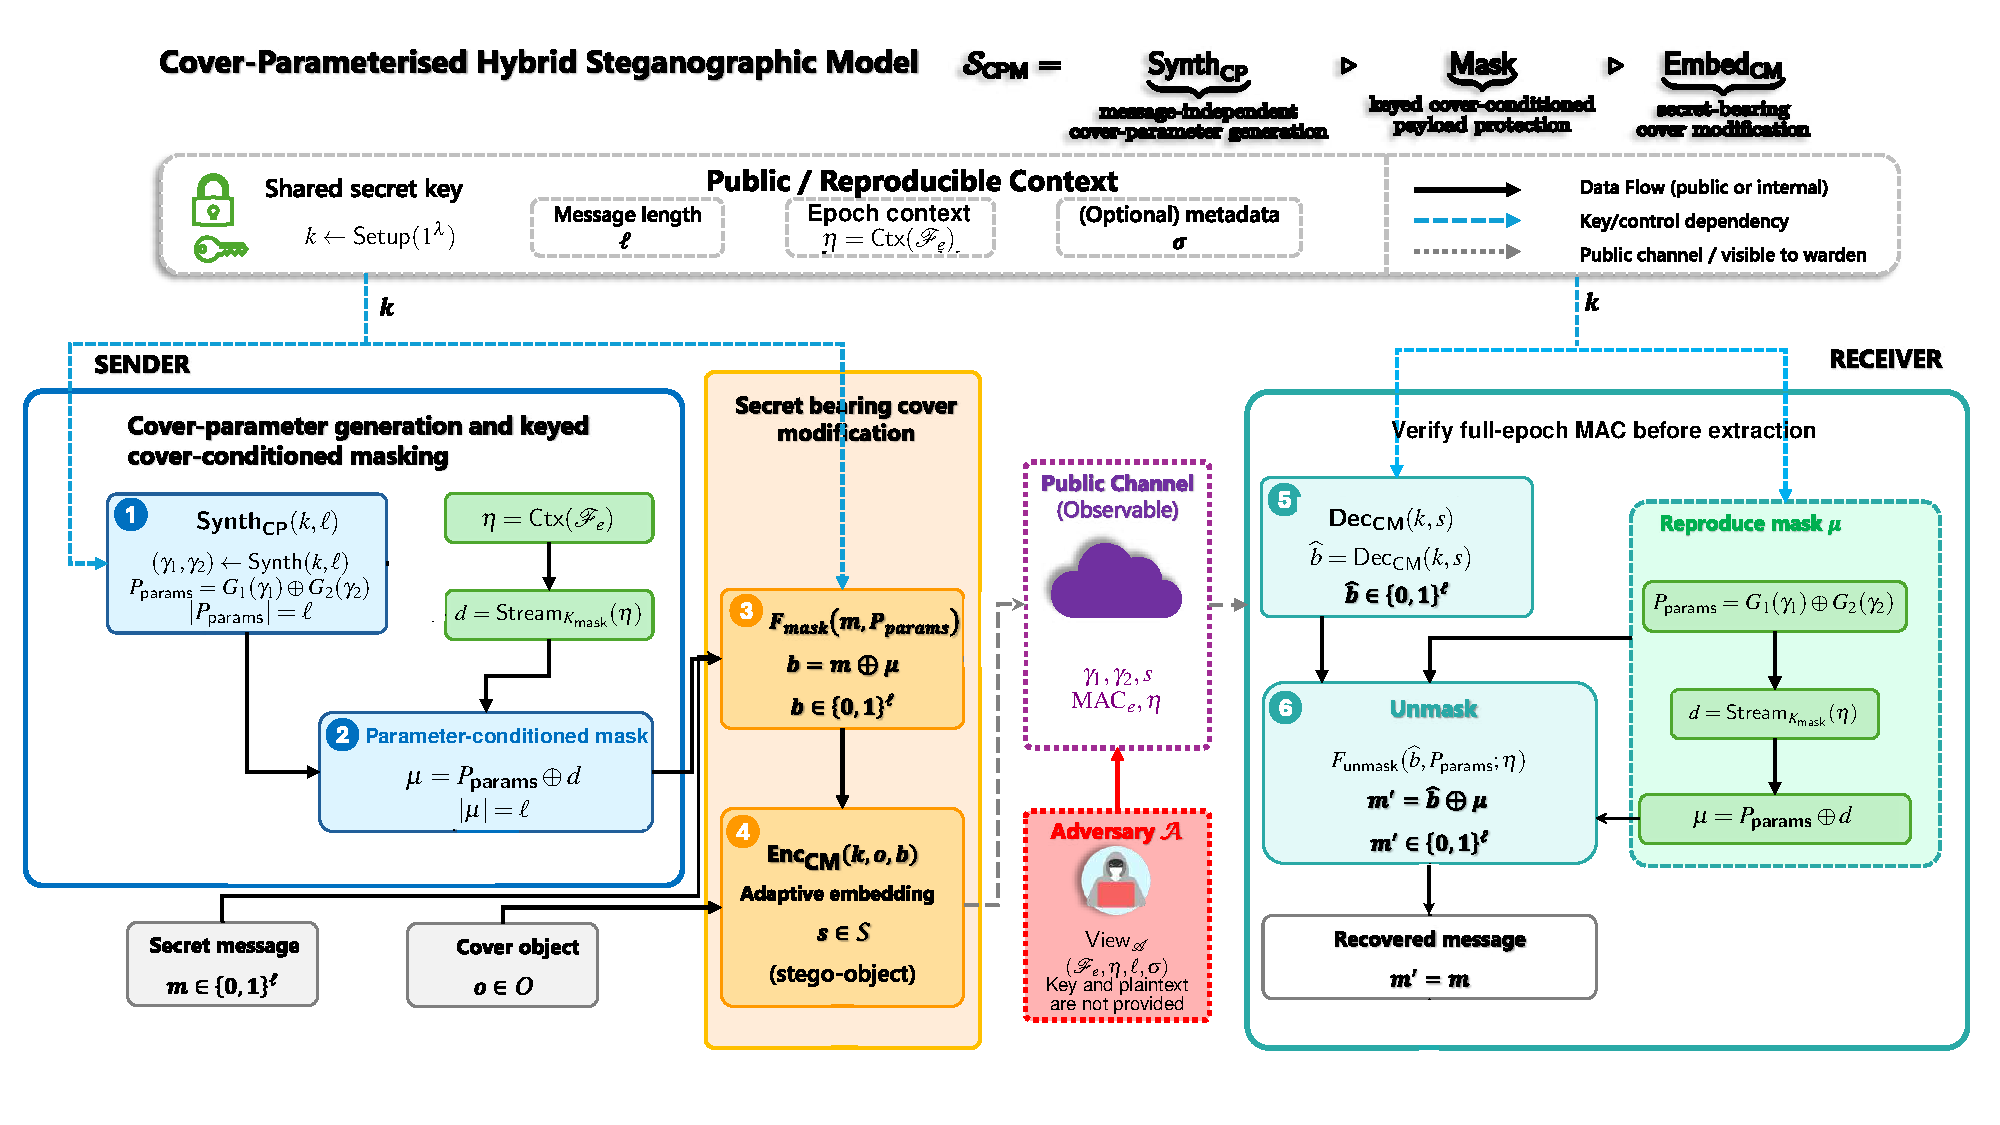
\includegraphics[width=\linewidth]{Figure_1.pdf}
\caption{The Cover-Parameterised Multichannel Hybrid Steganographic Model.
The six-stage architecture combines synthesis, masking and embedding. Public parameters determine
$P_{\mathsf{params}}$, and $d\equiv\rho_{\mathsf{dit}}$ denotes the separate
keyed stream. $\mathsf{Ctx}$ selects only the public epoch fields of
Eq.~\eqref{eq:receiver-context}, generated before embedding. The receiver
verifies the complete epoch before extraction and reconstructs the same mask
from received fields. The equality $m'=m$ is conditional on successful decoding.}
\label{fig:hybrid-entropy-stego-model}
\end{figure*} 

\section{The Proposed Steganographic System Model}
\label{Hybrid_stego_model}
This section introduces a \emph{Cover-Parameterised Multichannel Hybrid Steganographic Model}, denoted by
$\mathcal{S}_{\mathsf{CPM}}$. The model does not use conventional CSY to generate a secret-bearing cover; instead, it employs message-independent synthesis to produce cover-parameter objects suggestive of natural content that condition a keyed masking process through a cover-conditioned dither. The resulting masked payload is then embedded into an existing cover using CMO. This synthesis--modification architecture is referred to as \emph{Steganography by Cover-Parameterised Modification (CPM)}. Algorithm~\ref{alg:HybridStegoModel} outlines the operational flow of $\mathcal{S}_{\mathsf{CPM}}$.

\subsection{Overview and Rationale}

The motivation for CPM arises from the complementary properties of synthesis and cover modification. Conventional CMO provides a practical mechanism for embedding payloads into existing covers, but the resulting modifications may introduce detectable statistical artefacts. Conventional CSY avoids modifying an existing cover by generating the secret-bearing object directly, but may incur substantial generation cost, domain dependence, or
capacity constraints. CPM adopts a different hybrid architecture: message-independent synthesis produces innocuous cover-parameter objects, while the actual concealed payload is carried by an adaptively modified cover. Thus, the synthesis component provides
auxiliary conditioning information rather than a secret-bearing cover.

The resulting separation creates distinct security roles for the cover-parameter, masking, embedding, and multichannel transport layers (see Section~\ref{Hybrid_Entropy_Steganographic_Communication_Protocol} for details). Cover parameters must remain benign and difficult to link to the stego-object; the keyed cover-conditioned mask protects the payload; the embedding stage controls the modification footprint; and the multichannel scheduler limits correlations introduced by
transport. These leakage sources are formalised separately and combined in the security analysis of
Theorem~\ref{thm:composition}. Figure~\ref{fig:hybrid-entropy-stego-model} illustrates the resulting separation between cover-parameter synthesis, cover-conditioned masking, and final cover modification.

Section~\ref{Hybrid_Entropy_Steganographic_Communication_Protocol} will later illustrate how these steps fit into a communication protocol and how they seamlessly interact with integrity checks and multichannel architectures.

\paragraph{Functions and justification of the combined methods.}
The components solve different problems and are not interchangeable.
\begin{enumerate}[label=(\roman*),leftmargin=2.1em,itemsep=0.3em]
\item \emph{Public parameter synthesis and secret masking.}
Message-independent synthesis supplies the public objects on $C_1$ and
$C_2$ without directly encoding the message in their selection. Their
public bit maps condition the mask, while the independently keyed pseudorandom-function (PRF)
stream protects message content. Public synthesis adds no secret entropy;
a direct PRF mask could provide confidentiality without it. The separate
sampler and linkage premises are needed to justify transmitting these
auxiliary objects inconspicuously. In CPM, a cover parameter is public
contextual input to the reproducible mask; it is not a message-selected
cover or a generated carrier that itself encodes the payload. Message
independence removes a direct payload-selection constraint from the
auxiliary sampler and permits its distribution to be assessed separately
from the message-to-carrier encoder. It is an architectural choice, not a
necessity for PRF-based confidentiality. CP-IND asks whether the observable
parameters resemble the declared benign source; CP-UNL asks whether their
content reveals additional coupling to the carrier, conditional on matched
public metadata. Matching visible headers still associate frames. Neither
notion treats public parameters as secret key material.
\item \emph{Adaptive distortion costs.}
QIM-Fused-CF uses quantisation index modulation (QIM)-inspired
cost modulation. The fused cost map combines S-UNIWARD-style residual sensitivity with a
MiPOD-inspired statistical-detectability criterion
\cite{holub2014universal,sedighi2015content}. Complex-feature refinement favours
textured locations, Simple Linear Iterative Clustering (SLIC) supplies
coherent regions, and local cost
spreading discourages isolated changes \cite{setiadi2025maximizing,achanta2012slic,li2014new}.
The QIM-inspired dither modulates these sender-side costs; it is distinct
from the receiver's PRF/XOR payload mask. These are design choices, not
separately proved sources of undetectability; attributing a benefit to
individual terms requires controlled ablations.
\item \emph{Syndrome-trellis coding.}
STC translates the selected costs into coded pixel changes with low
additive distortion \cite{Filler2011STC}. It supplies the embedding/extraction
mechanism, not encryption or authentication. Extraction uses the received
image and agreed coding seed, so the receiver does not need the sender's
cost map.
\item \emph{Epoch authentication and freshness.}
Domain-separated HMAC authenticates the complete three-channel transcript
\cite{bellare1996keying,rfc2104}. This prevents a parameter substitution
from silently changing unmasking. Persistent accepted-epoch and nonce
state additionally rejects old authentic traffic; a valid MAC alone cannot
distinguish an old epoch from its replay.
\item \emph{Scheduling and alignment.}
Bounded scheduling controls the intended timing/metadata process, while
windows, timeouts and heartbeats align delayed or reordered frames.
Alignment supports delivery; trace indistinguishability needs a separate
benign-traffic comparison. Neither mechanism guarantees delivery against
an adversary that suppresses all usable epochs.
\end{enumerate}
The contribution is the specified composition and its separate failure
budgets, rather than the invention of S-UNIWARD, MiPOD, SLIC, STC or HMAC.

\paragraph{Concrete composition scenarios.}
An observer can distinguish a joint trace from benign multi-object traffic
through repeated size patterns or unusually synchronised transmissions,
even when each object's marginal appearance is innocuous. Separately, an
intermediary can substitute a public parameter and alter unmasking if a
tag authenticates only the image, or splice authentic components if the
reconstruction fields are not bound to one epoch. Finally, an intact
previously accepted epoch can pass a stateless authentication check when
persistent freshness state is absent. These are conditional failure modes
of incomplete compositions, not claimed attacks against the cited
constructions. CPM assigns them to joint scheduling/metadata analysis,
complete-transcript authentication and receiver-state requirements;
CP-UNL separately concerns additional content coupling beyond the public
frame association. The canonical transcript and acceptance predicate in
Section~\ref{sec:adversary-operational} make those boundaries explicit.

\subsection{Formal Definition of the Cover-Parameterised Model}\label{hybrid_model}
\begin{definition}[Cover-Parameterised Model]\label{definition_Hybrid_stego}
\emph{A Cover-Parameterised Multichannel Hybrid Steganographic Model is a
hybrid architecture coupling message-independent parameter synthesis,
keyed masking, and cover-modification embedding. Its algorithmic tuple is}
\[
\mathcal S_{\mathsf{CPM}}=
\bigl(\mathsf{Setup},\mathsf{Synth}_{\mathsf{CP}},F_{\mathsf{mask}},
\mathsf{Enc}_{\mathsf{CM}},\mathsf{Dec}_{\mathsf{CM}},F_{\mathsf{unmask}}\bigr),
\]
\emph{with the architectural composition}
\[
\mathcal S_{\mathsf{CPM}}=
\underbrace{\mathsf{Synth}_{\mathsf{CP}}}_{\substack{\text{message-independent}\\\text{cover-parameter generation}}}
\triangleright
\underbrace{\mathsf{Mask}}_{\substack{\text{keyed parameter-conditioned}\\\text{payload protection}}}
\triangleright
\underbrace{\mathsf{Embed}_{\mathsf{CM}}}_{\substack{\text{secret-bearing}\\\text{cover modification}}}.
\]
Here $\triangleright$ denotes sequential composition. The following six
algorithms are efficient in the security parameter $\lambda$ and input
lengths. In these signatures, $k$ denotes the provisioned
secret-key record, and the public epoch context $\eta_e$ is fixed for each
invocation. Where needed, we write $\mathsf{Enc}_{\mathsf{CM}}(k,o,b;\eta_e)$
and $\mathsf{Dec}_{\mathsf{CM}}(k,s;\eta_e)$ to make that context explicit;
it is not additional secret key material. We use the shorthand
$\mathsf{Enc}\equiv\mathsf{Enc}_{\mathsf{CM}}$ and
$\mathsf{Dec}\equiv\mathsf{Dec}_{\mathsf{CM}}$.
\begin{enumerate}[label=(\Alph*),leftmargin=2em]
\item $\boldsymbol{\mathsf{Setup}}(\lambda)$.
Write $\mathsf{Setup}(\lambda)\equiv\mathsf{Setup}(1^\lambda)$.
Setup provisions a secret master key $k=V_{\mathsf{pri}}$ and the agreed
algorithm suite. Session-specific purpose keys are derived by the labelled
HMAC construction in Section~\ref{sec:ProtocolSetup}:
\[
\begin{gathered}
K_L=\mathsf{KDF}_{k}(v,\mathsf{sid},L),\qquad\\
L\in\{\mathsf{header},\mathsf{nonce},\mathsf{mask},\mathsf{emb},
\mathsf{cost},\mathsf{mac}\}.
\end{gathered}
\]
The purpose names above abbreviate the exact byte labels in Section~\ref{sec:ProtocolSetup}. A keyed sampler, when used, has its own separated key. Original covers
are sampled independently of message values conditional on the permitted
public length/format class. Session identifiers
and epoch numbers must not be reused. The image validation worker accepts
pre-generated parameter fixtures; it does not re-evaluate the sampler.

\item $\boldsymbol{\mathsf{Synth}_{\mathsf{CP}}}(k,\ell)$.
The sampler obtains two publicly observable objects independently of message
values, conditional on permitted public length/format metadata:
\[
(\gamma_{1,e},\gamma_{2,e})\leftarrow\mathsf{Synth}(k,\ell_e),
\qquad \ell_e=|m_e|.
\]
Its parameter realisation is
\begin{equation}\label{eq:Pparams}
\begin{aligned}
P_{\mathsf{params},e}
 &=\mathsf{ParamExtract}_{\ell_e}(\gamma_{1,e},\gamma_{2,e})\\
 &=G_{1,\ell_e}(\gamma_{1,e})\oplus G_{2,\ell_e}(\gamma_{2,e})
 \in\{0,1\}^{\ell_e}.
\end{aligned}
\end{equation}
The original PRNG notation denotes the sampler's coin expansion:
\[
R_e\leftarrow F_{\mathsf{PRNG}}(K_{\mathsf{synth}},\mathsf{ctx}_e;r),\qquad
(\gamma_{1,e},\gamma_{2,e})=\mathsf{Samp}(R_e;\ell_e).
\]
Here $r$ is the domain adapter's coin budget, not necessarily the message
length. This PRNG stage does not make its publicly transmitted outputs secret.
Thus $\mathsf{Synth}_{\mathsf{CP}}$ denotes sampling plus public parameter
extraction; $\mathsf{Synth}$ denotes the object-sampling component.
The reference $G_{j,\ell}$ maps exact object bytes through domain-separated
SHAKE256 and truncates to $\ell$ bits. Its output is public and supplies no
additional secret entropy. Message independence does not imply benign
sampling: the separate sampler loss is defined in Section~\ref{subsec:main-theorem}.

\item $\boldsymbol{F_{\mathsf{mask}}}(m,P_{\mathsf{params}};\eta)$.
Generate all three channel nonces before masking and define
\begin{equation}\label{eq:receiver-context}
\eta_e=\mathsf{Encode}(v,\mathsf{sid},H_e,n_{a,e},n_{b,e},n_{c,e},
 \ell_e,\mathsf{codec}),\qquad H_e=(e,N_e).
\end{equation}
Every field is received or pre-agreed and authenticated. Define the
PRF-expanded dither stream and binary mask by
\[
d_e\equiv\rho_{\mathsf{dit},e}
=\mathsf{Stream}_{K_{\mathsf{mask}}}(\texttt{payload-mask},\eta_e,\ell_e),
\qquad \mu_e=P_{\mathsf{params},e}\oplus d_e.
\]
Then
\begin{equation}\label{eq:qim_mask}
b_e=F_{\mathsf{mask}}(m_e,P_{\mathsf{params},e};\eta_e)
=m_e\oplus\mu_e.
\end{equation}
This is one parameter-conditioned PRF/XOR construction. Mask reconstruction uses received fields and does not require original-image
features. The label $d$ in Figure~\ref{fig:hybrid-entropy-stego-model}
denotes this same stream, not a second masking rule.

\item $\boldsymbol{\mathsf{Enc}_{\mathsf{CM}}}(k,\,o,\,b)$.
The adaptive encoder maps $o_e\in\mathcal O$ and $b_e\in\{0,1\}^{\ell_e}$
to $s_e\in\mathcal S$. In the image instantiation, original-image features
are used only at the sender for separately keyed cost modulation:
\[
u_i=\mathsf{CostDither}(K_{\mathsf{cost}},\eta_e,\Psi(o_e),i),\qquad
\rho_i^\pm=\mathsf{Cost}^{\pm}(o_e,\Psi(o_e),u_i).
\]
With $z_e=\mathsf{Seed}(K_{\mathsf{emb}},\eta_e)$,
\[
s_e=\mathsf{Enc}_{\mathsf{CM}}(k,o_e,b_e)
=\mathsf{STC.Enc}(o_e,b_e;\rho_e^-,\rho_e^+,z_e).
\]
The feature digest $\zeta_e=\Phi(o_e)=\mathsf{FeatureDigest}(\Psi(o_e))$
is used only by sender cost modulation; it is not a receiver masking input. QIM-inspired modulation belongs to these adaptive costs; STC performs the
pixel embedding. The sender verifies extraction before emitting an epoch.
Padding and backend length-header bits are separate from $\ell_e$.

\item $\boldsymbol{\mathsf{Dec}_{\mathsf{CM}}}(k,\,s)$.
After verifying the complete received epoch, the receiver reconstructs
$\eta_e$ from its frames and computes
\[
\widehat b_e=\mathsf{Dec}_{\mathsf{CM}}(k,s_e)
=\mathsf{STC.Dec}(s_e;\mathsf{Seed}(K_{\mathsf{emb}},\eta_e)).
\]
The decoder checks the native byte count $\lceil\ell_e/8\rceil$, removes the fixed byte padding, and returns the logical $\ell_e$-bit intermediary. It returns $\bot$ on failure or incompatible decoded length.
Neither $o_e$, $\Psi(o_e)$, nor the sender's cost map is a receiver input.

\item $\boldsymbol{F_{\mathsf{unmask}}}(b,P_{\mathsf{params}};\eta)$.
The receiver applies the same public maps and keyed stream to authenticated
received bytes, giving
\begin{equation}\label{eq:qim_unmask}
\begin{aligned}
\widehat m_e
 &=F_{\mathsf{unmask}}(\widehat b_e,P_{\mathsf{params},e};\eta_e)\\
 &=\widehat b_e\oplus P_{\mathsf{params},e}\oplus
 \mathsf{Stream}_{K_{\mathsf{mask}}}(\texttt{payload-mask},\eta_e,\ell_e).
\end{aligned}
\end{equation}
\end{enumerate}
For each valid key and admissible payload $1\le|m|\le\mathsf{Pol}(|o|)$, the
required algebraic correctness identity is
\[
\begin{aligned}
m=F_{\mathsf{unmask}}\!\Bigl(
 &\mathsf{Dec}_{\mathsf{CM}}\!\bigl(k,
 \mathsf{Enc}_{\mathsf{CM}}(k,o,F_{\mathsf{mask}}(m,P_{\mathsf{params}};\eta))\bigr),\\
 &P_{\mathsf{params}};\eta\Bigr).
\end{aligned}
\]
whenever $\mathsf{Dec}_{\mathsf{CM}}$ correctly inverts the selected embedding.
Capacity admissibility alone does not guarantee error-free STC inversion.
\end{definition}

\begin{algorithm}[H]
\footnotesize
\caption{$\mathcal S_{\mathsf{CPM}}$ with Parameter-Conditioned Masking}
\label{alg:HybridStegoModel}
\KwIn{$\lambda,m,o$; shared $k$; fresh $(\mathsf{sid},e)$ and agreed codec}
\KwOut{Frames $\mathcal F_{1,e},\mathcal F_{2,e},\mathcal F_{3,e}$; recovered $m'$ or $\bot$}
\textbf{1. Setup and parameter generation}\;
$k\leftarrow\mathsf{Setup}(\lambda)$ if not already provisioned; $\ell\leftarrow|m|$\;
$(\gamma_1,\gamma_2)\leftarrow\mathsf{Synth}(k,\ell)$;
$P_{\mathsf{params}}\leftarrow G_{1,\ell}(\gamma_1)\oplus G_{2,\ell}(\gamma_2)$\;
$(H_e,n_a,n_b,n_c)\leftarrow\mathsf{EpochFields}(k,\mathsf{sid},e)$\;
$\eta\leftarrow\mathsf{Encode}(v,\mathsf{sid},H_e,n_a,n_b,n_c,\ell,\mathsf{codec})$\;
\BlankLine
\textbf{2. Parameter-conditioned masking}\;
$d\leftarrow\mathsf{Stream}_{K_{\mathsf{mask}}}(\texttt{payload-mask},\eta,\ell)$;
$\mu\leftarrow P_{\mathsf{params}}\oplus d$\;
\For{$i\leftarrow1$ \KwTo $\ell$}{$b[i]\leftarrow m[i]\oplus\mu[i]$\;}
\BlankLine
\textbf{3. Adaptive encoding}\;
$\Psi\leftarrow\mathsf{Features}(o)$; $u\leftarrow\mathsf{CostDither}(K_{\mathsf{cost}},\eta,\Psi)$\;
$\rho^\pm\leftarrow\mathsf{QIM\text{-}Fused\text{-}CF}(o,\Psi,u)$;
$z\leftarrow\mathsf{Seed}(K_{\mathsf{emb}},\eta)$\;
$s\leftarrow\mathsf{STC.Enc}(o,b;\rho^-,\rho^+,z)$\;
\If{$\mathsf{STC.Dec}(s;z)\ne b$}{\Return $\bot$ \tcp*[r]{sender preflight}}
\BlankLine
\textbf{4. Complete-epoch authentication and transmission}\;
$\mathcal T_e\leftarrow\mathsf{Encode}_{\mathsf{epoch}}(\eta,(C_1,n_a,\gamma_1),(C_2,n_b,\gamma_2),(C_3,n_c,s))$\;
$t_e\leftarrow\mathsf{HMAC}_{K_{\mathsf{mac}}}(\texttt{epoch}\parallel\mathcal T_e)$\;
Construct $\mathcal F_{j,e}$ by Eq.~\eqref{eq:trans}; send on $C_j$, $j\in\{1,2,3\}$\;
\BlankLine
\textbf{5. Receiver verification and extraction}\;
$\widehat{\mathcal F}_e\leftarrow\mathsf{ParseAlign}(\mathcal F_{1,e},\mathcal F_{2,e},\mathcal F_{3,e})$\;
\If{$\neg\mathsf{VerifyEpoch}(k,\widehat{\mathcal F}_e,\mathsf{State})$}{\Return $\bot$}
$\widehat\eta\leftarrow\mathsf{Ctx}(\widehat{\mathcal F}_e)$;
$\widehat b\leftarrow\mathsf{Dec}_{\mathsf{CM}}(k,\widehat s;\widehat\eta)$\;
\If{$\widehat b=\bot$ or $\mathsf{BitLength}(\widehat b)\ne\ell$}{\Return $\bot$}
\BlankLine
\textbf{6. Receiver-only unmasking}\;
$\widehat P\leftarrow G_{1,\ell}(\widehat\gamma_1)\oplus G_{2,\ell}(\widehat\gamma_2)$;
$\widehat d\leftarrow\mathsf{Stream}_{K_{\mathsf{mask}}}(\texttt{payload-mask},\widehat\eta,\ell)$\;
\For{$i\leftarrow1$ \KwTo $\ell$}{$m'[i]\leftarrow\widehat b[i]\oplus\widehat P[i]\oplus\widehat d[i]$\;}
\BlankLine
\textbf{7. Commit and output}\;
\If{$\neg\mathsf{CommitFreshness}(\mathsf{sid},e,n_a,n_b,n_c)$}{\Return $\bot$}
\Return $m'$ \tcp*[r]{no original cover or sender plaintext is consulted}
\end{algorithm}

\begin{theorem}[Conditional correctness of $\mathcal S_{\mathsf{CPM}}$]
\label{thm:CorrectnessHybrid}
Let $k\leftarrow\mathsf{Setup}(1^\lambda)$, $1\le\ell=|m|\le\mathsf{Pol}(|o|)$,
and let $s=\mathsf{Enc}_{\mathsf{CM}}(k,o,b)$ be received in an unaltered,
valid authenticated epoch. Canonical reconstruction gives
\[
\widehat\eta=\eta,\qquad
\widehat P_{\mathsf{params}}=P_{\mathsf{params}},\qquad
\widehat\mu=\mu.
\]
Consequently,
\[
\mathsf{Dec}_{\mathsf{CM}}(k,s)=b
\quad\Longrightarrow\quad
F_{\mathsf{unmask}}(\mathsf{Dec}_{\mathsf{CM}}(k,s),P_{\mathsf{params}};\eta)=m.
\]
If $\Pr[\mathsf{Dec}_{\mathsf{CM}}(k,s)\ne b]\le\delta_{\mathsf{dec}}$ for
these valid epochs, then
\[
\Pr[\mathsf{Accept}_e\wedge\widehat m_e\ne m_e]\le\delta_{\mathsf{dec}}.
\]
\end{theorem}
\begin{proof}
The public maps act on identical received bytes, and the keyed stream uses
the same authenticated context. Thus
\[
\widehat m=(m\oplus\mu)\oplus\widehat\mu
=m\oplus(\mu\oplus\mu)=m
\]
whenever decoding returns $b$. Any accepted plaintext error must therefore
lie in the decoder-failure event, proving the probability bound. No
invariance of $\Psi(o)$ under embedding is assumed.
\end{proof}

The tuple above specifies the model's algorithmic interfaces and conditional
correctness. Section~\ref{Hybrid_Entropy_Steganographic_Communication_Protocol}
instantiates them as authenticated multichannel epochs, and
Section~\ref{sec:security} analyses the corresponding security goals and losses.


\begingroup
\scriptsize
\renewcommand{\arraystretch}{1.0}
\begin{longtable}{|c|p{5.0cm}|}
\caption{Description of Notation}\label{tab:notation_description}\\
\hline
\textbf{Symbol} & \textbf{Definition} \\ \hline
\endfirsthead
\caption[]{Description of Notation (continued)}\\
\hline
\textbf{Symbol} & \textbf{Definition} \\ \hline
\endhead
$m \in \mathcal{M}$ & Secret message; $\ell = |m|$ is its bit length. \\ \hline
$\ell = |m|$ & Length of secret message $m$. \\ \hline
$k \in \mathcal{K}$ & Provisioned master key $k=V_{\mathsf{pri}}$ from $\mathsf{Setup}(1^\lambda)$. \\ \hline
$V_{\mathsf{pri}}$ & Master secret used to derive the separated purpose keys. \\ \hline
$P_{\mathsf{params}} \in \{0,1\}^{\ell}$ & Public parameter bitstream from Eq.~\eqref{eq:Pparams}. \\ \hline
$b_e$ & Masked payload $b_e=m_e\oplus\mu_e$; see Eq.~\eqref{eq:qim_mask}. \\ \hline
$o \in \mathcal{O}$ & Cover object; $s \in \mathcal{S}$ is the resulting stego object. \\ \hline
$\gamma_1,\gamma_2 \in \mathcal{O}'$ & Synthesized cover messages sent on $C_1,C_2$. \\ \hline
$K_{\mathsf{mask}},K_{\mathsf{emb}},K_{\mathsf{mac}}$ & Distinct purpose keys derived from the master secret and session. \\ \hline
$k_{\mathsf{stego},e}=\mathsf{Seed}(K_{\mathsf{emb}},\eta_e)$ & STC permutation seed; a coding parameter, not the confidentiality key. \\ \hline
$\mathrm{HMAC},\,\mathsf{H}$ & Keyed PRF/MAC and public hash; key separation is an explicit computational premise. \\ \hline
$C_1,C_2,C_3$; $\mathcal{C}$ & Channels; $\mathcal{C}=\{1,\dots,c\}$ and $c=|\mathcal{C}|$. \\ \hline
$H_e=(e,N_e)$ & Epoch header authenticated under a separate header key. \\ \hline
$\mathsf{Sched}(\cdot;\sigma)$ & Admissible scheduler with state $\sigma\in\Sigma$. \\ \hline
$W,\tau,\Delta_{\mathsf{time}},h$ & Window size, per-epoch timeout, allowable arrival skew bound, heartbeat period. \\ \hline
$(n,k_{\text{ecc}},t)$ & ECC parameters (length, dimension, $t$ correctable errors/erasures). \\ \hline
$\mathcal{D}_i$ & Cover distribution on channel $i$; draws $o_i\sim\mathcal{D}_i$. \\ \hline
$\mathrm{TV}(\cdot,\cdot)$ & Total variation distance; used in indistinguishability bounds. \\ \hline
$\varepsilon_{\mathsf{param}},\varepsilon_{\mathsf{emb}},\varepsilon_{\mathsf{sched}}(\sigma)$ & Computational masking loss; carrier replacement loss; joint scheduling/metadata loss. \\ \hline
$U_\ell$ & Uniform distribution on $\{0,1\}^{\ell}$. \\ \hline
$\theta$ & Optional domain-adapter synthesis parameter (e.g., variance/latent matching). \\ \hline
$\mathcal{A}$ & PPT adversary/warden (IND-STEGO-MC game). \\ \hline
$F_{\mathsf{PRNG}}:\mathcal K\times\{0,1\}^*\times\mathbb N\to\{0,1\}^*$ & Sampler coin expansion; requested $r$-bit output. \\ \hline
\footnotesize{$F_{\text{mask}}: \mathcal{M} \times \{0,1\}^{\ell} \rightarrow \{0,1\}^\ell$} & Masking function combining $m$ and $P_{\mathsf{params}}$. \\ \hline
$\mathsf{Enc}: \mathcal{O}\times\{0,1\}^{\ell}\rightarrow\mathcal{S}$ & Embedding of masked payload $b$ into cover $o$, with key and authenticated context fixed as in the algorithm interface. \\ \hline
$\mathsf{Dec}: \mathcal{S} \rightarrow \{0,1\}^\ell$ & Extraction function retrieving $b$ from $s$. \\ \hline
{\scriptsize $F_{\text{unmask}}:\{0,1\}^\ell \times \{0,1\}^\ell \rightarrow \mathcal{M}$} & Unmasking function to recover $m$. \\ \hline
$\eta_e,d_e,\mu_e$ & Authenticated public context, keyed stream, and full payload mask. \\ \hline
$\varepsilon_{\mathsf{KDF}},\varepsilon_{\mathsf{samp}}$ & Key-separation loss and independent sampler mismatch. \\ \hline
$\varepsilon_{\mathsf{cp\text{-}ind}},\varepsilon_{\mathsf{cp\text{-}unl}},\varepsilon_{\mathsf{cp}}$ & Parameter opacity, conditional linkage, and their aggregate budget. \\ \hline
$\varepsilon_{\mathsf{unl}}$ & Conditional content/tag-privacy transition loss. \\ \hline
$\mathcal E_{\mathsf{acc}},\mathcal N_{\mathsf{acc}}$ & Protected accepted-epoch and nonce state. \\ \hline
$\delta_{\mathsf{dec}},\delta_{\mathsf{fresh}},\delta_{\mathsf{state}}$ & Decoder, uniqueness, and protected-state failure budgets. \\ \hline
\end{longtable}
\endgroup

\section{Hybrid Steganographic Communication Protocol}
\label{Hybrid_Entropy_Steganographic_Communication_Protocol}
The protocol $\mathcal P^{\mathsf{cs,cm}}_{\mathsf{hyb\text{-}stego}}$
uses the single masking construction in Eqs.~\eqref{eq:Pparams}--\eqref{eq:qim_unmask}.
The executable instantiation is identified as \texttt{cpm-epoch-v2}.

\subsection{Protocol Description}\label{proto_Des}
\subsubsection{Setup and shared parameters}\label{sec:ProtocolSetup}
The endpoints share $V_{\mathsf{pri}}$ and agree on a fresh 128-bit
session identifier, protocol version, and codec. For each purpose $L$, derive
\[
K_L=\mathsf{HMAC}_{V_{\mathsf{pri}}}
 \bigl(\texttt{derive}\parallel\mathsf{Encode}(v,\mathsf{sid},L)\bigr).
\]
Distinct labels identify header, nonce, payload-mask, embedding, cost-modulation,
and epoch-MAC keys. Secure provisioning and persistent session/epoch state are
endpoint requirements. Purpose keys depend on the session and purpose labels, not on the public
parameter objects.
We abbreviate the header-purpose key $K_{\mathsf{header}}$
as $K_{\mathsf{hdr}}$ below.
For epoch $e$ define
\[
N_e=\mathsf{HMAC}_{K_{\mathsf{hdr}}}(\texttt{hdr}\parallel\mathsf{uint64}(e))_{[128]},
\qquad H_e=(e,N_e).
\]
The three 128-bit nonces use channel-separated PRF inputs under $K_{\mathsf{nonce}}$.
An epoch identifier is not reused within a session. The receiver checks
distinctness and freshness; collisions cause rejection. Window $W$, timeout
$\tau$, and permitted inter-channel skew $\Delta_{\mathsf{time}}$ control alignment.
Concrete ECC is not implemented in the reference protocol.

\subsubsection{Phases of the protocol}\label{ProtocolPhases}
Amara obtains two message-independent parameter objects, generates all header
and nonce fields, and constructs $\eta_e$. She masks $m_e$ and embeds $b_e$
using sender-side adaptive costs. Ebere reconstructs the same mask from the
received authenticated fields; she never needs the original image or its cost map.

\begin{algorithm}[H]
\footnotesize
\caption{Message Encoding and Complete-Epoch Authentication}
\label{alg:MessageEncoding}
\KwIn{$V_{\mathsf{pri}},\mathsf{sid},e,m_e,o_e,\gamma_{1,e},\gamma_{2,e}$}
\KwOut{$\mathcal F_{1,e},\mathcal F_{2,e},\mathcal F_{3,e}$ or $\bot$}
\textbf{E1 (Purpose keys).}
\ForEach{agreed purpose label $L$}{
$K_L\leftarrow\mathsf{HMAC}_{V_{\mathsf{pri}}}
(\texttt{derive}\parallel\mathsf{Encode}(v,\mathsf{sid},L))$\;
}
\textbf{E2 (Fresh public context).}
$\ell_e\leftarrow|m_e|$;
$N_e\leftarrow\mathsf{HMAC}_{K_{\mathsf{hdr}}}(\texttt{hdr}\parallel\mathsf{uint64}(e))_{[128]}$;
$H_e\leftarrow(e,N_e)$\;
\ForEach{$j\in\{1,2,3\}$}{
$n_{j,e}\leftarrow\mathsf{HMAC}_{K_{\mathsf{nonce}}}(\texttt{C}j\parallel\mathsf{uint64}(e))_{[128]}$\;
}
$\eta_e\leftarrow\mathsf{Encode}(v,\mathsf{sid},H_e,n_{1,e},n_{2,e},n_{3,e},\ell_e,\mathsf{codec})$\;
\textbf{E3 (Public extraction and one mask).}
$P_e\leftarrow G_{1,\ell_e}(\gamma_{1,e})\oplus G_{2,\ell_e}(\gamma_{2,e})$\;
$d_e\leftarrow\mathsf{Stream}_{K_{\mathsf{mask}}}(\texttt{payload-mask},\eta_e,\ell_e)$;
$\mu_e\leftarrow P_e\oplus d_e$;
$b_e\leftarrow m_e\oplus\mu_e$\;
\textbf{E4 (Adaptive embedding and preflight).}
$s_e\leftarrow\mathsf{Enc}_{\mathsf{CM}}(k,o_e,b_e;\eta_e)$\;
\If{packed native STC extraction does not equal the packed $b_e$}{record failure; \Return $\bot$}
\textbf{E5 (Authenticate every channel).}
$\mathcal T_e\leftarrow\mathsf{Encode}_{\mathsf{epoch}}
(\eta_e,(C_1,n_{1,e},\gamma_{1,e}),(C_2,n_{2,e},\gamma_{2,e}),(C_3,n_{3,e},s_e))$\;
$t_e\leftarrow\mathsf{HMAC}_{K_{\mathsf{mac}}}(\texttt{epoch}\parallel\mathcal T_e)$\;
$\mathcal F_{1,e}\leftarrow(v,\mathsf{sid},H_e,n_{1,e},\gamma_{1,e})$\;
$\mathcal F_{2,e}\leftarrow(v,\mathsf{sid},H_e,n_{2,e},\gamma_{2,e})$\;
$\mathcal F_{3,e}\leftarrow(v,\mathsf{sid},H_e,n_{3,e},\ell_e,\mathsf{codec},s_e,t_e)$\;
\Return $(\mathcal F_{1,e},\mathcal F_{2,e},\mathcal F_{3,e})$\;
\end{algorithm}
The channel indices $(1,2,3)$ correspond to nonce labels $(a,b,c)$ in the
surrounding equations. All nonces precede masking. Sender preflight failures
remain in the attempted-epoch denominator.


\paragraph{One operational mask.}
Equations~\eqref{mask_a_hybrid}--\eqref{eq:qim-dither-mask} expand the
mask $\mu_e$ in Eq.~\eqref{eq:qim_mask}. Step E3 of
Algorithm~\ref{alg:MessageEncoding} implements this same decomposition,
using $P_e\equiv P_{\mathsf{params},e}$ and
$d_e\equiv\rho_{\mathsf{dit},e}$:
\begin{align}\label{mask_a_hybrid}
\mu_e&=G_{1,\ell_e}(\gamma_{1,e})\oplus G_{2,\ell_e}(\gamma_{2,e})
       \oplus\rho_{\mathsf{dit},e},\\
\label{eq:qim-dither-mask}
b_e&=m_e\oplus\mu_e,\qquad
\rho_{\mathsf{dit},e}=\mathsf{Stream}_{K_{\mathsf{mask}}}(\texttt{payload-mask},\eta_e,\ell_e).
\end{align}
The objects are converted to equal-length bitstreams before XOR; raw variable-length
texts are not directly XORed. Original-image features affect only the
sender-side costs through $K_{\mathsf{cost}}$, not the receiver's payload mask.

\paragraph{Authenticated bytes and transmission.}
For compact pseudocode, write $t_e\equiv\mathsf{MAC}_e$.
All variable-length values use the canonical labelled length-prefix encoding.
Define
\begin{equation}\label{eq:epoch-transcript}
\begin{aligned}
\mathcal T_e=\mathsf{Encode}_{\mathsf{epoch}}\bigl(
 &\eta_e,(C_1,n_{a,e},\gamma_{1,e}),\\
 &(C_2,n_{b,e},\gamma_{2,e}),(C_3,n_{c,e},s_e)\bigr).
\end{aligned}
\end{equation}
\begin{equation}\label{MAC}
\mathsf{MAC}_e=\mathsf{HMAC}_{K_{\mathsf{mac}}}
 (\texttt{epoch}\parallel\mathcal T_e).
\end{equation}
The context includes version, session, epoch, header, all nonces, payload length,
and codec. Consequently the tag binds every field controlling reconstruction.
C3 carries the tag, but C1 and C2 are authenticated by the same tag.
The transmitted frames are
\begin{align}\label{eq:trans}
\mathcal F_{1,e}&=(v,\mathsf{sid},H_e,n_{a,e},\gamma_{1,e}),\nonumber\\
\mathcal F_{2,e}&=(v,\mathsf{sid},H_e,n_{b,e},\gamma_{2,e}),\nonumber\\
\mathcal F_{3,e}&=(v,\mathsf{sid},H_e,n_{c,e},\ell_e,\mathsf{codec},s_e,\mathsf{MAC}_e).
\end{align}
In the reference encoding, a field has a two-byte big-endian label length,
label bytes, an eight-byte big-endian value length, and value bytes. Integers
use unsigned eight-byte big-endian encodings. No ambiguous concatenation is used.

\paragraph{Receiver order.}\label{protocol:decodingverification}
After canonical parsing and alignment, Ebere validates the agreed session,
header, payload/codec fields, epoch and nonce freshness, and full-epoch tag:
\begin{equation}\label{MAC Verifi}
\mathsf{MAC}_e\stackrel{?}{=}
 \mathsf{HMAC}_{K_{\mathsf{mac}}}(\texttt{epoch}\parallel\widehat{\mathcal T}_e).
\end{equation}
Only then does she extract $\widehat b_e$ using the key/context-derived STC
seed and unmask by
\begin{equation}\label{unmasked_proto_qim}
\widehat m_e=\widehat b_e\oplus G_{1,\ell_e}(\gamma_{1,e})
 \oplus G_{2,\ell_e}(\gamma_{2,e})\oplus\rho_{\mathsf{dit},e}.
\end{equation}
A missing component, failed check, or incompatible decoded length yields $\bot$.
Freshness state is committed before releasing a recovered message. The sender
reference worker additionally validates STC extraction before emitting an epoch;
all failed attempts must still be counted in correctness reporting.

\begin{lemma}[Protocol correctness]\label{lem:protocol-correctness}
For a valid received epoch, the reconstructed parameters and context are
identical to the sender's. Thus $\widehat b_e=b_e$ implies $\widehat m_e=m_e$.
\end{lemma}
\begin{proof}
Canonical byte reconstruction and the deterministic public mappings give the
same $P_{\mathsf{params},e}$ and $\eta_e$; the keyed stream is therefore equal.
XOR cancellation completes the argument. Decoder errors remain separately
bounded by $\delta_{\mathsf{dec}}$ as in Theorem~\ref{thm:CorrectnessHybrid}.
\end{proof}

\subsection{Multichannel Synchronisation and Re-synchronisation}
\label{subsec:algo-sync}
Section~\ref{proto_Des} specifies \emph{what} is transmitted:
$\mathcal F_{1,e}$ contains $(n_{a,e},\gamma_{1,e})$,
$\mathcal F_{2,e}$ contains $(n_{b,e},\gamma_{2,e})$, and
$\mathcal F_{3,e}$ contains $(n_{c,e},s_e,\mathsf{MAC}_e)$ together with
version, session, header, length and codec fields as in Eq.~\eqref{eq:trans}.
Algorithm~\ref{alg:mc-sync} specifies \emph{how} the sender and receiver
schedule, align, authenticate and reconstruct these objects.

Let $\mathcal W=[a,a+W-1]$ be the receiver's epoch window,
$\mathcal B_j[e]$ its bounded channel buffers, and $t_j[e]$ the arrival
of a selected candidate on $C_j$. For $\sigma\in\Sigma$, readiness requires
\[
\mathsf{Ready}_e\equiv
\bigwedge_{j=1}^{3}(\mathcal B_j[e]\ne\varnothing)
\ \wedge\ (\max_jt_j[e]-\min_jt_j[e]\le\Delta_{\mathsf{time}})
\ \wedge\ (t-t_{\mathsf{first}}[e]\le\tau).
\]
A content-independent $H_e=(e,N_e)$ associates frames publicly; it does not
alone authenticate their contents or imply content unlinkability. The whole
canonical transcript is verified only after the necessary frames are present.

\SetKwBlock{Sender}{Sender (Amara)}{end}
\SetKwBlock{Receiver}{Receiver (Ebere)}{end}
\begin{algorithm}[H]
\footnotesize
\DontPrintSemicolon
\caption{Multichannel Synchronisation and Re-synchronisation (aligned to the protocol)}
\label{alg:mc-sync}
\KwIn{$k,\mathsf{sid}$; messages/covers; $\sigma\in\Sigma$; $W,\tau,\Delta_{\mathsf{time}},h$;
 persistent accepted-epoch/nonce state; expected fragment set $\mathcal E_m$}
\KwOut{Ordered recovered fragments $m'_e$, or $\bot$ for an incomplete message}
\Sender{
\textbf{S1 (Session initialisation).} Derive purpose keys; initialise a non-reused epoch counter $e$\;
\While{message fragments remain}{
\textbf{S2 (Epoch construction).} $e\leftarrow e+1$; $\ell_e\leftarrow|m_e|$;
$(\gamma_{1,e},\gamma_{2,e})\leftarrow\mathsf{Synth}(k,\ell_e)$\;
$N_e\leftarrow\mathsf{HMAC}_{K_{\mathsf{hdr}}}(\texttt{hdr}\parallel\mathsf{uint64}(e))_{[128]}$;
$H_e\leftarrow(e,N_e)$; generate $n_{a,e},n_{b,e},n_{c,e}$\;
Construct $\eta_e,P_{\mathsf{params},e},b_e$ by Eqs.~\eqref{eq:Pparams}--\eqref{eq:qim_mask};
$s_e\leftarrow\mathsf{Enc}_{\mathsf{CM}}(k,o_e,b_e;\eta_e)$\;
\If{sender preflight fails}{record failure; skip this attempted epoch}
Construct $\mathcal T_e$ and full $\mathsf{MAC}_e$ by Eqs.~\eqref{eq:epoch-transcript}--\eqref{MAC}\;
\textbf{S3 ($C_1$).} $\mathsf{Sched}(C_1,\mathcal F_{1,e};\sigma)$\;
\textbf{S4 ($C_2$).} $\mathsf{Sched}(C_2,\mathcal F_{2,e};\sigma)$\;
\textbf{S5 ($C_3$).} $\mathsf{Sched}(C_3,\mathcal F_{3,e};\sigma)$\;
\textbf{S6 (Optional alignment hint).} At cadence $h$, send authenticated header hint
$\mathsf{HB}_e=(v,\mathsf{sid},H_e)$; no hint releases plaintext\;
}
}
\Receiver{
\textbf{R1 (Initialisation).} Restore $\mathcal E_{\mathsf{acc}},\mathcal N_{\mathsf{acc}}$;
set $\mathcal W=[a,a+W-1]$ and $\mathcal B_j[e]\leftarrow\varnothing$\;
\While{frames arrive before application timeout}{
\textbf{R2 (Parse/header checks).} Parse $(\tilde e,\tilde N,j,\mathsf{sid},v)$ canonically\;
\If{wrong session/version/channel, malformed fields, $\tilde e\notin\mathcal W$, or bad $\tilde N$}{discard; continue}
\If{$(\mathsf{sid},\tilde e)\in\mathcal E_{\mathsf{acc}}$ or a received nonce is in $\mathcal N_{\mathsf{acc}}$}{discard; continue}
Buffer the candidate in bounded $\mathcal B_j[\tilde e]$ with timestamp; do not commit freshness\;
\textbf{R3 (Readiness and full integrity).}
\If{$\mathsf{Ready}_{\tilde e}$ and the three channel nonces are distinct}{
Choose a candidate triple; reconstruct $\widehat\eta_{\tilde e},\widehat{\mathcal T}_{\tilde e}$\;
\If{$\widehat{\mathsf{MAC}}_{\tilde e}\ne
\mathsf{HMAC}_{K_{\mathsf{mac}}}(\texttt{epoch}\parallel\widehat{\mathcal T}_{\tilde e})$}{
discard the failed candidate; retain uncommitted state; continue}
\textbf{R4 (Decode and reconstruct).}
$\widehat b_{\tilde e}\leftarrow\mathsf{Dec}_{\mathsf{CM}}(k,\widehat s_{\tilde e};\widehat\eta_{\tilde e})$\;
\If{$\widehat b_{\tilde e}=\bot$ or decoded byte count is incompatible with authenticated $\ell_{\tilde e}$}{discard; continue}
$\widehat P\leftarrow G_{1,\ell}(\widehat\gamma_1)\oplus G_{2,\ell}(\widehat\gamma_2)$;
$\widehat m_{\tilde e}\leftarrow F_{\mathsf{unmask}}(\widehat b_{\tilde e},\widehat P;\widehat\eta_{\tilde e})$\;
Atomically commit $(\mathsf{sid},\tilde e)$ and the three nonces to protected replay state\;
Append the recovered fragment by epoch order; release only after successful state commitment\;
}
\textbf{R5 (Loss/skew and re-synchronisation).}
Expire incomplete candidates after $\tau$; mark unrecovered epochs as erasures\;
Advance the bounded window according to the agreed skip policy;
use a fresh valid $\mathsf{HB}$ only as an alignment hint\;
}
\textbf{R6 (Finalisation).} Reassemble received fragments in epoch order;
output $m'$ if the declared message is complete, otherwise $\bot$\;
}
\end{algorithm}

The sender/receiver transport discipline is specified separately from the
payload algorithms. The \texttt{cpm-epoch-v2} image worker validates already assembled complete
epochs. The timed-receiver adapter evaluated in
Section~\ref{subsec:multichannel_robustness} additionally implements bounded
candidate buffers, skew/timeout checks and a shared-clock window policy,
using saved real-image frames and controlled virtual arrivals. It enables
neither heartbeat recovery nor concrete ECC. Optional coding would require
a specified authenticated codec and actual recovery data; missing C1/C2
parameters are never assumed to be reconstructible. These controlled traces
test receiver operation rather than deployed-network performance.


\subsection{Complexity and Robustness Analysis}\label{subsec:complexity-robustness}
\paragraph{Computational complexity.}
Let $\ell=\sum_{e=1}^{B}\ell_e$ be the application-message length over
$B$ attempted epochs. Write $L_e=|\mathcal T_e|$ for the authenticated
transcript length in bytes, $T_{\mathsf{enc},e}$ for adaptive cost construction
plus embedding, $T_{\mathsf{synth},e}$ for parameter sampling, and
$T_{\mathsf{dec},e}$ for extraction. HMAC costs
$T_{\mathsf{mac}}(L_e)=O(L_e)$; public parameter expansion and mask generation
cost $T_{\mathsf{dither}}(\ell_e)=O(\ell_e)$, with parameter-byte hashing
already covered by $L_e$. The sender/receiver decomposition is
\begin{align*}
T^{(\mathrm{snd})}_e
 &=O\!\Bigl(T_{\mathsf{synth},e}+T_{\mathsf{enc},e}+T_{\mathsf{dec},e}^{\mathsf{pre}}
 +T_{\mathsf{mac}}(L_e)+\ell_e\Bigr),\\
T^{(\mathrm{rev})}_e
 &=O\!\left(T_{\mathsf{dec},e}+T_{\mathsf{mac}}(L_e)
 +\ell_e+T_{\mathsf{state},e}\right).
\end{align*}
Here $T_{\mathsf{dec},e}^{\mathsf{pre}}$ is sender preflight and
$T_{\mathsf{state},e}$ is protected freshness-state commitment. Let $\mathcal V_{\mathsf{dec}}$ index candidate triples that pass
authentication and reach extraction, including any subsequently rejected
for length or state-commit failure. For $q_v$ received candidate triples
and $q_a$ frame arrivals,
\begin{align*}
T^{(\mathrm{snd})}_{\mathrm{total}}
 &=O\!\left(\sum_{e=1}^{B}
 (T_{\mathsf{synth},e}+T_{\mathsf{enc},e}+T_{\mathsf{dec},e}^{\mathsf{pre}}+L_e)+\ell\right),\\
T^{(\mathrm{rev})}_{\mathrm{total}}
 &=O\!\left(\sum_{\nu=1}^{q_v}L_\nu+
 \sum_{\nu\in\mathcal V_{\mathsf{dec}}}
 (T_{\mathsf{dec},\nu}+\ell_\nu+T_{\mathsf{state},\nu})+q_a\right).
\end{align*}
Bookkeeping assumes bounded buffers and expected constant-time indexed
lookups. The reference JSON state file rewrites its accumulated history;
its persistence cost is not assumed constant. Full-image authentication
cannot be costed as a constant-length payload-only MAC.

\paragraph{Communication overhead.}
Let $|H|,|\mathsf{sid}|,|v|,|n_j|,|t|$ denote the binary field lengths.
Separating control information from parameter and carrier bytes gives
\[
\begin{aligned}
O_{\mathsf{ctrl},e}
 &=\underbrace{3(|H|+|\mathsf{sid}|+|v|)}_{\text{common channel fields}}
 +\underbrace{\sum_{j=1}^{3}|n_j|}_{\text{freshness}}\\
 &\quad+\underbrace{|t|}_{\text{complete-epoch integrity}}
 +\underbrace{|\ell_e|+|\mathsf{codec}|+O_{\mathsf{frame},e}}_{\text{decoder/framing fields}},\\
B^{\mathsf{bin}}_e
 &=|\gamma_{1,e}|+|\gamma_{2,e}|+|s_e|+O_{\mathsf{ctrl},e}.
\end{aligned}
\]
For the actual JSON/base64 reference wire, with $x_{1,e}=\gamma_{1,e}$,
$x_{2,e}=\gamma_{2,e}$ and $x_{3,e}=s_e$,
\[
B^{\mathsf{wire}}_e=\sum_{j=1}^{3}
\left(J_{j,e}+4\left\lceil\frac{|x_{j,e}|}{3}\right\rceil\right),
\qquad
B_{\mathsf{total}}=\sum_e B^{\mathsf{wire}}_e+B_{\mathsf{HB}},
\]
where $J_{j,e}$ counts the non-content JSON fields, delimiters and hex
encoding. A specified heartbeat format contributes
$B_{\mathsf{HB}}=O(c\lceil B/h\rceil|\mathsf{HB}|)$.
The binary-layout estimates in Supplementary
Section~\ref{supp-subsec:runtime_overhead} use a different framing model
and do not describe this JSON/base64 wire.
For an optional, separately specified $(n,k_{\mathsf{ecc}},t)$ code,
\[
\ell_{\mathsf{coded}}=n\left\lceil\ell/k_{\mathsf{ecc}}\right\rceil,
\qquad
T_{\mathsf{snd}}\mapsto T_{\mathsf{snd}}+T_{\mathsf{ECC\text{-}enc}},
\quad T_{\mathsf{rev}}\mapsto T_{\mathsf{rev}}+T_{\mathsf{ECC\text{-}dec}}.
\]
The encoded length, codec, framing and actual recovery data would need
complete authentication. Concrete ECC is not enabled in \texttt{cpm-epoch-v2};
these optional interfaces do not imply recovery of absent parameter bytes.

\paragraph{Memory footprint.}
For at most $W$ in-flight epochs, $c$ bounded channel buffers and maximum
retained frame length $L_{\max}$,
\[
\mathsf{Space}=O(WcL_{\max})+
O\!\left(B_{\mathsf{acc}}(|H|+3|n|)\right).
\]
The first term is transient alignment storage; the second is persistent
accepted-epoch/nonce history. The reference worker loads one assembled
epoch rather than implementing the timed window. Session retirement and
rollback protection require an explicit state-lifecycle policy.

\paragraph{Robustness to loss and skew.}
Let $X_j^{(e)}=1$ denote arrival within the agreed timeout/skew policy, and
$p_j=\Pr[X_j^{(e)}=1]$. Then
\[
\pi_{\mathsf{arr}}=\Pr[X_1^{(e)}=X_2^{(e)}=X_3^{(e)}=1],
\qquad
\pi_{\mathsf{use}}=\Pr[\mathsf{Ready}_e\wedge\mathsf{Auth}_e\wedge\mathsf{DecodeOK}_e].
\]
Only under an additional within-epoch channel-independence premise does
$\pi_{\mathsf{arr}}=p_1p_2p_3$. A timely complete triple can still fail
alignment, decoding or state commitment, so it is not automatically a
usable authenticated epoch.

\begin{lemma}[Windowed re-synchronisation bound]\label{lem:resync}
Suppose the transport guarantees at least $n_L$ eligible opportunities
during $L$ epochs following desynchronisation, where $n_L$ is a deterministic
lower bound. If, for every opportunity $j$,
\[
\Pr[E_j\mid E_1^c,\ldots,E_{j-1}^c,\mathsf{network\ state}]
\ge\pi_{\min}>0,
\]
then
\[
\Pr[\text{no re-sync within }L]\le(1-\pi_{\min})^{n_L}.
\]
An eligible success requires complete usable frames, valid full-epoch
verification, decoding and admissible window state. If a further transport
premise guarantees $n_L\ge\lfloor L/h\rfloor$, that lower bound may be
substituted. Heartbeat cadence alone does not establish it or cap delay by $W$.
\end{lemma}
\begin{proof}
By the chain rule,
\[
\Pr\!\left[\bigcap_{j=1}^{n_L}E_j^c\right]
=\prod_{j=1}^{n_L}\Pr[E_j^c\mid E_1^c,\ldots,E_{j-1}^c]
\le(1-\pi_{\min})^{n_L}.
\]
Under independent identically distributed eligible trials of success
probability $\pi$, the expected number of opportunities to success is
$1/\pi$. Converting opportunities to elapsed epochs requires their actual
frequency; frame suppression can prevent all opportunities.
\end{proof}

\paragraph{Correctness under admissible scheduling.}
For an application message with a pre-agreed expected fragment index set
$\mathcal E_m$, let $\delta_{\mathsf{miss}}$ bound missing/unusable fragments
under $\sigma\in\Sigma$. Conditional correctness gives the union bound
\[
\Pr[m'\ne m\ \text{or}\ m'=\bot]
\le\delta_{\mathsf{miss}}+
\sum_{e\in\mathcal E_m}\delta_{\mathsf{dec},e}+\delta_{\mathsf{state}}.
\]
This is an availability/correctness statement for the specified transport
premises. Independently, a security budget
$\varepsilon_{\mathsf{sched}}(\sigma)\le\rho_{\mathsf{dist}}$ bounds a joint
trace-distinguishing transition. A delay bound in milliseconds does not
imply this probability-gap budget.

\paragraph{Integrity, replay, and binding across channels.}
Let $\mathcal E_{\mathsf{acc}}$ and $\mathcal N_{\mathsf{acc}}$ be protected
accepted identifiers and nonces. The acceptance predicate is
\[
\begin{aligned}
\mathsf{Accept}_e={}&\mathsf{Parse}_e\wedge\mathsf{Session}_e\wedge\mathsf{Hdr}_e
\wedge\mathsf{Window}_e\wedge\mathsf{Ready}_e\\
&\wedge\mathsf{Fresh}_e\wedge\mathsf{Tag}_e\wedge\mathsf{Length}_e\wedge\mathsf{Commit}_e,\\
\mathsf{Fresh}_e={}&[(\mathsf{sid},e)\notin\mathcal E_{\mathsf{acc}}]
\wedge\bigwedge_{j\in\{a,b,c\}}[n_{j,e}\notin\mathcal N_{\mathsf{acc}}]\wedge\bigwedge_{i\ne j}[n_{i,e}\ne n_{j,e}],\\
\mathsf{Tag}_e={}&\left[t_e=
\mathsf{HMAC}_{K_{\mathsf{mac}}}(\texttt{epoch}\parallel\mathcal T_e)\right].
\end{aligned}
\]
The canonical $\mathcal T_e$ binds both parameter objects and all
reconstruction fields, as well as the complete image. After key separation,
accepting a new unauthorised $\mathcal T'_e$ supplies a new-message MAC
forgery. In the notation of Section~\ref{sec:integrity},
\[
\Pr[\mathsf{Accept}(\mathcal T'_e)\wedge\mathcal T'_e\notin\mathcal Q_{\mathsf{auth}}]
\le\varepsilon_{\mathsf{KDF}}+\varepsilon_{\mathsf{mac}}
+\delta_{\mathsf{fresh}}+\delta_{\mathsf{state}}.
\]
An exact already accepted replay fails $\mathsf{Fresh}_e$ deterministically
when protected state is intact. Header equality aligns frames; it cannot
replace full-transcript authentication. Rejected header mismatches are
not unauthorised accepts.

\paragraph{Link to indistinguishability.}
The mathematical link has separate, non-overlapping losses:
\[
\begin{aligned}
\mathsf{Adv}^{\mathsf{mc}}_{\mathcal S_{\mathsf{CPM}},\mathbf{\mathcal D}}(\mathcal A;\lambda)
\le{}&\underbrace{\varepsilon_{\mathsf{KDF}}}_{\text{key separation}}+
\underbrace{\varepsilon_{\mathsf{param}}}_{\text{mask pseudorandomness}}+
\underbrace{\varepsilon_{\mathsf{unl}}}_{\text{conditional content linkage}}\\
&+\underbrace{\mathsf{Adv}^{\mathsf{PRF}}_{\mathsf{synth}}+\varepsilon_{\mathsf{samp}}}_{\text{sampler security and independent mismatch}}\\
&+\underbrace{\varepsilon_{\mathsf{emb}}}_{\text{carrier replacement}}+
\underbrace{\varepsilon_{\mathsf{sched}}(\sigma)}_{\text{joint timing/metadata}}.
\end{aligned}
\]
The alternative label $\varepsilon_{\mathsf{dither}}$ denotes the same masking
loss as $\varepsilon_{\mathsf{param}}$; it is not an additional term.
Section~\ref{subsec:main-theorem} defines the games and simulation premises.
Transport acceptance, detector AUC and selected timing statistics do not
numerically upper-bound these aggregate computational losses.

\paragraph{Parameter guidance (practical).}
Under a qualified delay law $F_D$, selecting
$\tau\ge F_D^{-1}(1-\alpha)$ controls the corresponding late-arrival tail
at $\alpha$. Window and heartbeat choices such as
$W\ge\lceil\Delta_{\mathsf{time}}/T_{\mathsf{epoch}}\rceil+1$ and $h\le W$
are alignment design choices requiring separate validation. They do not
guarantee successful delivery or a small $\varepsilon_{\mathsf{sched}}$.
The following assumptions and security games state those premises explicitly.


\subsection{Security Assumptions}
\label{Assumptions}

Each assumption supports a particular guarantee, rather than every claim
requiring the entire list. A1 and the primitive-security parts of A2/A4
are cryptographic premises. The sampler/linkage part of A2, carrier part
of A3 and trace-distribution part of A6 are distributional premises.
Decoding in A3, protected state in A5 and delivery conditions in A6 are
operational requirements. Separating them prevents confidentiality,
concealment, integrity and availability from being treated as one property.

The formal games, Theorem~\ref{thm:composition} and active-attack results use
the following premises; Supplementary Appendix~\ref{supp-subsec:security_assumptions}
gives their detailed formulations. Here $\lambda$ is the security parameter.
The reference profile uses 256-bit purpose keys/tags and 128-bit
nonces/header authenticators. Finite prototype checks do not establish
asymptotic negligible losses.

\begin{enumerate}[
    label=\textbf{A\arabic*.},
    leftmargin=2.3em,
    itemsep=0.35em,
    topsep=0.35em
]

\item \textbf{Key establishment and separation.}
The master secret remains secret and has the stated effective key entropy.
The domain-separated HMAC/KDF purpose-key family is replaceable by independent
keys at computational cost $\varepsilon_{\mathsf{KDF}}$ for the permitted
session/query history. This is the premise of Claim~\ref{Claim1}; a numerical
random-oracle key-query bound for another derivation is not asserted.
This premise justifies independent purpose-key replacements and the
key-secrecy boundary of the network-adversary claim.
Compromised or low-entropy keys invalidate that confidentiality premise.

\item \textbf{Distinct sampler, masking, and linkage premises.}
The real keyed sampler differs from its ideal-coins sampler by the sampler
PRF loss, and the ideal sampler differs from the specified benign joint law
by $\varepsilon_{\mathsf{samp}}$. The mask is pseudorandom jointly with
the public parameters and received context, up to
$\varepsilon_{\mathsf{param}}$. Conditional full-view content linkage is
separately bounded by $\varepsilon_{\mathsf{unl}}$.
These are different premises; neither public parameters nor a good mask
imply a benign sampler. The public epoch context is receiver-reproducible from
authenticated fields, as in Eq.~\eqref{eq:receiver-context}.
A visible sampler bias reveals auxiliary traffic even with a perfect mask;
parameter--carrier dependence can reveal linkage despite benign marginals.
These distributional premises support concealment, whereas the mask PRF
supports message confidentiality. Text and linkage probes test selected
wardens, not the required universal upper bounds.

\item \textbf{Embedding correctness and
indistinguishability.}
For admissible covers, decoding inverts embedding except with
the stated decoding-failure probability. The distribution of the
stego-object on $C_3$ is computationally indistinguishable from
the corresponding cover distribution up to
$\varepsilon_{\mathsf{emb}}$ under the oracle access permitted
by Definition~\ref{def:ind-stego-mc}
\cite{@hopper2009provably,vonahn2003publickey}.
The cover-parameter streams on $C_1$ and $C_2$ are governed by
\textbf{A2} and are not counted again in the embedding term.
Its carrier-distribution premise is used in Theorem~\ref{thm:composition};
its decoding premise is used in Theorem~\ref{thm:CorrectnessHybrid} and
Claim~\ref{Claim4}. Claim~\ref{Claim2} instead uses masking and
message-independent post-processing.
Without decoding correctness an honest authenticated epoch may yield the
wrong message; without the carrier premise a warden may detect its presence
even when the message remains secret. Receiver checks support the former
on tested inputs; detector scores do not prove the latter for all wardens.

\item \textbf{Message-authentication security.}
HMAC is instantiated with a secret, domain-separated key and a
canonical encoding that binds the channel identifier, epoch
header, freshness value, and authenticated content. It is assumed
to be unforgeable under chosen-message attack
\cite{bellare1996keying,rfc2104}. This assumption is used in
Claim~\ref{Claim3}, Claim~\ref{Claim4}, and Theorem~\ref{theoremMTM}. Replay rejection additionally requires the freshness assumption in \textbf{A5}.
Without unforgeability, an attacker may authorise changed parameters or
images. The targeted rejection panel checks the implemented field boundary;
it does not measure a universal MAC-forgery probability.

\item \textbf{Nonce freshness and receiver state.}
The per-channel freshness values are generated from channel-separated PRF inputs and are not intentionally reused under the same
authentication key, and are checked against receiver-maintained
epoch or nonce state \cite{nist80090ar1}. This assumption is used
by Algorithm~\ref{alg:mc-sync}, and Claim~\ref{Claim3}. A verbatim replay is rejected by the
freshness check; random nonce collisions are treated separately
in the detailed supplementary analysis.
A previously valid tag remains valid when replayed, so protected state is
necessary to recognise already accepted traffic. Session/epoch reuse or
state rollback also defeats the intended freshness policy; restart and
concurrent-process behaviour require deployment qualification.

\item \textbf{Admissible scheduling.}
The scheduler belongs to the admissible class $\Sigma$ and
satisfies the delay, skew, burst, timeout, and metadata conditions
required by Algorithm~\ref{alg:mc-sync}. Its residual
cover-versus-protocol timing footprint is bounded by
$\varepsilon_{\mathsf{sched}}(\sigma^\star)$.
The trace premise supports Theorem~\ref{thm:composition}; usable-opportunity
regularity separately supports Lemma~\ref{lem:resync}. Without the first,
content-safe objects may still reveal a distinctive transmission pattern.
Without the second, suppression can prevent re-synchronisation indefinitely.
Delay compliance and synthetic timing tests do not establish benign full traces.

\end{enumerate}

The assumptions exclude endpoint compromise, implementation
side channels, entropy-source failure, and denial-of-service
conditions that prevent protocol delivery altogether.


\section{Security Properties and Discussion}
\label{sec:security}

This section consolidates the guarantees provided by our hybrid protocol $\mathcal{P}^{\mathsf{cs,\,cm}}_{\mathsf{hyb-stego}}$ against multichannel adversaries. We analyse security under the assumptions in Section~\ref{Assumptions}, using the multichannel indistinguishability game and oracles formalised in \S\ref{subsec:formal}, and the hybrid composition bound of Theorem~\ref{thm:composition} in \S\ref{subsec:main-theorem}. Our analysis follows the provable-security tradition in steganography (e.g., the Hopper–Langford–von~Ahn framework and its chosen-hiddentext variants) adapted to multichannel traces and timing/flow shaping \cite{@hopper2009provably,@Hopper2002,vonahn2003publickey}. 

Concretely, the analysis retains three classes of guarantees:
(i) \emph{cover-parameter opacity}, with
$\mathsf{Adv}^{\mathsf{CP\text{-}IND}}\le
\mathsf{Adv}^{\mathsf{PRF}}_{\mathsf{synth}}+\varepsilon_{\mathsf{samp}}$
and conditional content unlinkability bounded by $\varepsilon_{\mathsf{unl}}$;
(ii) \emph{multichannel indistinguishability}, with separate key-derivation,
masking, cover-parameter, carrier and scheduler losses; and
(iii) \emph{active confidentiality/integrity}, with message-recovery advantage
and unauthorised-acceptance probability bounded separately by masking,
complete-epoch MAC, freshness and protected-state premises
\cite{rfc2104,bellare1996keying}. These are conditional reductions; finite
near-chance detection and message independence do not prove all premises.

\subsection{Formal Framework and Security Definition}\label{subsec:formal}
\paragraph{Problem statement.}
A sender $\mathcal U$ transmits $m\in\{0,1\}^{\ell}$ to a receiver
$\mathcal R$ over $c\ge2$ observable channels
$\mathcal C=\{1,\ldots,c\}$. An adaptive PPT warden $\mathcal A$ observes
channel contents and public metadata and may choose admissible timing
policies $\sigma\in\Sigma$. The mapper
$\mathsf{Sched}([c],\mathbf x;\sigma)$ emits timed multichannel traces.
For the three-channel instantiation,
\[
\begin{aligned}
 k&\leftarrow\mathsf{Setup}(1^\lambda),\quad
 (\gamma_{1,e},\gamma_{2,e})\leftarrow\mathsf{Synth}(k,\ell_e),\\
 P_e&=G_{1,\ell_e}(\gamma_{1,e})\oplus G_{2,\ell_e}(\gamma_{2,e}),\quad
 b_e=F_{\mathsf{mask}}(m_e,P_e;\eta_e),\\
 s_e&=\mathsf{Enc}_{\mathsf{CM}}(k,o_e,b_e;\eta_e),\quad
 \mathbf S_e=(\mathcal F_{1,e},\mathcal F_{2,e},\mathcal F_{3,e}).
\end{aligned}
\]
Let $\mathbf{\mathcal D}=(\mathcal D_1,\ldots,\mathcal D_c)$ denote benign
channel marginals, and let $\mathcal D_{\mathsf{joint}}$ specify their
\emph{joint}, history-conditioned benign trace process. A product
$\prod_i\mathcal D_i$ is a special case requiring independence; marginal
cover laws alone do not specify the multichannel comparison.

\textit{Notation bridge to the protocol.}
$\mathsf{Synth}_{\mathsf{CP}}$ outputs public parameter objects and their
extracted $P_e$; it does not synthesize a secret-bearing image. The only
secret-bearing carrier here is $s_e$ on $C_3$. The public $\eta_e$ of
Eq.~\eqref{eq:receiver-context} is reconstructed from authenticated frames.
Original-cover features enter the sender cost map under $K_{\mathsf{cost}}$,
not the receiver mask. Write
\[
\mathsf{Epoch}_k(m_e,\omega_e)
\in\{(\mathcal F_{1,e},\mathcal F_{2,e},\mathcal F_{3,e}),\bot\},
\]
for Algorithm~\ref{alg:MessageEncoding}, where $\omega_e$ specifies the
permitted public length/format/session class. Each invocation has a fresh
context. Sender failures and their observable absence/abort outcomes remain
in the real history; the game does not discard failed attempts. This notation is used consistently in the passive and active games.

\paragraph{Security goals.}
\begin{enumerate}[leftmargin=1.8em,label=\textbf{G\arabic*.}]
\item \textbf{Parameter--cover opacity (PCI).} The message-independent parameter
objects should resemble the specified benign joint parameter law
(\textsf{CP-IND}) and should not create additional content linkage with
$C_3$ conditional on matched metadata (\textsf{CP-UNL}).
\item \textbf{Multichannel indistinguishability.} Real scheduled protocol
traces and matched benign joint traces should have negligible distinguishing
gap for every permitted PPT warden and $\sigma\in\Sigma$, when the separate
composition premises are negligible.
\item \textbf{Correctness and robustness.} Under the stated usable-delivery
and decoder premises, $\mathsf{Dec}_{\mathsf{CM}}$ and
$F_{\mathsf{unmask}}$ recover $m$. Integrity and replay rejection additionally
require complete authentication and protected state; availability against
unrestricted suppression is not implied.
\end{enumerate}

\paragraph{Game view and normalisation.}
All distinguishing advantages use the acceptance-probability gap
\[
\mathsf{Gap}_{\mathcal A}(X,Y)
=|\Pr[\mathcal A(X)=1]-\Pr[\mathcal A(Y)=1]|\in[0,1].
\]
For a uniform hidden world bit $\beta$, this equals
$2|\Pr[\widehat\beta=\beta]-1/2|$. Half-scale guessing advantage is therefore
half the displayed gap. We do not alternate these conventions between
\textsf{IND-STEGO-MC}, \textsf{CP-IND} and \textsf{CP-UNL}.

\begin{definition}[IND-STEGO-MC]\label{def:ind-stego-mc}
Fix $\lambda$, a permitted query budget
$\mathbf q=(q_{\mathsf{cov}},q_{\mathsf{emb}},q_{\mathsf{sch}})$,
$\mathcal D_{\mathsf{joint}}$, and metadata classes $\omega$.
The challenger samples $k\leftarrow\mathsf{Setup}(1^\lambda)$ and maintains
fresh session/epoch state and an oracle history $h$. The warden has:
\begin{itemize}[leftmargin=1.7em]
\item \emph{Cover oracle} $\mathcal O_{\mathsf{cov}}(i,\omega)$:
sample a benign channel object under the specified conditional law and
return $\mathsf{Sched}(i,o_i;\sigma)$. Joint cover-trace requests use
$\mathcal D_{\mathsf{joint}}(\cdot\mid\omega,h)$, not a product inferred
from separate calls.
\item \emph{Embedding oracle} $\mathcal O_{\mathsf{emb}}(m,\omega)$:
allocate a fresh context, sample $(\gamma_1,\gamma_2)$ independently of
message values, construct $P,\eta,b,s$ and the complete tag, and return
\[
\mathsf{Sched}([3],\mathsf{Epoch}_k(m,\omega);\sigma).
\]
The cover is drawn from its specified conditional source independently
of message values; original-cover features are sender-only cost inputs. The observable frame
contents include the tag and all decoder-context fields.
\item \emph{Scheduler oracle} $\mathcal O_{\mathsf{sch}}(\sigma')$:
set $\sigma\leftarrow\sigma'$ only if $\sigma'\in\Sigma$ and its
history-dependent admissibility conditions hold; otherwise return $\bot$.
\end{itemize}
\noindent\textbf{Challenge.}
$\mathcal A$ submits $(m_0,m_1,\omega^\star,\sigma^\star)$ with equal
message lengths and $\sigma^\star\in\Sigma$. Independently sample
$\zeta,\beta\leftarrow\{0,1\}$. For $\beta=1$, return
\[
\mathsf{Trace}_{\mathsf{real}}
=\mathsf{Sched}([3],\mathsf{Epoch}_k(m_\zeta,\omega^\star);\sigma^\star).
\]
For $\beta=0$, return a benign joint trace drawn from
$\mathcal D_{\mathsf{joint}}(\cdot\mid\omega^\star,h)$ with the stipulated
public metadata comparison. Further queries respect freshness and the same
permitted-history model. The warden outputs $\widehat\beta$.
The payload selector $\zeta$ is distinct from the cover/stego bit $\beta$;
message recovery is evaluated separately in Game~\ref{game1}.
\noindent\textbf{Advantage.}
\[
\begin{aligned}
\mathsf{Adv}^{\mathsf{mc}}_{\mathcal S_{\mathsf{CPM}},\mathbf{\mathcal D}}
 (\mathcal A;\lambda,\mathbf q,\sigma^\star)
&=\mathsf{Gap}_{\mathcal A}(\mathsf{Trace}_{\mathsf{real}},\mathsf{Trace}_{\mathsf{benign}})\\
&=2\left|\Pr[\widehat\beta=\beta]-\tfrac12\right|.
\end{aligned}
\]
Security means negligible gap for every permitted PPT warden and scheduler.
Every reduction below must simulate this complete oracle history, including
visible authentication fields and public metadata. Unmatched protocol-looking
headers, lengths or tags are leakage, not automatically benign content.
\end{definition}

\begin{definition}[CP-IND: cover-parameter opacity]
\label{def:cp-opacity}\label{def:cp-ind}
Let $Z$ denote the matched public metadata and permitted prior history.
For a uniform sampler key, the real generator $\mathcal G_\lambda$ returns
$(\gamma_1,\gamma_2)\leftarrow\mathsf{Samp}(\mathsf{PRF}_{K_{\mathsf{synth}}})$;
the benign generator $\mathcal H_\lambda$ returns
$(\widetilde\gamma_1,\widetilde\gamma_2)\leftarrow
\mathcal D^{\mathsf{param}}_{1,2}(\cdot\mid Z)$.
Both attach the stipulated matched C1/C2 public fields. If the sampler
key is derived, its key-replacement loss is charged before this comparison,
as in H1 of the composition proof. Define
\[
\mathsf{Adv}^{\mathsf{CP\text{-}IND}}(\mathcal A)
=\left|\Pr[\mathcal A(\mathcal G_\lambda,Z)=1]
-\Pr[\mathcal A(\mathcal H_\lambda,Z)=1]\right|.
\]
The separate ideal-sampler mismatch is
\begin{equation}\label{eq:sampler-loss}
\varepsilon_{\mathsf{samp}}
=\sup_{\mathcal D}\mathsf{Gap}_{\mathcal D}
\bigl((\mathsf{Samp}(U),Z),(\mathcal D^{\mathsf{param}}_{1,2},Z)\bigr).
\end{equation}
Suprema range over permitted PPT distinguishers and the specified complete
history. CP-IND holds when this gap is negligible for every permitted PPT
warden under the declared sampler-key setup. Message independence and
sampler indistinguishability are distinct.
\end{definition}

\begin{definition}[CP-UNL: cover-parameter unlinkability]\label{def:cp_unl}
Condition on matched public metadata $Z$. In the \emph{linked} world,
parameter content and C3 carrier content come from a consistent protocol
epoch. In the \emph{independent-content} world, they have the same conditional
marginals but are sampled independently. Visible tags are generated
consistently for the canonical fields in each world. Let the resulting full
views be $V^h_{\mathsf{link}}$ and $V^h_{\mathsf{ind}}$ at a specified
hybrid $h$. The real comparison has $h=0$; composition uses the comparison
after independent-key and uniform-mask replacement. Define
\[
\mathsf{Adv}^{\mathsf{CP\text{-}UNL}}(\mathcal A;h)
=\mathsf{Gap}_{\mathcal A}(V^h_{\mathsf{link}},V^h_{\mathsf{ind}}).
\]
The same-marginal comparison isolates linkage from parameter naturalness.
Matching visible headers still associate the channel frames; this definition
does not claim anonymity of that public association. MAC unforgeability
alone does not establish the privacy of visible tags. Standalone CP-UNL
security requires $\mathsf{Adv}^{\mathsf{CP\text{-}UNL}}(\mathcal A;0)$
to be negligible for every permitted PPT warden.
\end{definition}

\subsection{Main Theorem (Composition Bound)}\label{subsec:main-theorem}
For each adjacent full-view hybrid, define
\[
\Delta_i(\mathcal A)=|\Pr[\mathcal A(H_i)=1]-\Pr[\mathcal A(H_{i+1})=1]|.
\]
Let $\varepsilon_{\mathsf{KDF}}$ bound purpose-key replacement,
$\varepsilon_{\mathsf{param}}$ uniform replacement of the mask jointly with
public parameters/context, $\varepsilon_{\mathsf{unl}}$ conditional content
unlinking, $\varepsilon_{\mathsf{emb}}$ the subsequent joint carrier
replacement, and $\varepsilon_{\mathsf{sched}}(\sigma)$ the final joint
scheduling/metadata transition. These bounds apply to the entire permitted
history. Per-query premises instead require a sum over queries.
\[
\mathsf{Gap}_{\mathcal D}((\mu,Z),(U_\ell,Z))\le\varepsilon_{\mathsf{param}},
\qquad
\mathsf{Gap}_{\mathcal D}(V_{\mathsf{car}},V_{\mathsf{ben}})
\le\varepsilon_{\mathsf{emb}}.
\]
These are computational bounds. A valid joint statistical TV bound is a
stronger sufficient premise, whereas a marginal image law or finite
classifier score alone does not imply either full-view transition.

\paragraph{Cover-parameter security notions for $C_1,C_2$.}
The sampler controls distributional opacity; the secret mask controls
message confidentiality. Public $P_{\mathsf{params}}$ is not assumed to be
pseudorandom \emph{secret} entropy. The sampler lemma retains the loss that
cannot be paid for by masking:
\begin{lemma}[Realising CP-IND with separate sampler loss]\label{lem:cpind}
Under the uniform-sampler-key comparison of Definition~\ref{def:cp-ind},
for each permitted PPT $\mathcal A$ there is a PRF reduction $\mathcal B$
such that
\begin{equation}\label{eq:cpind-sampler-bound}
\mathsf{Adv}^{\mathsf{CP\text{-}IND}}(\mathcal A)
\le\mathsf{Adv}^{\mathsf{PRF}}_{\mathsf{synth}}(\mathcal B)
+\varepsilon_{\mathsf{samp}}.
\end{equation}
\end{lemma}
\begin{proof}
Use intermediate generator $\mathcal G_U=\mathsf{Samp}(U)$. Then
\[
\begin{aligned}
\mathsf{Gap}(\mathcal G_\lambda,\mathcal H_\lambda)
&\le\mathsf{Gap}(\mathcal G_\lambda,\mathcal G_U)
+\mathsf{Gap}(\mathcal G_U,\mathcal H_\lambda)\\
&\le\mathsf{Adv}^{\mathsf{PRF}}_{\mathsf{synth}}(\mathcal B)
+\varepsilon_{\mathsf{samp}}.
\end{aligned}
\]
The first simulation replaces keyed sampler coins by uniform coins; the
second replaces the ideal sampler's output law by the benign joint law.
The parameter-only experiment contains no payload mask, so
$\varepsilon_{\mathsf{param}}$ cannot account for the second gap.
\end{proof}

\begin{lemma}[Realising CP-UNL under content and tag-privacy premises]
\label{lem:cpunl}
After key separation and uniform-mask replacement, suppose the
independent-content transition with consistently simulated random-function
tags has gap $\varepsilon_{\mathsf{content}}$. Let
$\varepsilon_{\mathsf{tag}}^{\mathsf{link}}$ and
$\varepsilon_{\mathsf{tag}}^{\mathsf{ind}}$ bound PRF replacements of visible
tags in the two worlds. Then
\[
\mathsf{Adv}^{\mathsf{CP\text{-}UNL}}(\mathcal A;H_2)\le
\underbrace{\varepsilon_{\mathsf{content}}
+\varepsilon_{\mathsf{tag}}^{\mathsf{link}}
+\varepsilon_{\mathsf{tag}}^{\mathsf{ind}}}_{\varepsilon_{\mathsf{unl}}}.
\]
\end{lemma}
\begin{proof}
Replace linked-world HMAC tags by a consistently memoised random function,
unlink the pre-tag content under the stated full-history simulation, then
restore independent-world HMAC tags. The triangle inequality charges the
three losses. A standalone real-world CP-UNL comparison additionally charges
the key/mask replacements on both sides; when each side has budgets
$\varepsilon_{\mathsf{KDF}},\varepsilon_{\mathsf{param}}$, a sufficient bound is
\[
\mathsf{Adv}^{\mathsf{CP\text{-}UNL}}(\mathcal A;0)
\le2(\varepsilon_{\mathsf{KDF}}+\varepsilon_{\mathsf{param}})+\varepsilon_{\mathsf{unl}}.
\]
A new-message unforgeability bound is not a tag-distribution
privacy bound, so it cannot replace the PRF premises in this argument.
\end{proof}

\noindent Define the aggregate cover-parameter budget, retaining separate
uniform bounds for the two reductions,
\[
\varepsilon_{\mathsf{cp\text{-}ind}}
\le\mathsf{Adv}^{\mathsf{PRF}}_{\mathsf{synth}}+\varepsilon_{\mathsf{samp}},
\quad
\varepsilon_{\mathsf{cp\text{-}unl}}=\varepsilon_{\mathsf{unl}},
\quad
\varepsilon_{\mathsf{cp}}=
\varepsilon_{\mathsf{cp\text{-}ind}}+\varepsilon_{\mathsf{cp\text{-}unl}}.
\]
Here $\varepsilon_{\mathsf{cp\text{-}unl}}$ denotes the conditional H2-to-H3
transition, not an uncharged standalone real-world guarantee.
Equivalently, the two component budgets may be chosen as the respective conditional
suprema over the permitted, efficiently simulatable adversaries.

\begin{theorem}[Conditional hybrid composition]\label{thm:composition}
Assume efficient consistent simulation of the complete allowed oracle
history and each stated conditional hybrid transition. Then, for every
permitted PPT $\mathcal A$ and $\sigma^\star\in\Sigma$,
\begin{align}\label{eq:revised-composition}
\mathsf{Adv}^{\mathsf{mc}}_{\mathcal S_{\mathsf{CPM}},\mathbf{\mathcal D}}(\mathcal A;\lambda)
\le{}&\varepsilon_{\mathsf{KDF}}+\varepsilon_{\mathsf{param}}+
\varepsilon_{\mathsf{unl}}\nonumber\\
&+\mathsf{Adv}^{\mathsf{PRF}}_{\mathsf{synth}}(\mathcal B)
+\varepsilon_{\mathsf{samp}}+\varepsilon_{\mathsf{emb}}
+\varepsilon_{\mathsf{sched}}(\sigma^\star).
\end{align}
Only negligible applicable aggregate losses imply IND-STEGO-MC security.
The finite image/text/scheduler evaluations do not establish those universal
negligibility premises.
\end{theorem}
\begin{proof}
Consider the following full-view hybrid transitions:
\begin{enumerate}[label=\textbf{H\arabic*.},start=0,leftmargin=2.4em]
\item Real protocol traces, all permitted oracle answers and visible fields.
\item Replace the derived purpose-key family by independent keys:
$\Delta_0\le\varepsilon_{\mathsf{KDF}}$.
\item Replace the keyed payload-mask stream by independent uniform bits
on fresh contexts, recomputing valid tags:
$\Delta_1\le\varepsilon_{\mathsf{param}}$.
\item Remove residual parameter--carrier content dependence conditional
on matched metadata, with consistent tag simulation:
$\Delta_2\le\varepsilon_{\mathsf{unl}}$.
\item Replace keyed sampler coins by uniform coins:
$\Delta_3\le\mathsf{Adv}^{\mathsf{PRF}}_{\mathsf{synth}}$.
\item Replace ideal sampler outputs by the benign joint parameter law:
$\Delta_4\le\varepsilon_{\mathsf{samp}}$.
\item Replace the conditionally independent C3 carrier by its stipulated
benign law, retaining the full view:
$\Delta_5\le\varepsilon_{\mathsf{emb}}$.
\item Replace the remaining joint timing/metadata process by the benign
trace process: $\Delta_6\le\varepsilon_{\mathsf{sched}}(\sigma^\star)$.
\end{enumerate}
Thus
\[
\mathsf{Gap}_{\mathcal A}(H_0,H_7)
\le\sum_{i=0}^{6}\Delta_i(\mathcal A),
\]
which gives Eq.~\eqref{eq:revised-composition}. The conditional independence
and simulation at H3 are needed to lift the parameter-only sampler reduction
to the remaining transcript. Without them, separate marginal security
claims do not prove this composition.
\end{proof}

\paragraph{Refinement (cover-parameter opacity).}
Grouping the cover-parameter terms leaves the sampler loss explicit:
\[
\begin{aligned}
\mathsf{Adv}^{\mathsf{mc}}\le{}&
\underbrace{\varepsilon_{\mathsf{cp\text{-}ind}}}_{\text{sampler PRF + sampler mismatch}}
+\underbrace{\varepsilon_{\mathsf{cp\text{-}unl}}}_{\text{conditional content linkage}}\\
&+\underbrace{\varepsilon_{\mathsf{param}}}_{\text{mask pseudorandomness}}
+\underbrace{\varepsilon_{\mathsf{emb}}}_{\text{carrier replacement}}\\
&+\underbrace{\varepsilon_{\mathsf{sched}}(\sigma^\star)}_{\text{joint timing/metadata}}
+\underbrace{\varepsilon_{\mathsf{KDF}}}_{\text{key separation}}.
\end{aligned}
\]
\paragraph{Corollaries.}
\textbf{(i) Chosen-covertext/chosen-flow.}
If $\{\mathcal O_{\mathsf{cov}},\mathcal O_{\mathsf{emb}},\mathcal O_{\mathsf{sch}}\}$
are simulated with the same complete-history premises, the bound holds for
those query budgets; per-query losses are summed rather than reused once.
\textbf{(ii) Partial-channel observation.}
For any projection $\pi_T$ onto a subset $T\subseteq[c]$,
\[
\mathsf{Gap}_{\mathcal A}(\pi_T(H_0),\pi_T(H_7))
\le\sup_{\mathcal B}\mathsf{Gap}_{\mathcal B}(H_0,H_7).
\]
This is post-processing of the full observation. Endpoint/key compromise is
a different model; removing compromised-channel terms does not prove it secure.
\textbf{(iii) Budgeted shaping.}
If an independently justified distinguishing-loss budget satisfies
$\varepsilon_{\mathsf{sched}}(\sigma)\le\rho_{\mathsf{dist}}$ for all
$\sigma\in\Sigma$, then
\[
\mathsf{Adv}^{\mathsf{mc}}\le
\varepsilon_{\mathsf{KDF}}+\varepsilon_{\mathsf{param}}+
\varepsilon_{\mathsf{cp}}+\varepsilon_{\mathsf{emb}}+\rho_{\mathsf{dist}}.
\]
Delay/skew constraints alone do not imply that probability-gap budget.
\paragraph{Pointer to practice.}
Section~\ref{sec:evaluation} distinguishes the finite detector, linkage,
receiver and synthetic-scheduling probes from the universal losses above.


\subsection{Adversary Model and Operational Threat Scenarios}
\label{sec:adversary-operational}
The passive \textsf{IND-STEGO-MC} game concerns trace detection; the active
model concerns message recovery and unauthorised receiver acceptance.
These are different objectives. For frame set $\mathcal F_e$, define the
warden's observation and permitted actions by
\[
\begin{aligned}
\mathsf{View}_{\mathcal A}
 &=\bigl(\{\mathcal F_e\}_e,\mathsf{Metadata},\mathsf{OracleAnswers},\mathsf{Aux}\bigr),\\
\mathsf{Cap}_{\mathcal A}
 &=\{\mathsf{observe},\mathsf{delay},\mathsf{reorder},\mathsf{replay},
 \mathsf{modify},\mathsf{splice},\mathsf{drop},\mathsf{inject}\}.
\end{aligned}
\]
All public parameter and decoder-context fields are included. Timing
policies obey $\Sigma$ when an admissible-scheduling claim is invoked;
indefinite suppression is an availability attack outside the delivery guarantee.

\begin{definition}[Active Multichannel Attack]\label{definition7}
An $\mathsf{MC\text{-}ATTACK}$ is an interaction between a PPT $\mathcal A$
and $\mathcal P^{\mathsf{cs,cm}}_{\mathsf{hyb\text{-}stego}}$ with the view
and capabilities above. Let $\mathcal Q_{\mathsf{auth}}$ contain the canonical
transcripts emitted by the legitimate sender, and let
$\mathcal E_{\mathsf{acc}}$ contain identifiers already accepted by the receiver.
The separate success events are
\[
\begin{aligned}
\mathsf{MR}&=[\widehat M=M],\\
\mathsf{FORGE}&=[\exists e:\mathsf{Accept}_e\wedge\mathcal T'_e\notin\mathcal Q_{\mathsf{auth}}],\\
\mathsf{REPLAY}&=[\exists e:\mathsf{Accept}_e\wedge
 (\mathsf{sid},e)\in\mathcal E_{\mathsf{acc}}^{\mathsf{before}}],\\
\mathsf{SUB}&=[\exists e:\mathsf{Accept}_e\wedge m'_e\ne m_e].
\end{aligned}
\]
$\mathsf{SUB}$ may also arise from a legitimate-carrier decoding error;
$\mathsf{FORGE}$ isolates unauthorised transcript acceptance.
\end{definition}

\begin{game}[Active Multichannel Attack Game]\label{game1}
\begin{enumerate}[label=\Alph*.,leftmargin=2.2em]
\item \textbf{Initialisation.}
Sample $k\leftarrow\mathsf{Setup}(1^\lambda)$, agree a non-reused
$\mathsf{sid}$, derive purpose keys, and initialise the receiver's protected
state $(\mathcal E_{\mathsf{acc}},\mathcal N_{\mathsf{acc}})$.
The query budget counts legitimate emissions and receiver attempts separately.

\item \textbf{Session generation.}
For fresh epoch $e$, sample $m_e$ from the experiment's conditional message
law without using secret keys, draw $o_e$ from the specified message-independent
cover law, and obtain message-independent $(\gamma_{1,e},\gamma_{2,e})$, and construct
\[
\begin{aligned}
H_e&=(e,N_e),\quad
N_e=\mathsf{HMAC}_{K_{\mathsf{hdr}}}(\texttt{hdr}\parallel\mathsf{uint64}(e))_{[128]},\\
\eta_e&=\mathsf{Encode}(v,\mathsf{sid},H_e,n_{a,e},n_{b,e},n_{c,e},\ell_e,\mathsf{codec}),\\
b_e&=m_e\oplus G_{1,\ell_e}(\gamma_{1,e})\oplus G_{2,\ell_e}(\gamma_{2,e})
\oplus\rho_{\mathsf{dit},e},\\
s_e&=\mathsf{Enc}_{\mathsf{CM}}(k,o_e,b_e;\eta_e),\quad
 t_e=\mathsf{HMAC}_{K_{\mathsf{mac}}}(\texttt{epoch}\parallel\mathcal T_e).
\end{aligned}
\]
The emitted frames are explicitly
\begin{equation}\label{complete_protocol_frame}
\begin{aligned}
\mathcal F_{1,e}&=(v,\mathsf{sid},H_e,n_{a,e},\gamma_{1,e}),\\
\mathcal F_{2,e}&=(v,\mathsf{sid},H_e,n_{b,e},\gamma_{2,e}),\\
\mathcal F_{3,e}&=(v,\mathsf{sid},H_e,n_{c,e},\ell_e,\mathsf{codec},s_e,t_e).
\end{aligned}
\end{equation}
Record $\mathcal T_e\in\mathcal Q_{\mathsf{auth}}$ and expose all scheduled
frames and public metadata to $\mathcal A$.

\item \textbf{Adversary interaction.}
A send query $\mathcal O_{\mathsf{send}}$ produces another fresh legitimate
epoch. A receive query $\mathcal O_{\mathsf{rx}}(\mathcal F')$ submits
adversarially delayed, modified, replayed or spliced frames to the receiver.
The warden receives only the stipulated acceptance/rejection feedback,
not decoded plaintext or secret-dependent error details.

\item \textbf{Receiver processing.}
Apply Algorithm~\ref{alg:mc-sync} and the acceptance predicate of
Section~\ref{subsec:complexity-robustness}. In particular,
\[
\neg\mathsf{Verify}_{K_{\mathsf{mac}}}(\widehat{\mathcal T}_e,t_e)
\quad\Longrightarrow\quad m'_e=\bot
\]
\emph{before} image decoding. After successful verification, reconstruct
$\widehat\eta_e,\widehat P_e$ from received fields and compute
\[
 m'_e=F_{\mathsf{unmask}}
 (\mathsf{Dec}_{\mathsf{CM}}(k,\widehat s_e;\widehat\eta_e),\widehat P_e;\widehat\eta_e).
\]
Commit accepted-epoch/nonces before releasing $m'_e$ privately to the endpoint.
Missing components, failed verification, incompatible decoded length or
failed commitment yield $\bot$.

\item \textbf{Outcome.}
For recovery, $\mathcal A$ outputs $\widehat M$.
For integrity and replay, evaluate $\mathsf{FORGE}$, $\mathsf{SUB}$ and
$\mathsf{REPLAY}$ from the receiver execution. Sender ground truth is used
only by this evaluator afterwards; it is not an acceptance oracle for the receiver.
\end{enumerate}
\end{game}

\paragraph{Security objectives.}
Let $V_0=\mathsf{Prior}_{\mathcal A}$ contain pre-challenge side information
and the permitted message-independent public length/format class. Define
\begin{equation}\label{eq:message_guessing_baseline}
\begin{aligned}
p_{\mathsf{base}}
 &=\mathbb E_{v_0}\!\left[\max_m\Pr[M=m\mid V_0=v_0]\right]\\
 &=2^{-\widetilde H_\infty(M\mid V_0)}.
\end{aligned}
\end{equation}
Here $\widetilde H_\infty$ is defined by the displayed average-guessing
probability; the post-challenge transcript is not folded into the baseline.
For an independent uniform $\ell$-bit message, $p_{\mathsf{base}}=2^{-\ell}$.
The task-specific measures are
\begin{equation}\label{eq:message_recovery_advantage}
\mathsf{Adv}^{\mathsf{MR}}_{\mathcal A}(\lambda)
=\max\{0,\Pr[\widehat M=M]-p_{\mathsf{base}}\},
\end{equation}
\begin{equation}\label{eq:message_substitution_advantage}
\mathsf{Adv}^{\mathsf{SUB}}_{\mathcal A}(\lambda)
=\Pr[\exists e:\mathsf{Accept}_e\wedge m'_e\ne m_e].
\end{equation}
Transcript-forgery and accepted-replay probabilities remain distinct from
plaintext substitution and decoder error. The following claims retain that
distinction in their mathematical bounds.


\subsection{Confidentiality Analysis}\label{Confidentiality Analysis}
\begin{claim}[Domain-separated key derivation]\label{Claim1}
Let $\mathbf K_{\mathsf{real}}$ be the family
$\{\mathsf{HMAC}_{V_{\mathsf{pri}}}(\texttt{derive}\parallel
\mathsf{Encode}(v,\mathsf{sid},L))\}_{\mathsf{sid},L}$ over the permitted
session/purpose inputs, and let $\mathbf U$ be independent keys of the
same lengths. Under A1,
\[
\sup_{\mathcal D}\mathsf{Gap}_{\mathcal D}
(\mathbf K_{\mathsf{real}},\mathbf U)\le\varepsilon_{\mathsf{KDF}}.
\]
For uniform master-key provisioning and a PRF-secure HMAC family, this
replacement has the corresponding aggregate HMAC-PRF reduction bound.
\end{claim}
\begin{proof}
The labelled inputs are distinct for distinct session/purpose pairs.
Replace master-key HMAC by a random function on those inputs. Its outputs
are independent uniform purpose keys; a distinguisher for the two key
families gives a PRF distinguisher. Efficient simulation then computes all
protocol streams/tags from the returned purpose keys, preserving the bound
under post-processing. This reduction applies to the labelled HMAC derivation used by the
protocol and its permitted session/purpose history.
\end{proof}

\begin{claim}[Message confidentiality]\label{Claim2}
For a challenge with fresh masking context, message-independent cover and
public-field generation, and $M\perp\mathbf K\mid V_0$, the recovery advantage satisfies
\begin{equation}\label{eq:message_recovery_bound}
\mathsf{Adv}^{\mathsf{MR}}_{\mathcal A}
\le\varepsilon_{\mathsf{KDF}}+\varepsilon_{\mathsf{param}}.
\end{equation}
Equivalently,
\[
\Pr[\widehat M=M]\le
2^{-\widetilde H_\infty(M\mid V_0)}+
\varepsilon_{\mathsf{KDF}}+\varepsilon_{\mathsf{param}}.
\]
\end{claim}
\begin{proof}
Let $G_0$ be the real recovery game, $G_1$ the game after purpose-key
replacement, and $G_2$ the game after replacing the payload-mask stream
by independent uniform bits jointly with the allowed public history.
Their event probabilities satisfy
\[
|\Pr[\mathsf{MR}\mid G_0]-\Pr[\mathsf{MR}\mid G_1]|
\le\varepsilon_{\mathsf{KDF}},\qquad
|\Pr[\mathsf{MR}\mid G_1]-\Pr[\mathsf{MR}\mid G_2]|
\le\varepsilon_{\mathsf{param}}.
\]
Conditioned on the public parameter stream $P$ and $V_0=v_0$, in $G_2$,
\[
\Pr[B=b\mid M=m,P,V_0=v_0]
=\Pr[U_\ell=b\oplus m\oplus P]=2^{-\ell}.
\]
Thus $B=M\oplus P\oplus U_\ell$ is independent of $M$ given the allowed
prior. Image encoding, preflight, scheduling and tags are simulated from
$B$, message-independent inputs and independent purpose keys. The receiver
feedback specified in Game~\ref{game1} releases no plaintext to the warden.
Consequently,
\[
\Pr[\mathsf{MR}\mid G_2]\le
\mathbb E_{v_0}[\max_m\Pr[M=m\mid V_0=v_0]]=p_{\mathsf{base}}.
\]
Adding the two replacement costs proves the claim. Sampler naturalness,
image detectability and the STC seed's search space are not secret-entropy
terms in this confidentiality bound.
\end{proof}

\subsection{Integrity Analysis}\label{sec:integrity}
Integrity has two separate requirements. The receiver must reject an epoch
that it has already accepted, and it must reject unauthorised changes to
the transmitted fields. Freshness state provides the first check; the
complete-epoch MAC provides the second. Correct plaintext recovery also
requires the decoding condition in Theorem~\ref{thm:CorrectnessHybrid}.

We use the frames in Eq.~\eqref{complete_protocol_frame}, the canonical
transcript in Eq.~\eqref{eq:epoch-transcript}, and the tag in
Eq.~\eqref{MAC}. The public context in Eq.~\eqref{eq:receiver-context}
includes the protocol version, session, epoch/header, all three nonces,
payload length and codec. The transcript also binds the channel identities,
both parameter objects and the complete stego-object. Thus the tag carried
on $C_3$ authenticates the contents of all three channels.

Let $Q$ bound sender attempts, including aborted epochs, in the protected
history under analysis. Let
$q_v$ bound adaptive receiver-verification attempts. Define
$\varepsilon_{\mathsf{mac}}(Q,q_v)$ as a uniform upper bound on
\emph{any} new-message MAC forgery during this complete history, after the
authentication purpose keys have been replaced by independent uniform keys.
The MAC experiment permits both tag-generation and verification queries;
its bound includes all $q_v$ attempts, rather than one attempt alone
\cite{BellareRogaway2005Notes,bellare1996keying,rfc2104}.
For one authentication key, this is the usual MAC experiment. If the
history uses several session keys, $\varepsilon_{\mathsf{mac}}$ includes
the applicable multi-key bound, or the sum of the per-key bounds. The
nonce-PRF budget below likewise covers all nonce keys in that history.
The real protocol additionally pays the aggregate key-replacement loss
$\varepsilon_{\mathsf{KDF}}$ of Claim~\ref{Claim1}.

We keep the remaining failure terms separate.
$\delta_{\mathsf{fresh}}$ bounds accidental sender-side nonce reuse;
$\delta_{\mathsf{state}}$ bounds failure or rollback of protected receiver
state. The term $\delta_{\mathsf{dec}}$ bounds an accepted legitimate
transcript yielding incorrect plaintext because carrier decoding fails.
When several epochs are considered, this is an aggregate budget for the
allowed history; per-epoch decoding budgets must be summed.

\subsubsection{Multichannel Replay Attack}
\label{sec:multichannel_replay_attack}
An adversary may record valid frames and later resend them, mix frames from
different epochs, or change recorded fields to make an old transmission
appear fresh. These actions do not all have the same outcome. Reaccepting
an already processed epoch is a replay violation. Accepting a new,
unauthorised combination is a transcript forgery.

The event $\mathsf{REPLAY}$ remains the accepted-epoch replay event of
Definition~\ref{definition7}. For this case analysis, let
$\mathsf{ReplayAccept}$ also include acceptance of an unauthorised
canonical transcript assembled or modified from recorded frames.
This broader event helps analyse replay-derived attacks without changing
the game definition. It does not count a repeated public parameter value
inside an authorised fresh epoch, or the first delivery of a delayed
authentic epoch, as an attack success. Therefore,
\begin{equation}\label{eq:replay-success-scope}
\mathsf{REPLAY}\subseteq\mathsf{ReplayAccept}
\subseteq\mathsf{REPLAY}\cup\mathsf{FORGE}.
\end{equation}
The experiment's evaluator classifies these events after receiver
execution. Attack labels are not inputs to the receiver.

\begin{claim}[Security Against Multichannel Replay]\label{Claim3}
Assume A1, A4 and A5 in Section~\ref{Assumptions}. In particular, the
receiver uses Algorithm~\ref{alg:mc-sync}, authenticates the complete
transcript, and commits accepted identifiers and nonces to protected state
before releasing plaintext. For any PPT adversary in a history of at most $Q$
sender attempts and $q_v$ verification attempts,
\begin{align}\label{eq:mc-replay-bound}
\mathsf{Adv}^{\mathsf{MC\text{-}REPLAY}}_{\mathcal A}
&\le\Pr[\mathsf{ReplayAccept}]\nonumber\\
&\le\varepsilon_{\mathsf{KDF}}+\varepsilon_{\mathsf{mac}}(Q,q_v)
+\delta_{\mathsf{fresh}}+\delta_{\mathsf{state}}.
\end{align}
The nonce-generation budget is given in
Eq.~\eqref{eq:three-channel-nonce-collision} below.
\end{claim}

\begin{proof}[Proof of Claim~\ref{Claim3}]
First replace the derived purpose keys by independent keys, at cost
$\varepsilon_{\mathsf{KDF}}$. The following cases are analysed in this
independent-key game.

\textbf{Authenticated epoch construction.}
The proof uses exactly the transcript and MAC of
Eqs.~\eqref{eq:epoch-transcript} and~\eqref{MAC}:
\begin{equation}\label{eq:replay-transcript-mac}
\mathsf{MAC}_e=
\mathsf{HMAC}_{K_{\mathsf{mac}}}(\texttt{epoch}\parallel\mathcal T_e).
\end{equation}
Here $\mathcal T_e$ includes the complete public context and the three
labelled channel tuples. Equal headers only align the frames; they do not
replace this content authentication. The receiver also applies the
freshness and acceptance predicates in Section~\ref{subsec:complexity-robustness}.

\textbf{Case 1: verbatim epoch replay.}
Suppose the adversary resends all three frames of an already accepted
epoch $e$. Its identifier $(\mathsf{sid},e)$ and its nonces are already in
the receiver's accepted state. Algorithm~\ref{alg:mc-sync} therefore
rejects it before decoding. With intact state,
\begin{equation}\label{eq:verbatim-replay-rejection}
\Pr[\text{verbatim replay accepted}\mid\neg\mathsf{StateFail}]=0.
\end{equation}
This rejection is deterministic. It is not a random event with probability
$2^{-\nu}$. For the strict accepted-epoch replay event, intact state alone
gives $\Pr[\mathsf{REPLAY}]\le\delta_{\mathsf{state}}$. The broader bound
also covers unauthorised replay-derived combinations. An authentic epoch that has not yet been accepted may still be
delivered for the first time, subject to the normal alignment checks.

\textbf{Case 2: partial-channel replay and splicing.}
Consider recorded frames $\mathcal F_{1,e_1}$,
$\mathcal F_{2,e_2}$ and $\mathcal F_{3,e_3}$ from different epochs.
Unequal headers fail the alignment checks of Algorithm~\ref{alg:mc-sync}.
If the adversary changes the headers to agree, the context in
Eq.~\eqref{eq:receiver-context} changes. Replacing a nonce, parameter
object or image also changes the canonical transcript in
Eq.~\eqref{eq:epoch-transcript}.

Let $\mathcal Q_{\mathsf{auth}}$ contain the transcripts emitted by the
legitimate sender, as in Definition~\ref{definition7}. If the reconstructed
transcript was not authorised, acceptance requires a MAC forgery:
\begin{equation}\label{eq:replay-splice-forgery}
\mathsf{Accept}(\mathcal T',t')\wedge
\mathcal T'\notin\mathcal Q_{\mathsf{auth}}
\ \Longrightarrow\ \mathsf{MACForge}.
\end{equation}
If the reconstructed bytes equal an authorised transcript, Case 1 applies
when its identifier was already accepted. Otherwise, its first valid
delivery is ordinary protocol delivery. Repeated parameter content alone
does not imply a replay violation.

\textbf{Case 3: replay made to appear fresh.}
Changing a recorded session, epoch, header or nonce changes an authenticated
field. Changing the declared length or codec has the same effect.
The old tag was generated for the old transcript. If it verifies for a
new, unauthorised transcript, that pair is a new-message forgery, even
when the adversary has reused the tag bytes.

The MAC reduction simulates the receiver using its tag-generation and
verification oracles. It records legitimate tag queries and detects the
first successful verification of a transcript outside that record. Its
success event includes every unauthorised candidate in Cases 2 and 3:
\begin{equation}\label{eq:replay-forgery-bound}
\Pr[\mathsf{MACForge}]\le\varepsilon_{\mathsf{mac}}(Q,q_v).
\end{equation}
There is one forgery event for the whole query history. We do not add a
separate copy of this loss for each attack case. New-message EUF-CMA
security suffices: intact freshness state rejects an already accepted
transcript regardless of which valid tag accompanies it.

\textbf{Case 4: accidental nonce collision.}
The reference receiver checks all channel nonces against one shared
accepted-nonce set and also requires the three current nonces to be
distinct. For $Q$ sender attempts, including aborted epochs, there are at most $3Q$
generated nonce values. After replacing the nonce PRF by a random function on its
distinct channel/epoch inputs, the outputs are independent uniform
$\nu$-bit strings. The birthday bound is therefore
\begin{equation}\label{eq:pooled-nonce-collision}
\Pr[\mathsf{NonceColl}_{\mathsf{ideal}}]
\le\binom{3Q}{2}2^{-\nu}
=\frac{(3Q)(3Q-1)}{2^{\nu+1}}.
\end{equation}
This counts both within-channel and cross-channel collisions. If
$\varepsilon_{\mathsf{nonce}}^{\mathsf{PRF}}(3Q)$ bounds the nonce-PRF
replacement for these outputs, a sufficient real-generation budget is
\begin{equation}\label{eq:three-channel-nonce-collision}
\delta_{\mathsf{fresh}}
\le\varepsilon_{\mathsf{nonce}}^{\mathsf{PRF}}(3Q)
+\frac{(3Q)(3Q-1)}{2^{\nu+1}}.
\end{equation}
The key-replacement loss has already been charged at the start of the
proof. A repeated nonce causes rejection under the specified receiver
checks; it does not by itself make a replay acceptable. We retain
$\delta_{\mathsf{fresh}}$ as a conservative bad-generation budget.
It is not needed to explain the deterministic rejection in Case 1.

\textbf{Case 5: replay-state failure.}
An old epoch may be accepted again if the receiver loses its accepted
history, rolls it back, or releases plaintext before a required state
update is safely committed. Let
\begin{equation}\label{eq:replay-state-failure}
\Pr[\mathsf{StateFail}]\le\delta_{\mathsf{state}}.
\end{equation}
In the ideal protocol model, protected state is reliable and committed
before plaintext release, so $\delta_{\mathsf{state}}=0$. A deployment
must justify that premise for crashes, restarts and concurrent receivers.

\textbf{Combining the cases.}
By Cases 1--3, an accepted replay-derived attack outside the stated
freshness/state failure events yields the single forgery event of
Eq.~\eqref{eq:replay-forgery-bound}. Thus
\begin{equation}\label{eq:replay-event-decomposition}
\mathsf{ReplayAccept}\subseteq
\mathsf{MACForge}\cup\mathsf{NonceColl}\cup\mathsf{StateFail}.
\end{equation}
The union bound, Eqs.~\eqref{eq:three-channel-nonce-collision}
and~\eqref{eq:replay-state-failure}, and the initial key replacement give
\begin{align}\label{eq:replay-combined-cases}
\Pr[\mathsf{ReplayAccept}]
\le{}&\varepsilon_{\mathsf{KDF}}+\varepsilon_{\mathsf{mac}}(Q,q_v)
\nonumber\\
&+\delta_{\mathsf{fresh}}+\delta_{\mathsf{state}}.
\end{align}
Together with Eq.~\eqref{eq:replay-success-scope}, this proves
Eq.~\eqref{eq:mc-replay-bound}. The bound is negligible only when all
listed losses are negligible in the parameterised protocol family.
\end{proof}

\noindent The five cases separate the mechanisms: stored freshness state
rejects accepted-epoch repeats; full authentication rejects unauthorised
changes and splices; nonce generation and state persistence have their own
failure budgets. Appendix~\ref{supp-subsec:active-security-proofs} gives the
corresponding active-game details.

\subsubsection{Multichannel Man-in-the-Middle Attack}
\label{Multichannel Man-in-the-Middle Attack}

Following the replay analysis in Section~\ref{sec:multichannel_replay_attack},
we consider an adversary that observes all three channels and modifies,
replaces or splices their components to make the receiver accept
$m'_e\ne m_e$. The attack includes alteration of either cover-parameter
object, replacement of the stego-object, and cross-channel or cross-epoch
substitution.

\begin{claim}[Security Against Multichannel MitM]\label{Claim4}
Assume A1, A3--A5 in Section~\ref{Assumptions}. The complete canonical
transcript in Eq.~\eqref{eq:epoch-transcript} is authenticated by
Eq.~\eqref{eq:replay-transcript-mac}; its encoding is injective and length
unambiguous. The receiver applies Algorithm~\ref{alg:mc-sync}, and HMAC
is EUF-CMA secure under its domain-separated key
\cite{bellare1996keying,rfc2104}. For any permitted PPT adversary,
\begin{align}\label{eq:mc-mitm-bound}
\mathsf{Adv}^{\mathsf{MC\text{-}MitM}}_{\mathcal A}(\lambda)
&\coloneqq\Pr[\exists e:\mathsf{Accept}_e\wedge m'_e\ne m_e]
\nonumber\\
&\le\varepsilon_{\mathsf{KDF}}+\varepsilon_{\mathsf{mac}}(Q,q_v)
\nonumber\\
&\quad+\delta_{\mathsf{fresh}}+\delta_{\mathsf{state}}+\delta_{\mathsf{dec}}.
\end{align}
The budgets are those of Section~\ref{sec:integrity}, with nonce generation
bounded by Eq.~\eqref{eq:three-channel-nonce-collision} and decoding by
Theorem~\ref{thm:CorrectnessHybrid}.
\end{claim}

\begin{proof}[Proof sketch]
Replace the purpose keys as in Claim~\ref{Claim1}. Accepting a new,
unauthorised transcript yields a MAC forgery because the canonical encoding
binds every parameter, image and context field. Already processed epochs
fall under the freshness/state analysis of Claim~\ref{Claim3}. For an
authorised fresh epoch, mask reconstruction agrees and
Theorem~\ref{thm:CorrectnessHybrid} bounds incorrect plaintext by
$\delta_{\mathsf{dec}}$. The union bound over the shared forgery event,
nonce/state failures and decoding failure gives Eq.~\eqref{eq:mc-mitm-bound}.
The full reduction and cases are in Supplementary
Section~\ref{supp-subsubsec:mc-mitm}.
\end{proof}

\subsection{Security Against Multichannel Attacks}
\label{sec:CombinedMultichannelSecurity}
Claims~\ref{Claim1}--\ref{Claim4} address different parts of the active
attack model in Section~\ref{sec:adversary-operational}.
Claim~\ref{Claim1} justifies purpose-key replacement;
Claim~\ref{Claim2} bounds recovery above prior guessing;
Claims~\ref{Claim3} and~\ref{Claim4} bound replay acceptance and accepted
plaintext substitution. We now display these task bounds together.

\begin{theorem}[Security Against Multichannel Attacks]\label{theoremMTM}
Let $\mathcal P^{\mathsf{cs,cm}}_{\mathsf{hyb\text{-}stego}}$ be the protocol
of Section~\ref{Hybrid_Entropy_Steganographic_Communication_Protocol}.
Assume the applicable conditions in Section~\ref{Assumptions}, complete
canonical authentication, protected replay state and the aggregate decoding
premise above. For the permitted active history, define
\begin{equation}\label{Theorem:3}
\begin{aligned}
\mathsf{Adv}^{\mathsf{MC\text{-}ATTACK}}_{\mathcal A}
=\max\bigl\{&\mathsf{Adv}^{\mathsf{MR}}_{\mathcal A},
\mathsf{Adv}^{\mathsf{MC\text{-}REPLAY}}_{\mathcal A},\\
&\mathsf{Adv}^{\mathsf{MC\text{-}MitM}}_{\mathcal A}\bigr\}.
\end{aligned}
\end{equation}
For at most $Q$ sender attempts and $q_v$ verification attempts,
\begin{equation}\label{eq:combined-mc-security-bound}
\begin{aligned}
\mathsf{Adv}^{\mathsf{MC\text{-}ATTACK}}_{\mathcal A}
\le\varepsilon_{\mathsf{KDF}}+\max\Bigl\{&
\varepsilon_{\mathsf{param}},\\
&\varepsilon_{\mathsf{mac}}(Q,q_v)+\delta_{\mathsf{fresh}}
+\delta_{\mathsf{state}},\\
&\varepsilon_{\mathsf{mac}}(Q,q_v)+\delta_{\mathsf{fresh}}
+\delta_{\mathsf{state}}\\
&\hspace{14mm}+\delta_{\mathsf{dec}}\Bigr\}.
\end{aligned}
\end{equation}
The three entries correspond to message recovery, replay and MitM,
respectively. The nonce budget is given by
Eq.~\eqref{eq:three-channel-nonce-collision}. Security is negligible only
if all applicable losses are negligible; a large nonce or tag alone does
not establish the state or decoding premises.
\end{theorem}

\begin{proof}[Proof of Theorem~\ref{theoremMTM}]
Claim~\ref{Claim2} and Eqs.~\eqref{eq:mc-replay-bound}
and~\eqref{eq:mc-mitm-bound} give the three entries. Each real-to-ideal
comparison starts with the same uniform upper bound
$\varepsilon_{\mathsf{KDF}}$. The identity
\[
\max_i(\varepsilon_{\mathsf{KDF}}+x_i)
=\varepsilon_{\mathsf{KDF}}+\max_i x_i
\]
therefore gives Eq.~\eqref{eq:combined-mc-security-bound}.
The key-replacement loss is the one established for the implemented HMAC
derivation in Claim~\ref{Claim1}.
\end{proof}

This theorem compares three task-specific measures. It is not the
probability that at least one of the three attacks succeeds. A union bound
for a single experiment must also retain the message-guessing baseline of
Eq.~\eqref{eq:message_guessing_baseline}; Appendix~\ref{supp-sec:detailed-mc-security}
states that variant. The finite rejection/recovery checks in
Section~\ref{subsec:multichannel_robustness} test implementation paths. They do
not establish negligible values for the theorem's losses.


\section{Evaluation of Protocol Metrics: Methodology and Results}\label{sec:evaluation}

This section combines five complete-protocol studies, a matched
five-method HSMNet image comparison, two native published-baseline
comparisons, and component measurements of naturalness, fidelity and
detectability. The complete-protocol studies test independent plaintext recovery,
fusion-weight sensitivity, content linkage, full-public-view CP-UNL and
timed active attacks. Each measurement retains its source configuration;
the component detector results and the complete-protocol HSMNet results
are distinguished in Section~\ref{subsec:detectability_results}.
Complete numerical results, implementation versions and failure accounting
are retained in the supplementary material.
\subsection{Experimental Setup Specification}
\label{subsec:setup}

\paragraph{Computing environment}
All experiments were conducted on Ubuntu~24.04.1~LTS using an AMD Ryzen~5~7500F six-core processor, an NVIDIA GeForce RTX~3060 GPU, and 30\,GB of system memory. Experiment configurations, random seeds, realised payloads, valid cover--stego pair counts, and active embedding backends were recorded in the corresponding run logs.

\paragraph{Datasets and data partitioning}
Three publicly available narrative corpora obtained from Project
Gutenberg were used as benign textual sources:
\emph{Alice's Adventures in Wonderland},
\emph{Pride and Prejudice}, and
\emph{The Adventures of Sherlock Holmes}.\footnote{Project Gutenberg
eBook pages:
\emph{Alice's Adventures in Wonderland},
\url{https://www.gutenberg.org/ebooks/11};
\emph{Pride and Prejudice},
\url{https://www.gutenberg.org/ebooks/1342}; and
\emph{The Adventures of Sherlock Holmes},
\url{https://www.gutenberg.org/ebooks/1661}.}
For each corpus, three independent $70/30$ reference--test
partitions were generated using seeds
$\{42,43,44\}$. The reference partition was used exclusively for
keyed cover-stream selection, whereas the held-out partition was
reserved for naturalness evaluation.

Image experiments used BOSSBase~1.01, comprising $10{,}000$
grayscale images of size $512\times512$ pixels
\footnote{BOSSBase~1.01 contains 10{,}000 grayscale images in \texttt{.pgm} format (512\,$\times$\,512), as noted in the repository: \url{https://www.kaggle.com/datasets/zapak1010/bossbase-bows2}.}. The images were used at their native spatial
resolution to avoid introducing resampling artefacts. %\textcolor{red}{TO BE REMOVED?:}BOWS2 was used only for the cross-source evaluation, where models trained on BOSSBase were applied to BOWS2 without retraining \cite{Bas2008BOWS2}. No BOWS2 image was included in model fitting or hyperparameter selection.

For each payload, cover and stego images were paired one-to-one.
For the component evaluation in Section~\ref{subsec:classical-cnn},
the BOSSBase pairs were divided at the cover-identity level using a
CNN $70/10/20$ training/validation/test partition with seed
$20260605$. The recorded $9{,}996$ valid pairs gave subsets containing $6{,}997$, $1{,}000$, and $1{,}999$ valid pairs in the recorded CNN runs. The SRM+EC experiment used its separately recorded train/validation/test split.
For the SRM+EC experiments, $9{,}996$ valid pairs produced
$6{,}997$ training, $1{,}499$ validation, and $1{,}500$ test pairs.
A cover and any stego-object derived from it were never assigned to
different subsets.

\paragraph{Native generative and distributed-message comparisons}
Two panels compare CPM with the official Pulsar and Assemblage artifacts
\cite{Jois2024Pulsar,Jois2026Assemblage} at matched application bytes,
retaining native carriers and benign sources. Pulsar uses 200 source
groups at 128/256/384 bytes, a 100/40/60 training/validation/test split
and validation-only classifier selection. Assemblage uses ten
source/message groups at each of 1,024/2,048/4,096 bytes and fixed
per-object erasure traces. All failures remain counted.
Section~\ref{subsec:recent-comparison} reports the outcomes;
Supplementary Section~\ref{supp-sec:native-comparisons} gives full
configurations, tables, uncertainty and verification. The matched
HSMNet comparison in Section~\ref{subsec:hsmnet-comparison} uses a separate
image cohort and supplies no results to these native panels.

\paragraph{Cover-stream naturalness evaluation}
To evaluate the opacity of the cover parameters transmitted over
$C_1$ and $C_2$, we tested whether the keyed streams
$(\gamma_1,\gamma_2)$ remained statistically close to held-out
benign text. This experiment provides an empirical assessment of the
cover-parameter indistinguishability term
$\varepsilon_{\mathsf{cp\text{-}ind}}$ in the
$\textsf{CP-IND}$ game of Definition~\ref{def:cp-opacity}, restricted to the declared
textual sources and selected representations.

For every corpus split, $V_{\mathsf{pri}}$ used HMAC-derived
deterministic indices to select two independent streams,
$\gamma_1$ and $\gamma_2$, each containing $1{,}000$ samples from
the reference partition. Each keyed stream was compared with a
$1{,}000$-sample subset drawn from the held-out partition of the
same corpus. A benign--benign reference was obtained by comparing an
independent benign reference subset with the corresponding held-out
subset.

Naturalness was evaluated using MAUVE, the divergence-frontier
measure introduced in \emph{MAUVE: Measuring the Gap Between Neural Text and Human Text using Divergence Frontiers}
\cite{pillutla2021mauve}; a fine-tuned RoBERTa-base binary
classifier \cite{liu2019roberta}; character- and word-level
$n$-gram Jensen--Shannon divergence for $n\in\{1,2,3\}$; and part-of-speech distribution differences measured using Cramér's~$V$. Together, these probes assess distributional, classifier-based, lexical, and syntactic separability. They provide empirical evidence concerning $\varepsilon_{\mathsf{cp\text{-}ind}}$ but do not constitute a
cryptographic upper bound on that term.

\paragraph{Embedding methods, baselines, and payloads}\label{Embedding methods}
The image-domain evaluation considered the proposed hybrid implementations and four established content-adaptive spatial steganographic methods: WOW, S-UNIWARD, HILL, and MiPOD \cite{Holub2012WOW,holub2014universal,li2014new,sedighi2015content}. All methods were evaluated at target payloads $p\in\{0.10,0.20,0.40\}\ \text{bpp}$. Each cover produced at most one stego-object for a given method and payload. Realised payload, extraction success, bit-error rate, and embedding runtime were logged for every attempted pair.

The architectural comparison with recent steganographic methods and
the discussion of modern steganalysis are developed separately in
Section~\ref{subsec:recent-comparison}.

Message embedding was performed using syndrome-trellis codes (STCs). The implementation used the
\texttt{pySTC}/\texttt{pystcstego} Python interface,\footnote{Daniel
Lerch's pySTC implementation:
\url{https://github.com/daniellerch/pySTC}.}
which invokes an STC backend derived from the Binghamton
C++/MATLAB implementation.\footnote{Binghamton Digital Data
Embedding Laboratory STC implementation:
\url{https://dde.binghamton.edu/download/syndrome/}.}

The hybrid component evaluated in Section~\ref{subsec:classical-cnn}
applied masking before adaptive image
embedding. Its original-feature mask differed from the receiver-reproducible
construction in Subsection~\ref{hybrid_model}. The sender-side
\textbf{QIM-Fused-CF} cost pipeline is specified in Supplementary
Appendix~\ref{supp-subsec:ours-qim-fused-cf}; the independent-receiver and linkage studies
test the received-field mask and independent decoder. The matched HSMNet
study below evaluates carriers produced by this complete protocol.

The initial embedding cost is formed by log-domain fusion of
S-UNIWARD and MiPOD-inspired costs:
\[
    \rho_{i,\mathsf{base}}
    =
    \exp\!\left(
        \lambda\log\rho_{i,\mathsf{S}}
        +(1-\lambda)\log\rho_{i,\mathsf{M}}
    \right),
    \qquad \lambda=0.75.
\]
Here $\lambda$ denotes the fusion weight, distinct from the security
parameter used in the formal games. Here $\lambda$ denotes the fusion weight, distinct from the security
parameter used in the formal games. Here $\lambda$ denotes the fusion weight, distinct from the security
parameter used in the formal games. This base cost is refined using the complex-feature map
$\Psi(\mathbf{o})$, which assigns lower relative costs to textured, edge-rich, and high-residual regions. A conservative multiplicative factor $g(\psi_i(\mathbf{o}),u_i)$ then incorporates the cover-conditioned dither response. SLIC is used to form compact, locally coherent regions for the regional constraints \cite{achanta2012slic}, while local cost spreading follows the general motivation of HILL-style cost smoothing, which encourages spatially clustered low-cost embedding regions \cite{li2014new}. The resulting directional costs $\rho_{i,\mathsf{ours}}^{+}$ and $\rho_{i,\mathsf{ours}}^{-}$ are supplied to the STC encoder, which minimises the total additive distortion subject to the target payload. The full QIM-Fused-CF cost construction is given in Supplementary Appendix~\ref{supp-subsec:ours-qim-fused-cf}.


\paragraph{Steganalysis detectors and training protocol}
Detectability was evaluated using one classical feature-based
detector and two convolutional neural-network steganalyzers:
\textbf{SRM+EC}, \textbf{Ye-Net}, and
\textbf{Yedroudj-Net}. SRM+EC denotes the
$34{,}671$-dimensional \emph{Spatial Rich Model} followed by an
\emph{Ensemble Classifier}
\cite{Kodovsky2012Ensemble}. The SRM+EC experiments used $1{,}000$-dimensional random feature
subspaces. %The recorded runs used 30 ensemble members at $0.10$ and $0.40$~bpp and 50 members at $0.20$~bpp. Training was performed only on the training partition, while validation and test results were reported separately.

The CNN evaluation used Ye-Net
\cite{ye2017deep} and Yedroudj-Net
\cite{yedroudj2018yedroudj}. Both networks were trained for
80 epochs using stochastic gradient descent with momentum $0.9$ and
weight decay $10^{-4}$. A batch contains 16 cover--stego pairs (32 images).
Ye-Net used four data-loading workers and initial learning rates
0.005/0.003/0.005 at 0.10/0.20/0.40 bpp, with MultiStepLR decay factors
0.5/0.8/0.5. Yedroudj-Net used six workers, initial rate 0.001 and decay
factor 0.3 at every payload. Both schedules have milestones at epochs
50 and 70. These values are recovered per-run settings, rather than
inferred from directory names. Supplementary
Table~\ref{supp-tab:recorded-cnn-config} gives the training seeds and
selected epochs, and Appendix~\ref{supp-sec:reproducibility} distinguishes
recorded settings from unavailable launch/build provenance. SGD is a standard choice for CNN-based steganalysis and is particularly suitable when training is intended to favour stable
generalisation rather than rapid adaptive optimisation
\cite{yedroudj2018yedroudj}.

%All CNNs completed the fixed 80-epoch schedule. The checkpoint with the highest validation AUC was selected before evaluation on the held-out test set; the test set was not used for checkpoint selection, hyperparameter tuning, or early stopping. Detectability is reported using accuracy, balanced accuracy, AUC, equal-error rate, equal-prior error probability $P_e$, and Matthews correlation coefficient.

\paragraph{Matched five-method HSMNet evaluation}
The \texttt{cpm-epoch-v2} carrier was compared with recorded local
S-UNIWARD, MiPOD, WOW and HILL implementations on 1,200 BOSSBase cover
identities, with fixed 700/200/300 training/validation/test partitions and
application payloads of 0.10/0.20/0.40 bpp. The panel contains 3,600 CPM attempts and 14,400 reused baseline records; the local MiPOD variance
estimator is an approximation. Payload lengths and native resolution are
matched, while the keyed pseudorandom message bytes differ between the
saved CPM and baseline records. Common-valid five-method blocks are used
symmetrically, giving 288/289/294 held-out covers; every failed attempt
remains in separate accounting. The unchanged HSMNet architecture
\cite{Yang2026HSMNet} was trained for a fixed 100 epochs with two seeds per
payload, using the same equal-method mixture observer for all five
methods. Checkpoints minimise joint validation cross-entropy; score
orientation and the common threshold are fixed on validation only before
one held-out scoring pass. Three thousand shared cover-bootstrap draws
give pointwise intervals and twelve-way adjusted paired AUC contrasts.
This is a specified training-budget evaluation, not a reproduction of
HSMNet's published benchmark scores. Section~\ref{subsec:hsmnet-comparison}
reports detectability, Section~\ref{subsec:embedding_fidelity} reports
fidelity, and Supplementary Appendix~\ref{supp-sec:hsmnet-comparison}
provides the complete configuration, numerical tables, failures and
checkpoint-continuation record. A separate 450-attempt known-message
development panel supplies comparative recovery and timing checks.

\paragraph{Complete-protocol studies and evidence separation.}
Five completed studies evaluate the receiver-reproducible construction:
an independent-receiver pilot, a validation-only fusion-weight panel,
a content-linkage study, a full-public-view CP-UNL study, and a timed
active-attack study. Table~\ref{tab:revision-study-design} identifies their
units and roles. They use native $512\times512$ BOSSBase images and
application payloads $p\in\{0.10,0.20,0.40\}$ bpp. The sender and receiver
use the same frozen \texttt{cpm-epoch-v2} protocol, separated keys,
full-transcript HMAC, and native \texttt{pystcstego}~0.1.0 backend. The
fusion panel changes only the declared weight/timing adapter around the
cost pipeline; the other studies retain $\lambda=0.75$.

The five complete-protocol panels draw from content-unique prepared image
partitions. The pilot uses 100 development/training covers; the fusion
panel uses 25 validation covers. The content study uses 150/50/100
train/validation/test covers, and the full-view extension uses another
100/40/60 covers, disjoint from the pilot, fusion and content-linkage panels. All
variants of a cover remain in one split. These restrictions prevent
within-study cover leakage and reuse across the two linkage panels;
they do not claim that these images were absent from every component
experiment. The active study reuses 30 pilot epochs rather
than generating another image cohort.

\begin{table}[!t]
\centering\small
\caption{Complete-protocol evaluation panels. Counts are study-specific;
active traces reuse images and are not additional embedding trials.}
\label{tab:revision-study-design}
\setlength{\tabcolsep}{4pt}\renewcommand{\arraystretch}{1.12}
\begin{tabularx}{\textwidth}{@{}l>{\raggedright\arraybackslash}X>{\raggedright\arraybackslash}X@{}}
\toprule
Study & Fixed panel & Principal measurement\\
\midrule
Receiver pilot & 100 covers; 300 epochs & Exact plaintext recovery, fidelity and measured cost\\
Fusion sensitivity & 25 validation covers; five weights; 375 attempts & Paired fidelity and recovery sensitivity\\
Content linkage & 300 covers; 12 pairs; 10,800 attempts & Linked/shuffled classification and pair ranking\\
Full-view CP-UNL & 200 covers; four queries and 12 alternative challenges; 9,600 attempts & Matched-metadata public-view discrimination\\
Active attacks & 30 saved epochs; 11 scenarios; 110 traces & Recovery, rejection, freshness and bounded buffering\\
\bottomrule
\end{tabularx}
\end{table}

Every attempted embedding is retained. A sender preflight failure means
native extraction did not reproduce the masked bytes; no frame is
transmitted for that case. Failed attempts are not retried or replaced.
Fidelity is reported only for valid images, while recovery denominators
include every attempt. Linkage inference uses complete parameter-pair
blocks, preserving the same conditional marginals in both classes;
excluded valid outputs remain in the all-attempt accounting. Pixel-change
audits retain recovered images rather than silently enforcing a one-level
bound. Frozen sources, cover manifests, stage logs, model checkpoints and
predictions support independent saved-evidence checks. Supplementary
Section~\ref{supp-sec:revision-details} gives the complete panel settings,
accounting and diagnostic scores. Component detector and naturalness
measurements retain their original source versions.


\subsection{Cover-Stream Naturalness Evaluation}
\label{subsec:cover_stream_naturalness}

\begin{table*}[!t]
\centering
\caption{Within-corpus cover-stream naturalness evaluation. Higher MAUVE indicates stronger distributional similarity to held-out benign text, while lower RoBERTa accuracy/AUC and lower POS Cramér's $V$ indicate weaker separability from benign text. Results are reported as mean~$\pm$~standard deviation across three random splits and two keyed cover streams.}
\label{tab:cover_stream_naturalness}

\setlength{\tabcolsep}{3.5pt}
\renewcommand{\arraystretch}{1.0}

\resizebox{\textwidth}{!}{%
\begin{tabular}{@{}lccccc@{}}
\toprule
\textbf{Corpus}
& \textbf{MAUVE $\uparrow$}
& \textbf{Human MAUVE $\uparrow$}
& \textbf{RoBERTa Acc. $\downarrow$}
& \textbf{RoBERTa AUC $\downarrow$}
& \textbf{POS Cramér's $V$ $\downarrow$} \\
\midrule

\emph{Alice in Wonderland}
& $0.9585 \pm 0.0169$
& $0.9895 \pm 0.0060$
& $0.5770 \pm 0.0414$
& $0.6207 \pm 0.0156$
& $0.0263 \pm 0.0032$ \\

\emph{Pride and Prejudice}
& $0.9676 \pm 0.0103$
& $0.9843 \pm 0.0039$
& $0.5238 \pm 0.0238$
& $0.5543 \pm 0.0306$
& $0.0349 \pm 0.0085$ \\

\emph{Sherlock Holmes}
& $0.9729 \pm 0.0143$
& $0.9893 \pm 0.0004$
& $0.5379 \pm 0.0312$
& $0.5907 \pm 0.0141$
& $0.0321 \pm 0.0043$ \\

\bottomrule
\end{tabular}%
}

\end{table*}


Table~\ref{tab:cover_stream_naturalness} reports high MAUVE similarity
and small POS effect sizes for the selected within-corpus streams.
RoBERTa AUCs of 0.5543--0.6207 nevertheless show residual separability;
these measurements do not establish indistinguishability. These are
bounded distributional/classifier probes.
They neither upper-bound the supremum defining $\varepsilon_{\mathsf{samp}}$
nor prove CP-IND against every permitted warden. Message independence and
the specified benign joint law remain separate requirements.

\subsection{Stego-Object Embedding Fidelity and Payload Realisation}
\label{subsec:embedding_fidelity}
Table~\ref{tab:embedding_fidelity} reports the recorded component-fidelity
cohort at the payloads specified in Section~\ref{subsec:setup}. That cohort
is distinct from the fused-v3.2 carriers underlying the CNN rows of
Section~\ref{subsec:classical-cnn} and the complete-protocol carriers in
Section~\ref{subsec:hsmnet-comparison}. The table-to-run mapping is
documented in Supplementary Appendix~\ref{supp-sec:reproducibility}. All methods realise the intended payload rates, and every valid \texttt{pySTC} embedding is extracted with zero BER. The proportion of valid cover/stego pairs remains high across the experiments, exceeding $97\%$ in all cases and reaching $100\%$ for MiPOD at $0.10$ bpp.

However, as the payload increases, fidelity decreases as expected. For Ours-QIM, mean PSNR decreases from $64.21$ dB to $57.68$ dB. This trend is accompanied by increasing change rates, confirming the expected payload distortion trade-off. Among the baselines, MiPOD achieves the highest PSNR at $0.10$ bpp, whereas S-UNIWARD achieves the highest PSNR at $0.20$ and $0.40$ bpp. Ours-QIM preserves high structural similarity, with SSIM remaining above $0.9995$ even at $0.40$ bpp.

The PSNR difference is consistent with the reported modification rates.
At $0.10$ bpp, Ours-QIM changes $2.477\%$ of pixels, compared with
$1.685\%$ for S-UNIWARD and $1.604\%$ for MiPOD. With unit pixel changes,
more changes increase squared error. STC minimises the supplied weighted
distortion, so its objective can favour textured locations without
minimising the number of changes or maximising PSNR. This explains the
design trade-off; it does not establish a compensating detectability
advantage. The table is descriptive and supplies no paired significance
test or statistically significant ranking. Such a comparison requires
common valid cover identities and the matched evaluation discussed in
Section~\ref{subsec:hsmnet-comparison} and Supplementary
Appendix~\ref{supp-sec:hsmnet-comparison}.

These component results support image utility and masked-bit
extraction for their recorded versions. They do not establish blind plaintext
correctness of the complete protocol, which is tested separately in
Section~\ref{subsec:multichannel_robustness}. %; they do not, by themselves, demonstrate steganographic indistinguishability. Accordingly, the detector-based analysis in the following subsection provides the principal empirical assessment of the embedding-footprint term $(\varepsilon_{\mathsf{emb}})$. For embedding efficiency, coding loss and localisation statistics, see the supplementary material.



% Required in the preamble:
% \usepackage{booktabs}
% \usepackage{threeparttable}
% \usepackage{multirow}
\begin{table*}[!t]
\centering
\caption[Embedding fidelity and payload realisation.]
{Embedding fidelity and payload realisation for Ours-QIM and the spatial-domain baselines.}
\label{tab:embedding_fidelity}
\small
\setlength{\tabcolsep}{4.2pt}
\renewcommand{\arraystretch}{1.15}

\resizebox{\textwidth}{!}{%
\begin{threeparttable}

\begin{tabular}{
@{}
ll
c
c
c
c
c
@{}}
\toprule
\textbf{Method} &
\textbf{Payload (bpp)} &
\textbf{Valid / Total} &
\textbf{Actual Payload (bpp)} &
\textbf{Change Rate (\%)} &
\textbf{PSNR (dB)} &
\textbf{SSIM} \\
\midrule

\multirow{3}{*}{Ours-QIM}
& 0.10 &  9904 / 10000 & $0.1000 \pm 0.0000$ & $ 2.477 \pm 0.249$ & $64.21 \pm 0.43$ & $0.999947 \pm 0.000050$ \\
& 0.20 &  9896 / 10000 & $0.2000 \pm 0.0000$ & $ 5.239 \pm 0.482$ & $60.96 \pm 0.40$ & $0.999849 \pm 0.000125$ \\
& 0.40 &  9846 / 10000 & $0.4000 \pm 0.0000$ & $11.140 \pm 0.915$ & $57.68 \pm 0.36$ & $0.999558 \pm 0.000313$ \\
\addlinespace[2pt]

\multirow{3}{*}{WOW}
& 0.10 &  9868 / 10000 & $0.1000 \pm 0.0000$ & $ 2.111 \pm 0.340$ & $64.93 \pm 0.62$ & $0.999704 \pm 0.000087$ \\
& 0.20 &  9896 / 10000 & $0.2000 \pm 0.0000$ & $ 4.545 \pm 0.612$ & $61.59 \pm 0.55$ & $0.999381 \pm 0.000168$ \\
& 0.40 &  9871 / 10000 & $0.4000 \pm 0.0000$ & $10.136 \pm 1.227$ & $58.10 \pm 0.51$ & $0.998686 \pm 0.000373$ \\
\addlinespace[2pt]

\multirow{3}{*}{S-UNIWARD}
& 0.10 &  9999 / 10000 & $0.1000 \pm 0.0000$ & $ 1.685 \pm 0.185$ & $65.89 \pm 0.47$ & $0.999939 \pm 0.000049$ \\
& 0.20 &  9996 / 10000 & $0.2000 \pm 0.0000$ & $ 3.671 \pm 0.367$ & $62.50 \pm 0.43$ & $0.999840 \pm 0.000114$ \\
& 0.40 &  9996 / 10000 & $0.4000 \pm 0.0000$ & $ 8.227 \pm 0.711$ & $58.99 \pm 0.37$ & $0.999566 \pm 0.000273$ \\
\addlinespace[2pt]

\multirow{3}{*}{HILL}
& 0.10 &  9829 / 10000 & $0.1000 \pm 0.0000$ & $ 1.922 \pm 0.305$ & $65.35 \pm 0.68$ & $0.999932 \pm 0.000055$ \\
& 0.20 &  9825 / 10000 & $0.2000 \pm 0.0000$ & $ 4.197 \pm 0.607$ & $61.95 \pm 0.62$ & $0.999826 \pm 0.000126$ \\
& 0.40 &  9740 / 10000 & $0.4000 \pm 0.0000$ & $ 9.380 \pm 1.226$ & $58.45 \pm 0.57$ & $0.999540 \pm 0.000299$ \\
\addlinespace[2pt]

\multirow{3}{*}{MiPOD}
& 0.10 & 10000 / 10000 & $0.1000 \pm 0.0000$ & $ 1.604 \pm 0.173$ & $66.10 \pm 0.44$ & $0.999929 \pm 0.000051$ \\
& 0.20 &  9997 / 10000 & $0.2000 \pm 0.0000$ & $ 3.764 \pm 0.460$ & $62.40 \pm 0.50$ & $0.999828 \pm 0.000120$ \\
& 0.40 &  9994 / 10000 & $0.4000 \pm 0.0000$ & $ 9.234 \pm 1.216$ & $58.51 \pm 0.55$ & $0.999556 \pm 0.000298$ \\
\bottomrule
\end{tabular}

\begin{tablenotes}
\footnotesize
\item \textit{Notes:} Results are computed over valid cover--stego pairs using true \texttt{pySTC} embedding and successful extraction. Values are reported as mean~$\pm$~standard deviation. All valid pairs achieved zero bit-error rate (BER). ``Valid / Total'' reports the number of successfully embedded and extracted image pairs out of 10,000 attempted covers.
\end{tablenotes}

\end{threeparttable}%
}

\end{table*}


\paragraph{Matched image-carrier fidelity}\label{par:matched-image-fidelity}
The common-valid cohort used for HSMNet in
Section~\ref{subsec:hsmnet-comparison} also supports a paired fidelity
comparison of the complete-protocol carrier. CPM mean PSNR is 65.67/62.21/58.66 dB
at 0.10/0.20/0.40 bpp, with mean SSIM
0.9999477/0.9998552/0.9995950, the highest SSIM means among the five
recorded implementations. S-UNIWARD has higher PSNR at every payload;
the local MiPOD approximation also has higher PSNR at 0.10 and 0.20 bpp,
while CPM has higher PSNR at 0.40 bpp. Thus the image-quality results
show a trade-off rather than uniform dominance. Supplementary
Tables~\ref{supp-tab:hsm-fidelity}--\ref{supp-tab:hsm-fidelity-contrasts}
give paired means, intervals, pixel-change counts and adjusted contrasts.
The all-attempt counts and separate known-message recovery results in
Supplementary Table~\ref{supp-tab:hsm-accounting} retain the five CPM
preflight failures and all baseline failures; fidelity is conditional on
valid images and does not replace exact-recovery accounting.

\subsubsection{Independent-receiver correctness and fidelity}
\label{subsec:revised-pilot}
The independent-receiver pipeline recovered the exact plaintext in all 300 pilot
epochs: 100 at each payload, with no failed preflight and no measured
plaintext bit error. The receiver was a separate process given the
received frames, agreed session, secret and replay state. It received
neither the original image nor the sender's mask or cost map. This
directly exercises the reconstruction interface in
Lemma~\ref{lem:protocol-correctness}: a usable carrier yields the masked
bytes, and the agreed public context and secret regenerate the mask
needed by Eq.~\eqref{eq:qim_unmask}.

\begin{table}[!t]
\centering\small
\caption{Independent-receiver pilot. PSNR, change rates and times
are mean $\pm$ SD over 100 covers per payload; SSIM entries are means.
Times are measured component
costs on the shared workstation, not network latency or throughput.}
\label{tab:revised-pilot}
\setlength{\tabcolsep}{4pt}\renewcommand{\arraystretch}{1.12}
\begin{tabular}{@{}lccc@{}}
\toprule
Application payload (bpp) & 0.10 & 0.20 & 0.40\\
\midrule
Exact / attempted & 100/100 & 100/100 & 100/100\\
PSNR (dB) & $65.69\pm0.42$ & $62.23\pm0.38$ & $58.65\pm0.34$\\
SSIM & $0.999948$ & $0.999862$ & $0.999612$\\
Changed pixels (\%) & $1.763\pm0.176$ & $3.910\pm0.348$ & $8.895\pm0.699$\\
Embedding time (s) & $2.70\pm0.65$ & $2.62\pm0.30$ & $2.65\pm0.31$\\
Receiver time (s) & $0.209\pm0.049$ & $0.214\pm0.051$ & $0.210\pm0.052$\\
\bottomrule
\end{tabular}
\end{table}

\begin{figure}[!t]
\centering
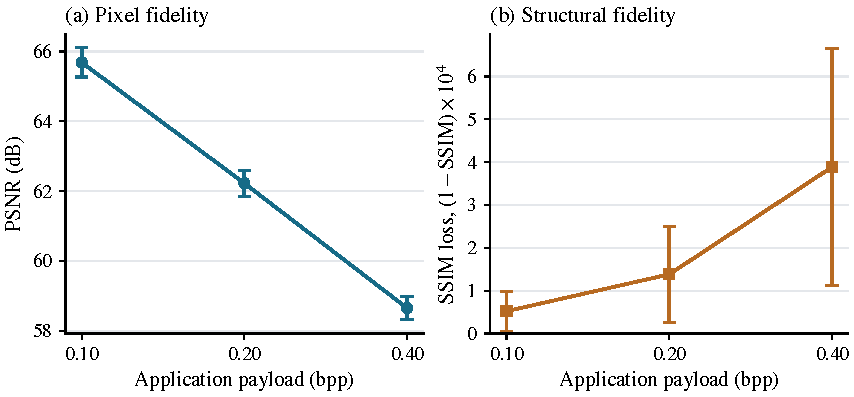
\includegraphics[width=\linewidth]{figures_revision/revised_pilot.pdf}
\caption{Independent-receiver pilot fidelity across application payloads. Points are
means and bars are between-cover standard deviations, not confidence
intervals. Lower SSIM loss means better structural fidelity. All 100
attempts at every payload recovered exactly.}
\label{fig:revised-pilot}
\end{figure}

Table~\ref{tab:revised-pilot} and Fig.~\ref{fig:revised-pilot} show the
expected payload--distortion trade-off: more embedded bits require more
pixel changes, reducing PSNR and SSIM. Structural similarity nevertheless
remains high across this pilot. Mean embedding time is approximately
$2.62$--$2.70$ s, and independent-receiver time is approximately
$0.21$ s. The three serialized JSON/base64 frames together occupy about
$350{,}485$ bytes per epoch in this fixture configuration; the absolute
size is nearly constant, so bytes per application bit decrease as payload
increases. These measurements include the declared parameter objects and
wire encoding and are not a binary-format lower bound. They quantify an
operational cost that must accompany any capacity claim.

Exact recovery here supports the implemented inverse path. It does not
estimate a deployment-wide decoding-failure probability
$\delta_{\mathsf{dec}}$, and high PSNR or SSIM does not bound the
embedding indistinguishability loss $\varepsilon_{\mathsf{emb}}$.
Image-carrier detectability is evaluated separately in
Section~\ref{subsec:hsmnet-comparison}.

\subsubsection{Sensitivity to the fusion weight}
\label{subsec:fusion-sensitivity}
To examine the fixed $\lambda=0.75$ setting, we evaluated
$\lambda\in\{0,0.25,0.50,0.75,1\}$ on 25 validation covers at each
payload, giving 375 attempts. Within a cover/payload, all variants share
the message, public context, parameter objects, masked bytes and STC seed;
receiver states are separate for these counterfactual variants. The
weight also propagates through the existing residual-feature construction.
The endpoints are therefore internal CPM variants, not standalone
MiPOD or S-UNIWARD implementations.

\begin{table}[!t]
\centering\small
\caption{Validation-only fusion sensitivity. Each cell gives mean PSNR
in dB / mean SSIM over valid outputs. Every setting has 25 attempts;
the marked cell has 24 valid outputs. No failed case was replaced.}
\label{tab:fusion-sensitivity}
\setlength{\tabcolsep}{5pt}\renewcommand{\arraystretch}{1.13}
\begin{tabular}{@{}lccc@{}}
\toprule
$\lambda$ & 0.10 bpp & 0.20 bpp & 0.40 bpp\\
\midrule
0.00 & 65.645 / 0.999957 & 62.023 / 0.999882 & 58.326 / 0.999634$^{\dagger}$\\
0.25 & 65.649 / 0.999957 & 62.077 / 0.999881 & 58.413 / 0.999650\\
0.50 & 65.642 / 0.999956 & 62.124 / 0.999880 & 58.527 / 0.999652\\
0.75 & 65.639 / 0.999953 & 62.197 / 0.999875 & 58.676 / 0.999646\\
1.00 & 65.691 / 0.999948 & 62.330 / 0.999863 & 58.871 / 0.999621\\
\bottomrule
\end{tabular}
\par\smallskip\begin{minipage}{\linewidth}\footnotesize
$^{\dagger}$One sender preflight failure at cover 2676, 0.40 bpp,
$\lambda=0$. Overall exact recovery is 374/375; the retained
$\lambda=0.75$ setting recovers 75/75. No incorrect plaintext is accepted.
\end{minipage}
\end{table}

\begin{figure}[!t]
\centering
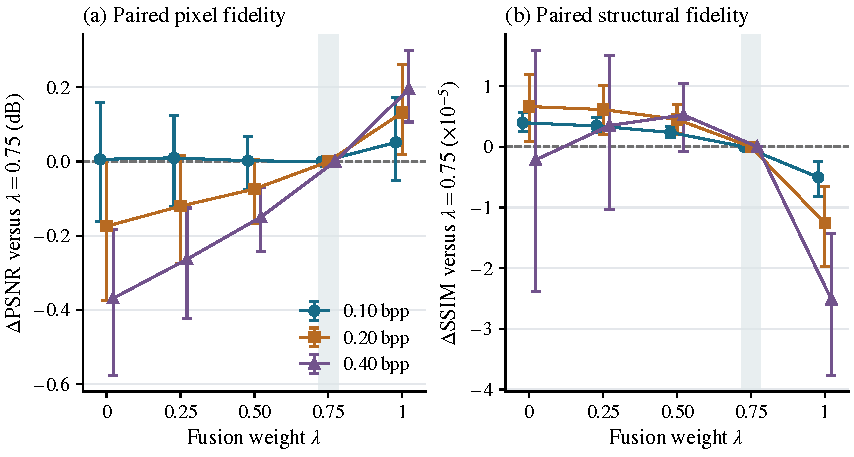
\includegraphics[width=\linewidth]{figures_revision/fusion_paired.pdf}
\caption{Paired sensitivity relative to $\lambda=0.75$. Points are mean
within-cover differences and bars are unadjusted 95\% intervals from
10,000 joint cover-bootstrap draws. Positive values favour the alternative
on the indicated metric. Each comparison has 25 common-valid covers,
except $\lambda=0$, 0.40 bpp, which has 24. The shaded band identifies the
reference weight; its paired difference is exactly zero. Horizontal
offsets separate payloads at the same weight.}
\label{fig:fusion-paired}
\end{figure}

Table~\ref{tab:fusion-sensitivity} and Fig.~\ref{fig:fusion-paired} show
that the highest mean PSNR occurs at $\lambda=1$. Relative to $0.75$,
the paired differences are $+0.052$, $+0.132$ and $+0.196$ dB across
ascending payloads. Their respective unadjusted 95\% intervals are
$[-0.051,0.172]$, $[0.020,0.263]$ and $[0.107,0.300]$ dB.
Mean SSIM is slightly lower at $\lambda=1$; the small structural
differences should not be interpreted as a demonstrated perceptual or
security advantage. Cost-construction plus embedding CPU time varies
only modestly, with group means of about $2.39$--$2.43$ s, under three
concurrent one-thread workers.

This panel quantifies distortion sensitivity around the fixed weight
$0.75$, with its observed recovery and fidelity trade-offs. It does not
establish that setting as PSNR- or security-optimal.
No detector was fitted for this panel. Consequently these fidelity
differences cannot be substituted for $\varepsilon_{\mathsf{emb}}$ in
Eq.~\eqref{eq:revised-composition}. The preflight failure also shows why
all-attempt recovery and valid-output fidelity need separate denominators.

\subsection{Stego-Object Detectability Results}
\label{subsec:detectability_results}
\subsubsection{Classical and CNN-Based Steganalysis}
\label{subsec:classical-cnn}

To examine the image-carrier detectability associated with
$\varepsilon_{\mathsf{emb}}$ in Section~\ref{sec:security}, we evaluate the image stego-object $s$
using SRM+EC, Ye-Net, and Yedroudj-Net. The adversary in this
experiment observes only the stego-object on the image channel; it
does not obtain the stego-key, the synthesised cover messages, or the
complete multichannel transcript required for message recovery.

Table~\ref{tab:detectors_payloads_test} and
Fig.~\ref{Figure_4} show that detectability is strongly
payload-dependent. At 0.10 bpp, all detectors operate close to random
classification. SRM+EC achieves 51.37\% accuracy and an AUC of
0.5444, while Ye-Net and Yedroudj-Net obtain AUC values of 0.5017
and 0.5042, respectively. This shows weak discrimination by these particular detectors at low payload. A similar pattern is observed at 0.20 bpp:
SRM+EC remains near chance with 50.53\% accuracy and AUC 0.5487,
Ye-Net obtains AUC 0.5424, and Yedroudj-Net rises only moderately
to AUC 0.5678. These observations motivate testing the lower-payload regime with stronger
wardens; they do not isolate the causal contribution of individual cost terms
or upper-bound the carrier-distribution distance.

The detection error probability $P_e$ also provides a direct link
between the empirical detector and the embedding-distance term. For an
optimal equal-prior cover--stego test, $P_e^\star=\frac{1}{2}(1-\mathrm{TV}(D_i,\mathrm{Law}(S_i)))$, so $\mathrm{TV}(D_i,\mathrm{Law}(S_i))=1-2P_e^\star$.
For a fixed detector, $P_e\ge P_e^\star$ and hence $1-2P_e\le\mathrm{TV}$ at the population level. An empirical near-chance detector therefore does not upper-bound the optimal warden or certify a small embedding loss. In the SRM+EC results,
$1-2P_e$ is approximately $0.1340$, $0.1566$, and $0.5906$ at
0.10, 0.20, and 0.40 bpp, respectively. These sample-derived values illustrate the reported detector
performance; without population-error guarantees they are not certified
bounds on the theoretical loss.

The behaviour changes at 0.40 bpp. SRM+EC reaches 79.27\%
accuracy and AUC 0.8860, while Yedroudj-Net achieves the strongest
detection performance with 82.69\% accuracy and AUC 0.9302. This
shows that, once the payload becomes large, the accumulated embedding
changes become visible to both classical residual co-occurrence features
and learned CNN features. In contrast, Ye-Net remains comparatively
weak at this payload, with 55.70\% accuracy and AUC 0.5811, suggesting
that this detector is less sensitive to the particular artefacts produced by
QIM-Fused-CF under the present training configuration.
Therefore, the strongest high-payload evidence comes from SRM+EC and
Yedroudj-Net rather than from Ye-Net.

The conditional composition bound includes a carrier-replacement loss,
but these fixed-detector measurements do not numerically instantiate it.
They show weaker observed detection at $0.10$--$0.20$ bpp and pronounced
detection at $0.40$ bpp for the component configuration specified in
Section~\ref{subsec:setup}. Supplementary
Figs.~\ref{supp-Figure_S2}--\ref{supp-Figure_S4} retain the recorded
learning trajectories. The receiver-reproducible masking/keying path is evaluated
separately with HSMNet in Section~\ref{subsec:hsmnet-comparison}; the
different configurations, cohorts and training protocols preclude a
direct detector-to-detector ranking across these two subsections.

\begin{table*}[!t]
\centering
\caption[Stego-object detectability across payloads.]
{Stego-object detectability across payloads using SRM+EC and CNN-based steganalyzers.}
\label{tab:detectors_payloads_test}
\small
\setlength{\tabcolsep}{4.3pt}

\resizebox{\textwidth}{!}{%
\begin{threeparttable}

\begin{tabular}{
@{}
l
S[table-format=1.2]
S[table-format=4.0]
S[table-format=2.2]
S[table-format=2.2]
S[table-format=1.4]
S[table-format=2.2]
S[table-format=2.2]
S[table-format=1.4]
S[table-format=2.0]
c
@{}}
\toprule
\textbf{Detector} &
{\textbf{Payload (bpp)}} &
{\textbf{Pairs}} &
{\textbf{ACC} (\%)} &
{\textbf{BACC} (\%)} &
{\textbf{AUC}} &
{\textbf{EER} (\%)} &
{\boldmath$P_e$ (\%)} &
{\textbf{MCC}} &
{\textbf{Best epoch}} &
\textbf{Subspace}\\
\midrule
\multicolumn{11}{@{}l}{\textit{Classical steganalysis}} \\
SRM+EC       & 0.10 & 1500 & 51.37 & 51.37 & 0.5444 & 46.93 & 43.30 & 0.0275 & {--} & 1000 \\
SRM+EC       & 0.20 & 1500 & 50.53 & 50.53 & 0.5487 & 47.50 & 42.17 & 0.0108 & {--} & 1000 \\
SRM+EC       & 0.40 & 1500 & 79.27 & 79.27 & 0.8860 & 20.93 & 20.47 & 0.5854 & {--} & 1000 \\
\addlinespace[2pt]
\multicolumn{11}{@{}l}{\textit{CNN-based steganalysis}} \\
Ye-Net       & 0.10 & 1999 & 50.05 & {--} & 0.5017 & 49.94 &  {--} & {--} & 80 & {--}\\
Ye-Net       & 0.20 & 1999 & 50.30 & {--} & 0.5424 & 49.69 &  {--} & {--} & 80 & {--} \\
Ye-Net       & 0.40 & 1999 & 55.70 & {--} & 0.5811 & 44.29 &  {--} & {--} & 12 & {--} \\
Yedroudj-Net & 0.10 & 1999 & 50.30 & {--} & 0.5042 & 49.69 & {--}  & {--} & 59 & {--} \\
Yedroudj-Net & 0.20 & 1999 & 54.30 & {--} & 0.5678 & 45.69 & {--}  & {--} & 79 & {--} \\
Yedroudj-Net & 0.40 & 1999 & 82.69 & {--} & 0.9302 & 17.30 & {--}  & {--} & 71 & {--} \\
\bottomrule
\end{tabular}

\begin{tablenotes}
\footnotesize
\item \textit{Notes:} ACC = accuracy; BACC = balanced accuracy; AUC = area under the ROC curve; EER = equal error rate; $P_e$ = detection error probability; MCC = Matthews correlation coefficient. Missing values indicate metrics not reported by the corresponding detector run. For SRM+EC, ``Best epoch'' is not applicable.
\end{tablenotes}

\end{threeparttable}%
}

\end{table*}




\begin{figure}[!t]
    \centering
    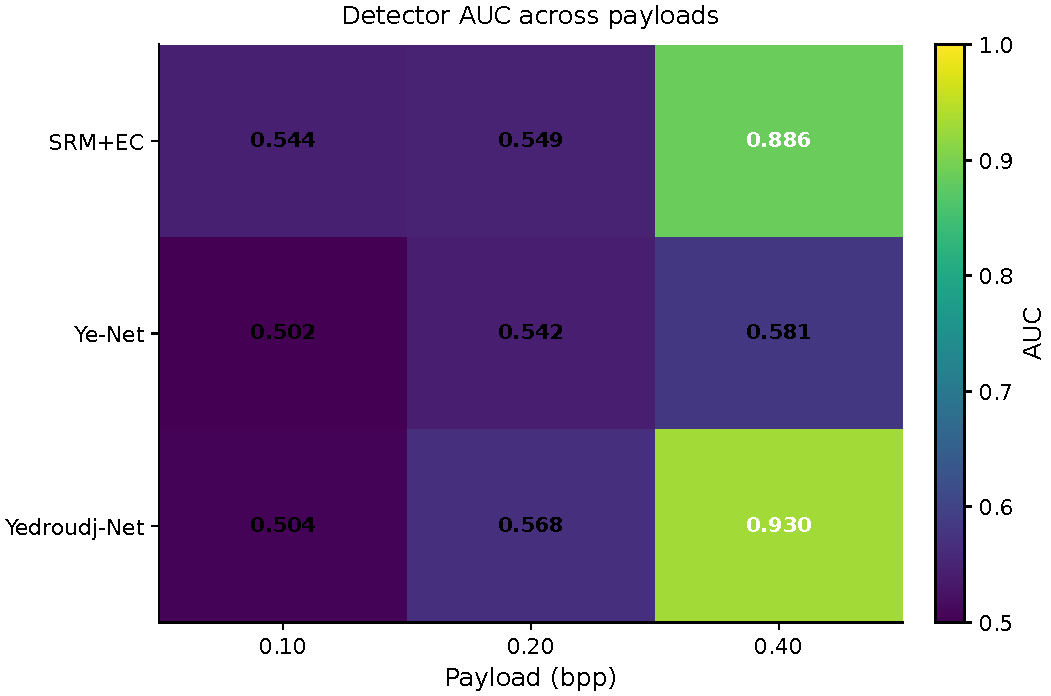
\includegraphics[width=1.0\linewidth]{Figure_2.pdf}
    \caption{Detector AUC across payloads for SRM+EC, Ye-Net, and Yedroudj-Net. Near-0.5 AUC values indicate weak cover--stego discrimination, whereas higher values indicate stronger detectability; the strongest detection occurs at 0.40 bpp.}
    \label{Figure_4}
\end{figure}




%\subsection{CNN-aware hardening}
%\textcolor{red}{This will claim: adversarial QIM should not be claimed as “universally secure”; it should be framed as CNN-aware empirical hardening. }

\clearpage
\subsubsection{Comparative Steganalysis Using HSMNet}
\label{subsec:hsmnet-comparison}
Figure~\ref{fig:matched-hsmnet} compares CPM, S-UNIWARD, the local MiPOD
approximation, WOW and HILL using the shared HSMNet observer and matched
cohort specified in Section~\ref{subsec:setup}. CPM AUCs are
0.5024/0.5054/0.5170 at 0.10/0.20/0.40 bpp. Seven of the twelve adjusted
CPM-minus-baseline intervals lie below zero: all three WOW comparisons
(differences $-0.0200/-0.0147/-0.0659$), all three MiPOD-approximation
comparisons, and S-UNIWARD at 0.40 bpp. The latter four absolute differences
are small (0.0009--0.0029); the remaining five intervals, including every
HILL comparison, contain zero. Although the AUCs are numerically close
to chance, all fifteen pointwise conditional intervals exclude 0.5;
these results establish neither equivalence nor absence of detection.
The evidence concerns image-carrier detectability, informing the
$\varepsilon_{\mathsf{emb}}$ component of
Eq.~\eqref{eq:revised-composition} for these fixed observers, implementations
and the 100-epoch budget; it does not upper-bound that loss. The
full-public-view CP-UNL evidence remains in
Section~\ref{sec:empirical_linkability}. Supplementary
Appendix~\ref{supp-sec:hsmnet-comparison} gives all numerical panels,
conditional uncertainty and provenance, while
Section~\ref{subsec:embedding_fidelity} reports the associated fidelity
trade-offs.

\begin{figure}[!htbp]
\centering
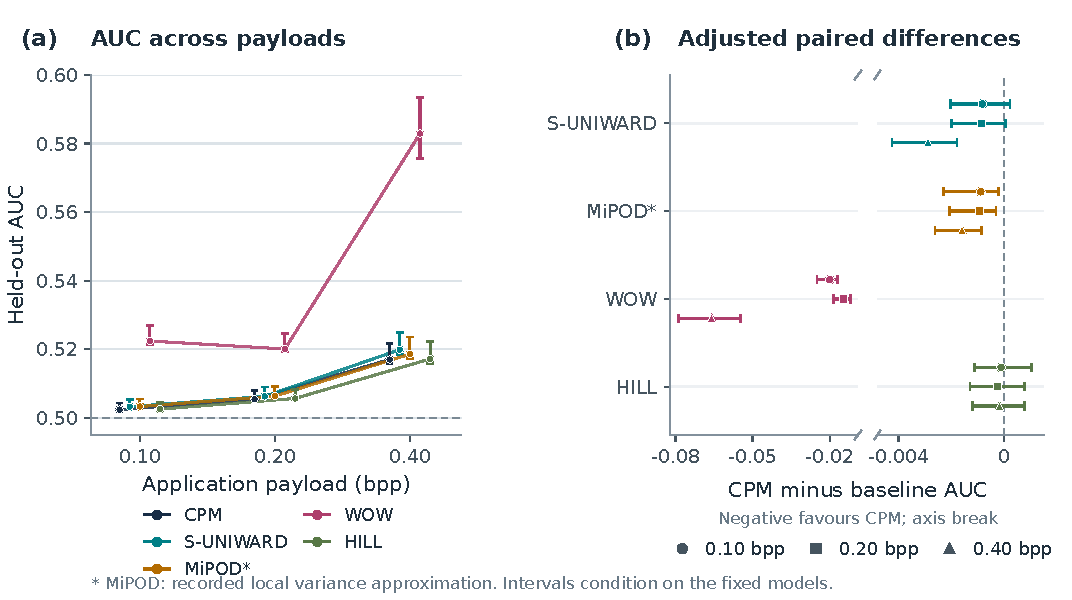
\includegraphics[width=\linewidth]{figures_revision/matched_hsmnet_comparison.pdf}
\caption{Matched five-method HSMNet evaluation. (a) AUCs and pointwise
95\% cover-bootstrap intervals; the dashed line denotes chance.
(b) CPM-minus-baseline AUC differences and twelve-way adjusted intervals;
the broken horizontal axis resolves small contrasts. Negative values
favour CPM for this fixed observer. There are 288/289/294 common-valid
test covers at 0.10/0.20/0.40 bpp; MiPOD is the local variance
approximation. Intervals condition on the saved models (Supplementary
Appendix~\ref{supp-sec:hsmnet-comparison}).}
\label{fig:matched-hsmnet}
\end{figure}

\subsection{Content Linkage and Full-Public-View CP-UNL}
\label{sec:empirical_linkability}

The linkage question differs from ordinary steganalysis. A detector asks
whether an image contains a payload; a linkage observer asks whether
public parameter content and a carrier were generated together. We first
evaluate that content association on \texttt{cpm-epoch-v2}, then
extend the observer to authentication information, public metadata and
prior queries. The second study instantiates the real-world comparison
$h=0$ in Definition~\ref{def:cp_unl}. Neither study uses the original
cover, secret keys, masks, coding seeds, hidden pair indices or file
identifiers as classifier inputs.

\subsubsection{Content-only linkage and candidate identification}
\label{subsec:revised-content-linkage}
The content study uses 300 covers, partitioned 150/50/100 for
training/validation/testing. Twelve fixed public parameter pairs and
three payloads give 10,800 native embedding attempts. Within each
cover/payload block, the message is fixed across the twelve generating
pairs. Every valid carrier is scored with its generating pair and all
eleven other candidates. Image-only and parameter-only features check
marginal balance; cross-only and combined features test association.
This is a linked-versus-wrong-candidate diagnostic: its shuffled class
excludes the generating pair, so it is not identical to the independent
sampling experiment in Definition~\ref{def:cp_unl}.

Standardised logistic regression and Extra Trees
\cite{hastie2009elements,geurts2006extremely} are fitted using balanced
class weights. Three fixed seeds are averaged for each family/view.
Validation AUC alone fixes score orientation and selects the primary
family for the combined view at each payload, before held-out scoring.
All 72 checkpoints and 24 predefined panels are retained. Three thousand
test-cover cluster bootstrap draws resample all attempted test covers
jointly across payloads and variants. Primary AUC intervals use a
Bonferroni adjustment over the three payloads; ranking and secondary
intervals are pointwise 95\%. Inference conditions on the fitted models,
fixed pair bank and complete valid blocks.

\begin{table}[!t]
\centering\small
\caption{Content-linkage primary results. Validation selected
Extra Trees at every payload. AUC intervals target 95\% family coverage
across the three payloads. Random Top-1 identification among twelve
candidates is $8.33\%$.}
\label{tab:linkability_binary_results}\label{tab:revised-content-primary}
\setlength{\tabcolsep}{4pt}\renewcommand{\arraystretch}{1.12}
\begin{tabular}{@{}lrrccc@{}}
\toprule
Payload & Test covers & Images & AUC [adjusted interval] & BACC & Top-1\\
\midrule
0.10 & 100 & 1,200 & 0.4986 [0.4963, 0.5007] & 50.00\% & 8.33\%\\
0.20 & 99 & 1,188 & 0.5012 [0.4983, 0.5041] & 50.00\% & 7.83\%\\
0.40 & 99 & 1,188 & 0.4999 [0.4967, 0.5031] & 50.00\% & 8.42\%\\
\bottomrule
\end{tabular}
\end{table}

\begin{figure}[!t]
\centering
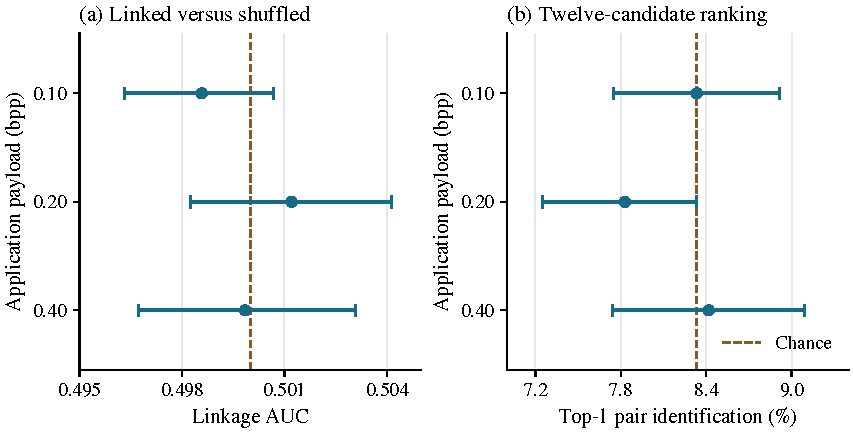
\includegraphics[width=\linewidth]{figures_revision/revised_content_linkage.pdf}
\caption{Held-out content linkage. AUC bars are adjusted primary
intervals; Top-1 bars are pointwise 95\% cover-bootstrap intervals.
Dashed lines mark their different chance references. Both tasks use
validation-frozen scores; ranking gives fractional credit for ties.}
\label{fig:linkability_combined_results}\label{fig:revised-content}
\end{figure}

There are 10,794 exact recoveries and six retained preflight failures,
with no incorrect accepted plaintext. The complete-block cohort contains
10,728 images; 66 other valid images belong to incomplete blocks and
remain in the all-attempt record. All recovered images were audited.
One training image at 0.40 bpp contains a single pixel changed from 0
to 2. Its exact recovered output is retained and disclosed; the data
therefore do not support an unconditional one-level change claim.

The primary AUCs in Table~\ref{tab:revised-content-primary} all lie close
to $0.5$, and every adjusted interval contains that reference.
Fig.~\ref{fig:revised-content} also shows that generating-pair
identification remains close to the $1/12$ ranking baseline. Marginal-only
views are exactly balanced by construction, so their chance scores are
implementation controls rather than independent secrecy evidence.
Together, the combined-feature and ranking results support weak
content association for the tested representations. They do not establish
tag privacy or bound the full CP-UNL game. The following extension tests
the broader public view directly, using a separately constructed cohort.

\subsubsection{A matched-metadata full-public-view experiment}
\label{subsec:fullview-cpunl}
The extension uses 200 disjoint covers, partitioned
100/40/60. A fresh key/session is assigned to every cover/payload block.
The parameter source is uniform over twelve declared pairs, each object
restricted to its first 65,536 bytes. These equal lengths define a
controlled conditional length stratum; the experiment does not evaluate
naturalness or generalisation to unseen parameter banks.

Before the challenge, the observer receives four public chosen-message
queries and their complete native responses. The first query is all
zero; each later message is a fixed public hash-based function of the
preceding request/response history. The challenge message is known and
all zero. For the same cover, key, epoch context and history, the native
sender produces twelve mutually exclusive challenge branches, one per
parameter pair. These are alternative worlds, not twelve live
transmissions with reused nonces. An observer receives one challenge.
Four history attempts plus twelve challenge attempts for each of 600
blocks give 9,600 native attempts.

Write $\Gamma_j=(\gamma_1^{(j)},\gamma_2^{(j)})$ and let $s_j$ be its
native carrier in a fixed block. The two content distributions are
\[
 (\Gamma_J,s_J),\qquad
 (\Gamma_J,s_K),\quad J,K\stackrel{\$}{\leftarrow}\{1,\ldots,12\}
 \text{ independently}.
\]
Thus the linked world has twelve equiprobable branches; the independent
world has all 144 pair/carrier combinations, \emph{including} the twelve
diagonal combinations $J=K$. Keeping that overlap is necessary for the
same-marginal independent comparison. Context, visible lengths and prior
history match between the worlds. The laboratory challenger uses the
native authentication function to generate a valid HMAC for each actual
canonical transcript. These independent-content views are challenge
distributions, not attacker-generated forgeries or claimed correct
encodings of the known message.

The complete observer record contains every challenge-frame byte,
session/epoch/header/nonces, lengths, version, codec and actual tags,
together with all four query messages and full responses. Classifiers
use fixed public feature maps of this record: content statistics,
whole-object byte sketches, raw public context and tag features, ordered
query/response representations and cross-history comparisons. Complete
raw views remain reconstructible. Five predefined views are evaluated:
metadata-only, content-only, authentication-only, full challenge and
full history. Logistic regression and Extra Trees with three seeds give
90 saved models and 30 panels. The primary full-history family and
orientation are selected using validation alone. Held-out data are
scored once; the test set is not used to revise features or selection.

\begin{table}[!t]
\centering\small
\caption{Full-public-view CP-UNL extension: validation-selected
full-history results. AUC intervals are adjusted over three primary
payload tests. The gap is the fixed rule's TPR minus FPR, not a bound
over all observers. LR = logistic regression; ET = Extra Trees.}
\label{tab:fullview-primary}
\setlength{\tabcolsep}{4pt}\renewcommand{\arraystretch}{1.12}
\begin{tabular}{@{}llrccc@{}}
\toprule
Payload & Family & Test covers & AUC [adjusted interval] & BACC & Gap\\
\midrule
0.10 & LR & 60 & 0.5023 [0.4824, 0.5210] & 51.43\% & 0.0286\\
0.20 & ET & 60 & 0.5119 [0.4926, 0.5311] & 50.00\% & 0.0000\\
0.40 & ET & 59 & 0.4905 [0.4715, 0.5096] & 50.00\% & 0.0000\\
\bottomrule
\end{tabular}
\end{table}

\begin{figure}[!t]
\centering
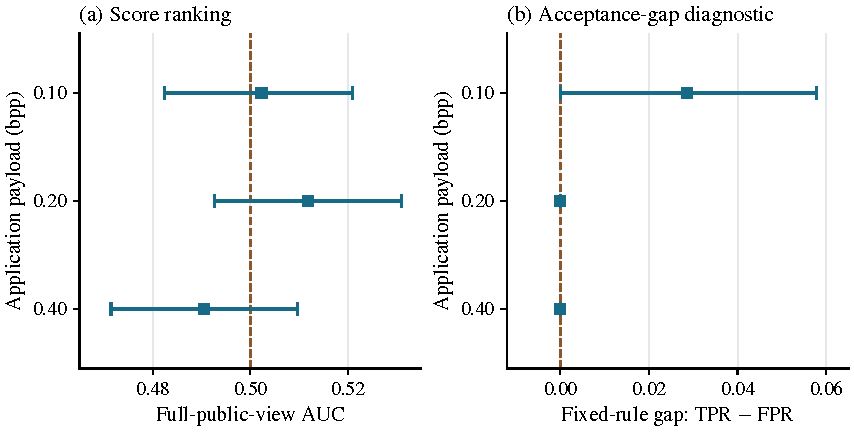
\includegraphics[width=\linewidth]{figures_revision/fullview_cpunl_primary.pdf}
\caption{Full-public-view CP-UNL diagnostics with four prior queries.
Panel (a) shows primary AUCs with adjusted cover-cluster intervals;
panel (b) shows signed acceptance gaps with pointwise 95\% intervals.
The reference is $0.5$ for AUC and zero for the gap. Zero gaps for the
two ET rules reflect constant decisions at threshold $0.5$; their AUCs
still measure score ranking.}
\label{fig:fullview-cpunl}
\end{figure}

Of 9,600 attempts, 9,572 recover the exact plaintext and 28 fail sender
preflight; none releases incorrect accepted plaintext. Four incomplete
blocks are removed symmetrically from both worlds. This leaves 596
blocks and 92,976 public views; 36 other valid native outputs remain
outside the primary cohort. No recovered image in this extension has
a pixel change exceeding one level. Independent verification checks
every world's HMAC, canonical/wire/observer hashes, matched metadata,
conditional marginals and query history, and reproduces every held-out
prediction from all 90 saved checkpoints.

\paragraph{Results and their connection to CP-UNL.}
At 0.10 bpp, full-history AUC is $0.5023$; at 0.20 bpp it is $0.5119$;
at 0.40 bpp it is $0.4905$. Every adjusted interval in
Table~\ref{tab:fullview-primary} contains $0.5$. The results therefore
provide favourable empirical support for the matched-public-view CP-UNL
objective at all three tested payloads. They do not demonstrate equality
of the distributions: the intervals also admit small departures from
chance. The full-view intervals are wider than the content-only intervals,
and the studies differ in covers, parameter lengths, histories and tasks;
their scores should not be pooled or treated as a paired comparison.

For a fixed decision rule $f$, the empirical game-related quantity is
\begin{equation}\label{eq:empirical_cp_unl_adv}
\widehat g_f=
\widehat{\Pr}[f(V^0_{\mathsf{link}})=1]
-\widehat{\Pr}[f(V^0_{\mathsf{ind}})=1]
=\widehat{\mathrm{TPR}}-\widehat{\mathrm{FPR}}.
\end{equation}
Its absolute value is the acceptance-gap diagnostic corresponding to
Definition~\ref{def:cp_unl}; equal-prior balanced accuracy satisfies
$|\widehat g_f|=|2\widehat{\mathrm{BACC}}-1|$. AUC instead measures
ranking across thresholds and is not this gap. At 0.10 bpp the fixed
rule has signed gap $0.0286$, with a pointwise interval extending from
approximately $-0.000006$ to $0.05787$. At the other payloads the selected
ET rules make constant decisions at threshold $0.5$, giving zero gap;
this does not imply that every threshold or observer has zero advantage.

Two secondary pointwise intervals exclude chance: authentication-only
ET at 0.20 bpp gives AUC $0.5255$ $[0.5080,0.5427]$, and content-only LR
at 0.10 bpp gives $0.4979$ $[0.4959,0.4996]$. These are exploratory
findings among 30 predefined panels, without simultaneous adjustment.
They remain reported rather than being dismissed as established random
variation or used to reorient a model after testing. Supplementary
Section~\ref{supp-sec:revision-details} reports every panel.

Metadata-only AUC is exactly $0.5$ because metadata match by design.
A separate synthetic control places a publicly computable parameter
digest prefix in the carrier and processes it through the same public
feature maps. Both classifier families attain AUC $23/24=0.9583$, the
maximum under the independent world's diagonal overlap. This confirms
sensitivity to that implanted linkage, not to every possible leakage.

The experiment aligns with the \emph{real-world} $h=0$ comparison in
Definition~\ref{def:cp_unl}. Lemma~\ref{lem:cpunl}, by contrast, uses
the content/tag transition after key separation and uniform-mask
replacement and retains the stated replacement losses. Accordingly,
these measurements are not estimates of $\varepsilon_{\mathsf{unl}}$
and do not certify its premises. They strengthen the evidence for the
implemented conditional public-view objective while preserving the
general conditional guarantee in Eq.~\eqref{eq:revised-composition}.
The remaining scope is explicit: a finite pair bank, fresh block keys,
one four-query policy, fixed feature/classifier families and complete
valid blocks. Network timing, active decryption queries and
failure/availability linkage are outside this experiment; public headers
continue to identify the intended channel association.


\subsection{Timed Active Attacks and Authenticated Recovery}
\label{subsec:multichannel_robustness}
\label{subsec:revised-active}

The active experiment tests the implementation paths underlying the
replay and substitution analysis and the delivery premise of
Lemma~\ref{lem:resync}. Thirty saved real-image epochs from ten pilot
covers, spanning all three payloads, are subjected to eleven scenarios,
two window/timeout profiles and five seeds, producing 110 traces.
A separate receiver consumes frame bytes and virtual arrival times
with the shared configuration, session, secret and protected state.
Attack labels, source covers and expected plaintext are available only
to the evaluator, which compares each actual accepted plaintext and
canonical transcript with the authorised fixture.

The profiles are $(W,T)=(3,200\,\mathrm{ms})$ and
$(5,400\,\mathrm{ms})$. Both use 100 ms epoch spacing, maximum
cross-channel skew of 100 ms, two candidate frames per channel/epoch,
an 8 MiB serialized-frame budget and 128 cached failed triples per
epoch. A declared shared epoch clock advances the receive window;
packet arrival does not advance it. No ECC or heartbeat recovery is
assumed. The full event and skip policy is specified in Supplementary
Section~\ref{supp-sec:revision-details}.

\begin{table}[!t]
\centering\small
\caption{Timed active-attack outcomes, summed over the two profiles and
five seeds (ten correlated traces per row). Each row offers 300 epoch
events. Both profiles have the same per-scenario delivery counts. All
unauthorised, incorrect-plaintext and repeated acceptances are zero.}
\label{tab:active-window-results}
\setlength{\tabcolsep}{4pt}\renewcommand{\arraystretch}{1.1}
\begin{tabularx}{\textwidth}{@{}>{\raggedright\arraybackslash}Xrrr@{}}
\toprule
Scenario & Exact recovery & Erasures & Invalid MACs rejected\\
\midrule
Honest delivery & 300 & 0 & 0\\
Bounded reordering & 300 & 0 & 0\\
Burst delay & 260 & 40 & 0\\
Burst suppression & 260 & 40 & 0\\
Persistent C2 suppression & 0 & 300 & 0\\
Accepted-epoch replay & 300 & 0 & 0\\
Tampering and splicing & 300 & 0 & 160\\
Bounded injection flood & 300 & 0 & 7,480\\
Feedback-driven injection & 300 & 0 & 364\\
Malformed frames & 300 & 0 & 0\\
State reload and replay & 300 & 0 & 0\\
\midrule
Total & 2,920 & 380 & 8,004\\
\bottomrule
\end{tabularx}
\end{table}

\begin{figure}[!t]
\centering
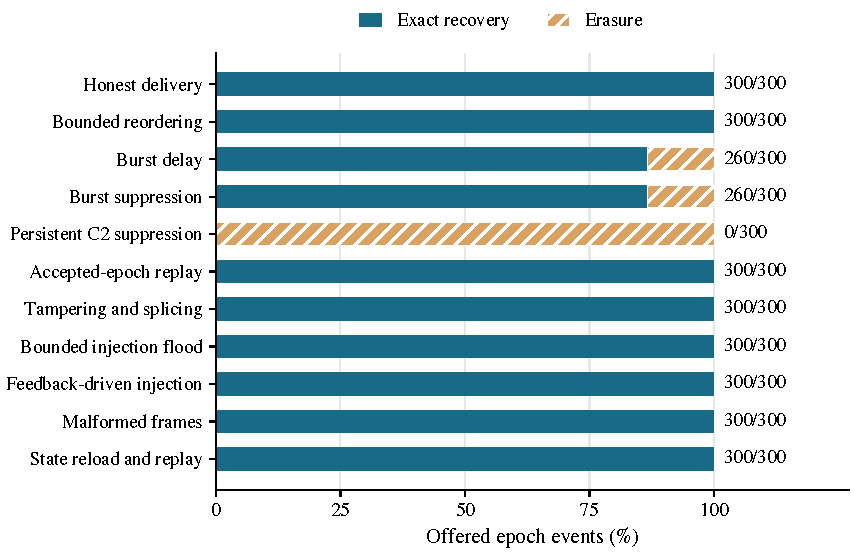
\includegraphics[width=\linewidth]{figures_revision/active_attack_delivery.pdf}
\caption{Delivery and erasures under active interference. The fraction
of offered epoch events is shown for each scenario; labels give exact
recoveries out of 300 opportunities. Erasures represent unavailable or
ineligible authentic triples, not incorrectly accepted plaintext.
These are correlated finite traces, so no population confidence interval
is attached to the bars.}
\label{fig:active-window-delivery}
\end{figure}

Across 3,300 offered epoch events, 2,920 recover exactly and 380 are
erased (Table~\ref{tab:active-window-results}). There are no unauthorised
transcript acceptances, incorrect accepted plaintexts or repeated epoch
acceptances. The receiver performs 10,924 full authentication attempts,
rejects 8,004 incorrect MACs before decoding, and invokes native
extraction exactly once per accepted epoch. Front-end, freshness, skew
and timeout rejections are separately recorded; a zero invalid-MAC
count does not imply that no malicious frame was rejected.

Fig.~\ref{fig:active-window-delivery} separates integrity from
availability. Persistent C2 suppression prevents every complete epoch,
while burst delay or suppression removes four epochs in each affected
trace. In the delay case, C2 exceeds the common 100 ms skew limit even
under the 400 ms timeout; a longer timeout alone does not make those
triples eligible. After the disruption, all 18 clean-tail epochs in
each of the 20 affected traces recover, giving 360/360 clean-tail
recoveries. The first clean-tail epoch completes 29--35 ms after its
scheduled send. These are virtual arrival delays, excluding CPU service
and queueing.

The rejection behaviour is consistent with the authenticated transcript
boundary used in the replay and MitM arguments: an invalid complete
transcript does not reach the image decoder or update accepted-epoch
state. Peak retained serialized-frame storage is 1,401,055 bytes and
the peak candidate count is nine, both within the configured caps.
These are transient-buffer measurements, not total process memory;
protected replay state is separate and reaches 4,426 bytes. The
state-reload scenario restores saved epoch/nonce sets in the same
receiver process, clears transient buffers and rejects recorded accepted
traffic. It is not a process-crash, storage-rollback or concurrent-state
qualification.

These observations support the tested authentication, freshness,
reconstruction and bounded-state paths in
Eq.~\eqref{eq:combined-mc-security-bound}. They do not estimate MAC-forgery
probability or universal decoder/state failure rates. The repeated
fixtures and seeded traces are correlated; the aggregate delivery ratio
is not a real-network population estimate. Flooding has a finite fixed
budget before legitimate arrivals, and the two profiles vary window
and timeout together. Delivery therefore remains conditional on usable
authentic opportunities, as required by Lemma~\ref{lem:resync}.

The 36-epoch/540-candidate deterministic authentication checks
remain in Supplementary Section~\ref{supp-sec:legacy-transport} as
regression evidence. The synthetic loss/jitter/ECC abstraction is retained
there separately; its synthetic C3 objects and assumed erasure recovery
must not be combined with the present real-image authenticated results.


\subsection{Masking Ablations}
\label{subsec:masking_ablations}

The original-feature sender-side mask generator was evaluated separately from
image embedding by
varying the public cover feature $\psi(\cdot)$, the relative QIM step
$\Delta/\Delta_0\in\{0.5,1,2\}$, and the dither source. For the all-zero
message, $b=\mu$, so the experiment directly measures the generated mask.
Across the $33$ configurations and payloads of $0.10$, $0.20$, and
$0.40$~bpp, the absolute bit bias remained within
$[0.0011,0.0027]$, empirical min-entropy remained within
$[0.9922,0.9968]$ bits per output bit, and monobit/runs pass rates were
$98$--$100\%$ and $96$--$100\%$, respectively. The small differences among
feature maps, QIM steps, and dither controls indicate that the observed mask
statistics are stable under the tested parameter changes.

A leave-one-seed-out logistic warden was also trained to distinguish masked
payload windows from independent uniform controls. Over all $165$ settings,
mean accuracy was $0.5004$, mean AUC was $0.4993$, and the mean normalised
proxy
\begin{equation}
 \widehat{\varepsilon}_{\mathsf{param}}^{\mathsf{clf}}
 =
 2\left|\widehat a-\frac12\right|
\end{equation}
was $0.0291$ (maximum $0.0933$). For the reference configuration
($\psi=\textsf{HashID}$, cover-conditioned PRF dither, and
$\Delta=\Delta_0$), the corresponding mean accuracy, AUC, and proxy were
$0.5058$, $0.5037$, and $0.0297$. These are classifier-dependent observations of the original-feature generator.
They are neither evaluations of the received-field mask nor upper
bounds on its computational masking loss or statistical TV distance.

A separately recorded component configuration additionally achieved mean BER
$1.102\times10^{-3}$ and $99.71\%$ exact recovery over $10{,}000$ images at
$0.30$~bpp. This result supports practical extraction but is not claimed for
every ablation or payload. Full configuration-wise results, message-class
comparisons, recovery limitations, and the relationship to
$\varepsilon_{\mathsf{emb}}$ and
$\varepsilon_{\mathsf{sched}}(\sigma^\star)$ are reported in
Supplementary Appendix~\ref{supp-subsec:masking_ablations}.

%\subsection{Multichannel Robustness}
%Emulate $\Sigma$: losses, jitter, skew; window $W$, timeout $\tau$, skew $\Delta$, heartbeat $h$, ECC $(n,k,t)$. Report re-sync success, delay (compare with Lemma~\ref{lem:resync}), integrity failures (expected $\approx 0$).

%\subsection{Scheduling Footprint}
%Measure $\varepsilon_{\mathsf{sched}}$: KS/MMD between cover and stego inter-arrival distributions; show small gaps under admissible shaping.

%\subsection{Overheads and Runtime}
%Per-epoch bytes (headers, nonces, MAC), T$_{\mathrm{enc}}$/T$_{\mathrm{dec}}$ on stated hardware.








\subsection{Comparison with Recent Steganography and Steganalysis}
\label{subsec:recent-comparison}

\subsubsection{Complementary roles and architectural novelty}
CPM formalises \emph{Steganography by Cover-Parameterised Modification}
through the complementary roles of synthesis and cover modification.
Message-independent synthesis supplies public cover-parameter objects;
keyed, parameter-conditioned masking protects the message; and adaptive
modification places the masked bits in an existing cover. Synthesis can
therefore be tailored to the contextual objects' benign distribution,
while the carrier encoder controls the distortion needed to realise the
payload. In the image instantiation, this division connects text-valued
parameters to native-resolution image embedding through a reproducible
bitstream interface. The receiver extracts the masked bits and reconstructs
the mask from authenticated received fields, without requiring the original
image or sender-side cost map.

The formal contribution is this synthesis--masking--modification
construction together with its authenticated multichannel composition
(Sections~\ref{Hybrid_stego_model}--\ref{sec:security}). CP-IND and CP-UNL
make the appearance and content linkage of public parameters explicit;
IND-STEGO-MC additionally accounts for the carrier and joint transport
view; and MC-ATTACK treats active interference and receiver acceptance.
The separate loss terms identify how sampler quality, keyed masking,
adaptive embedding, scheduling, authentication and receiver state
contribute to the resulting conditional guarantees. This gives the complementary
components defined interfaces and testable responsibilities.

\subsubsection{Relationship to recent generative constructions}
Recent methods demonstrate several effective ways to make synthesis carry
the secret. MDDM maps message bits into Gaussian noise using a pre-shared
Cardan grille, generates the image by diffusion, and recovers the message
through inversion \cite{xu2025mddm}. Yuan \emph{et al.} use an adaptive
distribution-preserving mapping into Gaussian latent variables
\cite{yuan2026provably}. Zhang \emph{et al.} combine locally normalised
orthogonal mapping with stable-diffusion inversion
\cite{Zhang2026MappingDiffusion}. These approaches develop the
message-to-generation path. CPM introduces a complementary path in which
the synthesized objects provide message-independent public context and
the payload is embedded by modifying a selected existing carrier.
Consequently, its current receiver uses carrier extraction and mask
reconstruction rather than inversion of a payload-bearing diffusion image.
This supports the use of established image sources and distortion-based
coding within the formal CPM interface.

Qi \emph{et al.} combine autoregressive image steganography with auxiliary
stego text for recovery after lossy image processing
\cite{qi2025provably}. Their construction shows the value of coordinating
different media for robustness. CPM uses modality diversity for a different
purpose: its two public parameter objects condition the keyed mask, while
complete-epoch authentication binds them to the image and reconstruction
context. Qi \emph{et al.} and Yuan \emph{et al.} also provide
provable-security arguments. CPM's distinctive contribution is the
specified synthesis--modification architecture and the joint treatment of
parameter linkage, carrier observations, transport, and authenticated
receiver state in its compositional model.

\subsubsection{Practical significance and supporting evidence}
CPM's modular construction permits the parameter sampler and carrier
encoder to be assessed separately, then checked together at the receiver.
The classical baselines in Section~\ref{subsec:setup} serve this purpose:
WOW, S-UNIWARD, HILL and MiPOD compare adaptive image embedding under common
covers and target payloads. Cover-stream probes examine the synthesized
context, while image fidelity, detectability and linkage probes examine
the carrier and its relationship to that context
(Sections~\ref{subsec:cover_stream_naturalness}--\ref{subsec:multichannel_robustness}).
The component results identify $0.10$--$0.20$ bpp as a promising
operating region for the tested image configuration, combining high
structural fidelity with weak discrimination by the recorded detectors.

The complete-protocol studies demonstrate that the formal interfaces are executable
and can be evaluated separately. The independent receiver recovers all
300 pilot epochs; the weight panel reports 374/375 exact recoveries and
the observed fidelity sensitivity without claiming an optimal weight.
The content and full-public-view studies assess parameter--carrier
association on separate cover cohorts, with metadata, native tags and
four prior queries included in the latter. Their favourable primary
scores are empirical evidence for the declared CP-UNL comparison, not
a universal advantage bound. Finally, the 110 timed traces check
authentication, freshness and recovery under explicit interference,
including delivery loss under complete channel suppression.
These complementary measurements support CPM's integration of synthesis,
receiver-reproducible masking, adaptive modification and authenticated
multichannel operation. They preserve the distinction between image
fidelity, detection, linkage and active acceptance rather than using
one metric as a substitute for another.

\subsubsection{Recent steganalysis and matched evaluation}
Recent detectors provide complementary ways to examine the carrier layer.
SRNet learns noise residuals with minimal handcrafted constraints
\cite{Boroumand2019SRNet}. PSDR-SNet uses region-sensitive partitioning and
Siamese similarity learning to examine potential steganographic-signal
differences \cite{Su2025PSDRSNet}. HSMNet combines local convolutional
features, hybrid dilated convolution and attention for multi-resolution
grayscale steganalysis \cite{Yang2026HSMNet}. Their residual, regional and
multi-resolution perspectives are relevant to QIM-Fused-CF's
texture-sensitive allocation of image changes. CPM's separation of
carrier distinguishability from plaintext confidentiality and
authenticated acceptance allows these detectors to evaluate the embedding
component without conflating the three security objectives.

Table~\ref{tab:rw-compare} and its
\hyperref[tab:rw-quantitative]{quantitative continuation} place the
steganographic constructions and their published evidence in context. A matched
experimental comparison should fix cover identities, net payload,
resolution/preprocessing, channel transformations and detector training,
with validation-based model selection and held-out evaluation. Generative
methods additionally require benign images from the same generator;
PSDR-SNet's downsampled BOSSBase setting must likewise be aligned with
native-resolution runs. Section~\ref{subsec:hsmnet-comparison}
reports the completed matched HSMNet comparison across CPM and four
spatial baselines, with full settings and implementation qualifications
in Supplementary Appendix~\ref{supp-sec:hsmnet-comparison}. Published
external scores retain their own settings; no CPM experiment is attributed
to SRNet or PSDR-SNet. The HSMNet results address the image-carrier
component, while Section~\ref{sec:empirical_linkability} evaluates
full-public-view CP-UNL separately.

\subsubsection{Native generative comparison with Pulsar}
\label{subsec:native-pulsar}
Pulsar provides a published generative comparator with a provable-security
construction for diffusion-model outputs \cite{Jois2024Pulsar}.
We compare the executable implementations at the same application-message
lengths while retaining their native carriers and benign sources.
Figure~\ref{fig:native-pulsar} presents the principal outcomes; complete
tables and reproducibility details appear in Supplementary
Section~\ref{supp-sec:native-comparisons}.

CPM recovered all 600 messages. Pulsar recovered 185/200, 180/200 and
153/200 at 128, 256 and 384 bytes, respectively. The 54 native capacity
failures and 28 other native failures remain in these denominators.
This establishes an observed recovery advantage for CPM in the fixed
configuration. Its primary content-detection AUCs were 0.5002, 0.5043
and 0.4963, compared with Pulsar's 0.5445, 0.5251 and 0.6035.
All three payload-adjusted intervals for the between-method AUC
differences include zero, so these measurements support weak
discrimination of CPM by the tested observers without establishing
detectability superiority. The detector comparisons use the same
successful source groups for both methods; recovery results retain
every attempt.

Pulsar uses fewer serialized bytes in this panel: approximately
378--380\,kB per exactly recovered message, compared with CPM's
525\,kB including the two public objects and three authenticated frames
($1\,\mathrm{kB}=1{,}000$ bytes). These costs expose a practical trade-off
between the native synthesis primitive and CPM's complete epoch service.
The detector scores examine the carrier contribution associated with
$\varepsilon_{\mathsf{emb}}$ in Eq.~\eqref{eq:revised-composition};
they are finite-observer measurements against each method's benign
source. Pulsar's single-carrier interface has no CPM-style public-parameter
CP-UNL score; the corresponding CPM evidence remains the separate
experiment in Section~\ref{sec:empirical_linkability}.

\begin{figure}[!t]
\centering
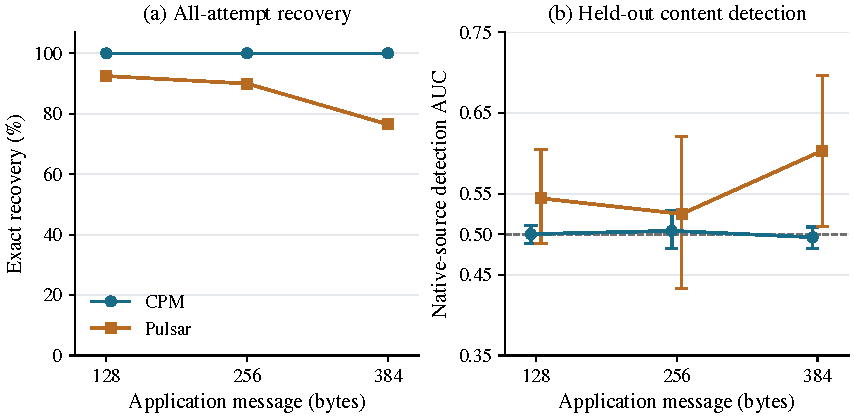
\includegraphics[width=\textwidth]{figures_revision/native_pulsar_comparison.pdf}
\caption{Native generative comparison at matched application-message
lengths. (a) Exact recovery over 200 attempts per method and length,
including every capacity or decoding failure. (b) Content-detection AUC
against each method's native benign source, with pointwise 95\%
source-group bootstrap intervals. Source groups were split
100/40/60 for training/validation/test; common successful test cohorts
contain 55/53/45 groups. Model family, tuning, orientation and threshold
were selected using validation only. Carriers retain their native
formats. Full cost and adjusted-contrast tables are in Supplementary
Section~\ref{supp-sec:native-comparisons}.}
\label{fig:native-pulsar}
\end{figure}

\subsubsection{Local distributed-message comparison with Assemblage}
\label{subsec:native-assemblage}
Assemblage combines generative carriers with perceptual-hash discovery
and rateless erasure coding for distributed messages
\cite{Jois2026Assemblage}. We evaluate its native local message path
against CPM at 1,024, 2,048 and 4,096 application bytes.
Without added erasures, CPM recovered 10/10 messages at every length;
Assemblage recovered 6/10, 5/10 and 4/10.
Across its 310 candidate packets, the original capacity gate skipped
71 candidates and 18 transmitted carriers produced decoder exceptions.
These outcomes describe the recorded implementation and fixed
configuration, with every candidate retained in the accounting.

Figure~\ref{fig:native-distributed} shows higher observed CPM recovery
at every tested per-object erasure probability. Both methods lose
delivery as erasures increase; at probability 0.30, CPM recovers
30--38\% of traces, consistent with its requirement to receive all
three frames. Mean transmitted bytes over all attempts are approximately
0.525\,MB for CPM and 1.360/2.663/5.057\,MB for Assemblage at the three
message lengths, with offline state and hash-bank costs reported separately.
Thus, this panel favours CPM in observed delivery and serialized
communication cost. Its ten source groups per length and different
native object sizes delimit that comparison.

These observations test the delivery/correctness side of the receiver
contract underlying MC-ATTACK (Section~\ref{sec:integrity}): missing
objects may prevent delivery even when acceptance checks remain intact.
The erasure panel complements the timed active-attack study; it does
not measure forgery probability, scheduling anonymity or deployed
network performance. Together, the two native comparisons add
quantitative evidence for CPM's executable synthesis--modification
architecture while keeping recovery, detection, communication cost and
cryptographic guarantees distinct.

\begin{figure}[!t]
\centering
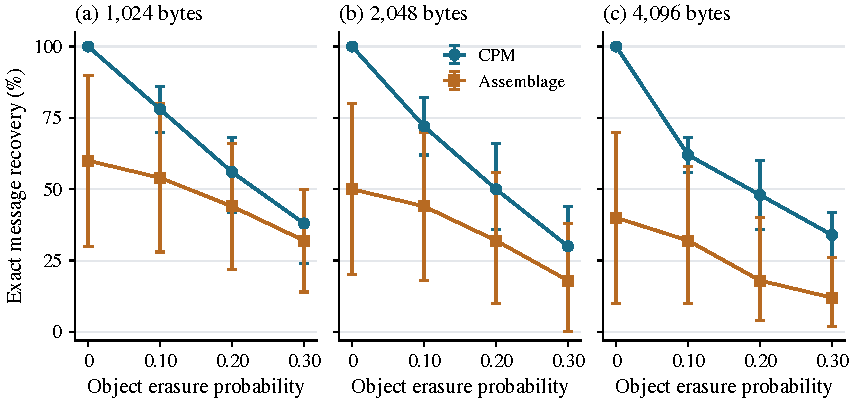
\includegraphics[width=\textwidth]{figures_revision/native_distributed_comparison.pdf}
\caption{Local distributed-message recovery at (a) 1,024, (b) 2,048 and
(c) 4,096 application bytes. Each method uses ten fixed source/message
groups per length. Saved native outcomes are replayed under independent
per-object erasure probabilities 0, 0.10, 0.20 and 0.30 with five seeds;
an object is a CPM frame or an Assemblage image. Bars are pointwise
95\% bootstrap intervals clustered by source group. Zero-loss seeds
repeat the same intact transmission; a collapsed interval at 10/10
is not population-perfect reliability. Native capacity skips and decoder
exceptions remain included. Full delivery and cost tables appear in
Supplementary Section~\ref{supp-sec:native-comparisons}.}
\label{fig:native-distributed}
\end{figure}

\subsection{Evidence and Scope of the Security Claims}
\label{subsec:empirical-security-bridge}

The experiments follow the modular structure of
Eq.~\eqref{eq:revised-composition} and the active bound in
Eq.~\eqref{eq:combined-mc-security-bound}. Table~\ref{tab:empirical-security-map}
summarises this connection. The two linkage studies answer progressively
broader empirical questions: the first tests parameter--carrier content
association, and the second adds the complete public authentication,
context and four-query history for the declared $h=0$ worlds. Their
favourable primary results support those tested objectives; neither
changes the quantifier over permitted efficient observers in the formal
definition. In particular, a confidence interval containing chance is
not an equivalence test or a numerical upper bound on a hybrid loss.

\begin{table}[!t]
\centering\small
\caption{Connection between measurements and the conditional security
model. Each measurement retains its source version and experimental scope.}
\label{tab:empirical-security-map}
\setlength{\tabcolsep}{4pt}\renewcommand{\arraystretch}{1.12}
\begin{tabularx}{\textwidth}{@{}>{\raggedright\arraybackslash}p{.21\textwidth}>{\raggedright\arraybackslash}p{.27\textwidth}>{\raggedright\arraybackslash}X@{}}
\toprule
Security component & Measurement & Interpretation\\
\midrule
CP-IND; sampler mismatch & Recorded MAUVE, RoBERTa, lexical/POS probes & Resemblance to selected benign corpora; not a bound over all distinguishers.\\
\addlinespace
Correctness; $\delta_{\mathsf{dec}}$ & 300-epoch pilot, 375 weight trials, native linkage recovery audits & Checks the actual inverse path; failures remain in all-attempt accounting.\\
\addlinespace
Carrier; $\varepsilon_{\mathsf{emb}}$ & Complete-protocol fidelity, matched HSMNet AUCs/paired contrasts (Section~\ref{subsec:hsmnet-comparison}), native-source probes and component detectors & Completed HSMNet comparison supports seven adjusted relative differences; five remain unresolved. Finite, fixed-observer evidence does not upper-bound the carrier-replacement loss.\\
\addlinespace
CP-UNL; $h=0$ & Content ranking and full-public-view classification & Tests declared finite observers and histories; does not estimate the H2 transition $\varepsilon_{\mathsf{unl}}$.\\
\addlinespace
Active acceptance and state & 110 timed traces; exact plaintext, rejection and replay checks & Supports tested MAC/freshness/decoder paths; not cryptographic forgery or population failure probabilities.\\
\addlinespace
Scheduling; $\varepsilon_{\mathsf{sched}}(\sigma^\star)$ & Recorded KS/MMD/timing probes & Describes the simulated trace model; neither authenticated delivery nor marginal agreement bounds the complete scheduling loss.\\
\bottomrule
\end{tabularx}
\end{table}

Lemma~\ref{lem:cpunl} retains content and tag-privacy premises after
key/mask replacement. The real-world extension evaluates the intended
public-view comparison without proving those premises negligible for
every adversary. Similarly, zero incorrect acceptances in the active
traces does not determine $\varepsilon_{\mathsf{mac}}(Q,q_v)$,
$\delta_{\mathsf{fresh}}$ or $\delta_{\mathsf{state}}$. Key derivation,
PRF security and protected state retain their stated assumptions.
Empirical AUCs, rejection counts and timing tests therefore should not
be added together as a numerical instantiation of the security bounds.

For classifier metrics, the full-view experiment uses the direct
fixed-rule gap in Eq.~\eqref{eq:empirical_cp_unl_adv}. Component detector
tables retain their recorded metric conventions: the reported SRM+EC
accuracy and $P_e$ are distinct summaries and are not complements.
AUC is a ranking measure, and $2|a-1/2|$ converts an equal-prior
accuracy from one fixed rule only. These distinctions preserve the
link between the experiments and their actual formal objectives.


\section{Conclusion}
\label{sec:conclusion}

This paper introduced a cover-parameterised multichannel hybrid
steganographic framework that combines message-independent
cover-parameter synthesis with adaptive cover modification. The
framework formalises cover-parameter indistinguishability and
unlinkability, multichannel trace indistinguishability, and active
confidentiality and integrity under full cross-channel observation
and manipulation. Its protocol integrates receiver-reproducible
parameter-conditioned masking, QIM-Fused-CF embedding,
authenticated epoch binding, bounded scheduling, and
re-synchronisation. The component detectors in
Section~\ref{subsec:classical-cnn} show weaker discrimination at lower
payloads and substantially greater exposure at 0.40 bpp. The separate
matched HSMNet study in Section~\ref{subsec:hsmnet-comparison} evaluates
the complete-protocol carrier directly, with CPM AUCs of 0.5024/0.5054/0.5170.
These configuration-specific results do not establish payload-independent
security or a bound against other wardens.
The analysis identifies separate conditions for synthesis, masking,
embedding, scheduling, authentication and receiver state. The experiments
exercise their interfaces within the declared configurations; they do not
establish secure deployment under arbitrary traffic or interference.

Practical deployment must preserve the conditions of this composition.
The current epoch tag authenticates the complete encoded carrier bytes.
Recompression, resizing or other byte-changing channel operations therefore
invalidate that tag unless the original authenticated bytes are restored
before verification. Robust extraction alone would not make a changed
carrier acceptable. A deployment allowing such transformations needs a
specified carrier/authentication interface and a corresponding correctness
and security analysis. The recorded packet-erasure/ECC simulation does
not establish robustness to image transformations.

A real scheduler must also be qualified against the application's benign
traffic, including bursts, channel dependence, changing load, sizes and
other visible metadata. The simulated KS/MMD results describe the selected
trace model; preserving its arrival-window constraints does not by itself
preserve trace indistinguishability on a different network. Bounded buffering
and authenticated rejection limit particular failure paths, while delivery
still depends on usable opportunities. Stream experiments should therefore
report recovery, rejection, latency and denial of delivery separately.

Endpoint and source conditions are equally relevant. The KDF and PRF do
not restore entropy missing from a weak master secret, and the present
model gives no post-compromise confidentiality guarantee. Session/epoch
allocation and replay state must remain consistent across crashes and
concurrent receivers. Synthesised parameters must meet the destination's
semantic, format and length constraints as well as resemble its benign
joint distribution; message independence alone does not establish those
properties. These conditions determine whether an application can use the
proposed modular construction as specified.

The complete-protocol evaluation comprises five complementary studies: a 300-epoch
independent-receiver pilot, 375 validation-only fusion trials, a
10,800-attempt content-linkage panel, a 9,600-attempt full-public-view
extension and 110 timed active traces. The full-view primary AUCs remain
near chance at all three payloads, with adjusted intervals containing
$0.5$; the two secondary pointwise exceptions remain disclosed.
Across the active traces, all accepted plaintexts are correct and no
unauthorised or repeated acceptance occurs, while complete channel
suppression prevents delivery. These results connect the conditional
model to observed implementation behaviour without replacing its
cryptographic premises with empirical scores.

The native comparisons add complementary evidence: CPM recovers
600/600 messages in the Pulsar panel and 30/30 intact messages in the
local Assemblage panel, while retaining every baseline failure. CPM
uses more transmitted bytes than Pulsar for the small-message panel
and fewer than Assemblage for the distributed-message panel. Native-source
content AUCs support the tested CPM configuration; adjusted AUC differences
do not establish detector superiority in that native panel. The completed
five-method HSMNet comparison adds seven adjusted contrasts favouring CPM,
including WOW at every payload; five contrasts remain unresolved and the
advantages over the MiPOD approximation and S-UNIWARD are small. CPM has
the highest mean SSIM, while S-UNIWARD has higher mean PSNR, so these
results do not establish uniform practical superiority. All conditional
pointwise HSMNet AUC intervals exclude chance; the fixed-model bootstrap
omits training variability and cannot certify negligible
$\varepsilon_{\mathsf{emb}}$. Carrier transformations, real benign traffic, longer/adversarial
histories and crash/concurrent-state behaviour remain further deployment
questions. The completed panels strengthen the evidence within their
declared conditions; they do not establish negligible losses for every
permitted observer or a deployment-wide failure rate.








\backmatter

\section*{Statements and Declarations}

\subsection*{Funding}

The author declares that no funds, grants, or other financial support were received for conducting this research or preparing this manuscript.

\subsection*{Competing Interests}

The author has no relevant financial or non-financial interests to disclose.

%\subsection*{Data and Code Availability}


%%===================================================%%
%% For presentation purpose, we have included        %%
%% \bigskip command. Please ignore this.             %%
%%===================================================%%

%%===========================================================================================%%
%% If you are submitting to one of the Nature Portfolio journals, using the eJP submission   %%
%% system, please include the references within the manuscript file itself. You may do this  %%
%% by copying the reference list from your .bbl file, paste it into the main manuscript .tex %%
%% file, and delete the associated \verb+\bibliography+ commands.                            %%
%%===========================================================================================%%
\clearpage
\bibliography{sn-bibliography}% common bib file
%% if required, the content of .bbl file can be included here once bbl is generated
%%\input sn-article.bbl

\end{document}
